\section{Exploring Covariance Functions}

\subsection{Characteristics of covariance functions and matrices}

\subsubsection{Gram matrices}
The inner product representations of the covariance for our Bayesian model in function-space \ref{eq:gp_bayesian}, weight-space \ref{eq:alt_predictive_gaussian_phi}, and valid covariance matrices in general can be represented as Gram matrices. \cite{gp-ml} A Gram matrix is the matrix of all pairwise inner products of some set of vectors in an inner-product space. Formally, let $V$ be an inner-product space with an inner product $\langle \cdot, \cdot \rangle$, and let the vectors in our inner product space be $v_1, v_2, ..., v_n \in V$. The Gram matrix $G$ is defined entry-wise by:
\begin{equation*}
    G_{ij} = \langle v_i, v_j \rangle
\end{equation*}
$i, j = 1, ..., n$.

The Gram matrix has two properties of interest; symmetry and positive semidefiniteness:
\begin{equation*}
    \begin{aligned}
        G_{ij} = G_{ji} \\
        X^T G X \geq 0
    \end{aligned}
\end{equation*}
Symmetry is inherent from the inner product property since inner products are symmetric, i.e. $X_i^T X_j = X_j^T X_i$ and $\langle v_i, v_j \rangle = \langle v_j, v_i \rangle$. The Gram matrix is symmetric if the inner product space is real-valued, and Hermitian if it is complex-valued.

$G$ satisfies positive semidefiniteness (PSD) if, for any coefficient vector $c = (c_1, ..., c_n)^T$ to act as coefficients on the vectors $v_i$ in our Gram matrix, the quadratic form $c^T G c$ is non-negative. Assembling the quadratic form:
\begin{equation*}
    c^T G c = \sum_{i=1}^n \sum_{j=1}^n c_i c_j \langle v_i, v_j \rangle
\end{equation*}
We can rewrite the double sum as the inner product of the coefficient vector applied to the constituent vectors with itself:
\begin{equation*}
    c^T G c = \langle \sum_{i=1}^n c_i v_i, \sum_{j=1}^n c_j v_j \rangle
\end{equation*}
Representing this self-multiplication as a squared norm:
\begin{equation*}
    c^T G c = \left\| \sum_{i=1}^n c_i v_i \right\|^2
\end{equation*}
Since norms are always $\geq 0$, the quadratic application of any coefficient vector $c$ to the Gram matrix $G$ must be non-negative. 

Any proposed covariance matrix $K$ needs to exhibit these properties to be a valid covariance matrix, and these existence of these properties have consequences on the composition of the covariance matrix and the GP as a whole. The symmetry property requires that $K(X, X') = K(X', X)$, whilst PSD requires the eigenvalues of $K$ to be non-negative. The latter requirement guarantees the existence of the inverse and the positivity of the determinant of $K$, which are required for the GP to be well-defined and represent a distribution over functions respectively.

\subsubsection{Eigenvalue and eigenfunctions of covariance matrices}

\paragraph{Integral operators}
If we wanted to multiply a vector $\Phi$ by a matrix $K(X,X')$, we would use the following matrix-vector multiplication to produce a discrete vector $[K \phi]$:
\begin{equation*}
    [K \phi]_i = \sum_{j=1}^{n} K_{ij} \Phi_j
\end{equation*}
If we wanted to multiply a function $\phi(x)$ by our matrix $K(X,X')$, we could use an "integral operator" $K$ to produce a new contnuous function $[K\phi](x')$:
\begin{equation*}
    [K\phi](x') = \int K(x, x') \phi(x) dx
\end{equation*}
This specific usage of $K(X,X')$ is where covariance matrices are known as kernels, but the terms "kernel" and "covariance matrix" are used interchangably outside of this context. For example, using the linear kernel $K(x, x') = x \cdot x'$, a function $\phi(x) = x^2$, and the limits of our domain $a = 0$ and $b = 1$:
\begin{equation*}
    [K\phi](x') = \int x \cdot x' x^2 dx = x' \int_0^1 x^3 dx = x' [ \frac{x^4}{4} ]_0^1 = x' \cdot \frac{1}{4}
\end{equation*}
$[K\phi](x')$ becomes $x'$ scaled by the RHS integral - the first term depends on our choice of kernel, and the size of the scale depends on $\phi(x)$ and $a, b$.

We can refer to some vector $\Phi$ as the eigenvector and $\lambda$ as the eigenvalue of $K$ if it obeys this equation:
\begin{equation*}
    [K \Phi] = \lambda \Phi
\end{equation*}
Since our integral operator $K$ is like an infinite-dimensional matrix whose entries are $k(x, x')$, we can refer to a function $\phi(x)$ as the eigenfunction and $\lambda$ as the eigenvalue of our integral operator $K$ if:
\begin{equation*}
    \int K(x, x') \phi(x) d\mu(x) = \lambda \phi(x')
\end{equation*}
where $\mu$ is some measure over the domain of $x$ upon which the integration will occur thus defining the limits of integration $a, b$. 

\paragraph{Mercer's theorem}
If our kernel satisfies the conditions of a Gram matrix and our measure $\mu$ is any compact subset $C \subset \mathbb{R}^n$ (e.g. the probability space $[0,1]$), then it conforms to Mercer's theorem. Mercer's theorem states that these eigenvalues $[\lambda_i]_{i=1}^\infty$ are non-negative and decay to zero, and our kernel itself can be decomposed into a sum of eigenfunctions $\phi_i$ and eigenvalues $\lambda_i$:
\begin{equation} \label{eq:gp_mercer}
    K(X, X') = \sum_{i=1}^{\infty} \lambda_i \phi_i(X) \phi_i(X')
\end{equation}
A kernel with infinite rank, or a covariance function that has infinite basis functions (e.g. SE), is called a nondegenerate kernel, else it is degenerate. For example, our $N$-dimensional linear kernel $K(X, X') = X \cdot X'$ results in a degenerate kernel with at most $N$ non-zero eigenvalues.


\subsubsection{Choosing the length scale and other hyperparameters}
Our covariance functions have some hyperparameters that alter their behaviour based on the encountered data. For example, the full form of SE in one dimension contains some free parameters $\sigma^2_f$, $\sigma^2_n$, and $l$ that are estimated via MLE:
\begin{equation*}
    k_y(x,x') = \sigma^2_f \exp\left(-\frac{1}{2}\frac{|x - x'|^2}{l^2}\right) + \sigma^2_n\delta_{x,x'}
\end{equation*}
$\sigma^2_f$ is the signal variance, which controls the overall scale of the function. $\sigma^2_n$ is the noise variance, which controls the amount of noise in the observations, and $\delta_{X,X'}$ is the Kronecker delta which represents our independence of noise assumption. 

\paragraph{Analysing the length scale}
Although we estimate $l$ via MLE in practice, we can obtain an analytical expression for $l$ using a Taylor expansion to understand its role in the covariance function. Taylor expanding a stationary covariance function $k(X, X')$: 
\begin{equation*}
    k(X, X') = k(X, X') + k'(X, X')(X - X') + \frac{1}{2}k''(X, X')(X - X')^2 + \ldots
\end{equation*}
We choose a stationary covariance function for convenience, but this expansion can be applied to any covariance function. By symmetry, $k'(X, X') = 0$. Our second order Taylor expansion becomes:
\begin{equation*}
    k(X, X') \approx k(X, X') + [0] + \frac{1}{2} k''(X, X')
\end{equation*}
Defining $l^2$:
\begin{equation} \label{eq:taylor_l}
    l^2 = \frac{k(X, X')}{-k''(X, X')}
\end{equation}
$l$ is our length scale; it is the ratio between the covariance function $k(X, X')$ and its second derivative $k''(X, X')$, a measure of wiggleness. As our covariance function becomes less wiggly, our length scale increases in size. The length scale effectively measures "distance per wiggle" - a less wiggly covariance function needs a larger distance to produce the same wiggle as a more wiggly covariance function. 
We introduce the assumption that the chosen covariance function has a second derivative that is negative, i.e. $k''(X, X') < 0$, to guarantee $l^2 > 0$. This assumption is violated for certain kernels (i.e. the exponential kernel), so these violating kernels require a different notion of length scale.

Substituting $l^2$ into the above:
\begin{equation*}
    k(X, X') \approx k(X, X')\left(1 - \frac{(X - X')^2}{2l^2} \right)
\end{equation*}
$l^2$ represents the quadratic distance over which the quadratic distance term $(X - X')^2$ in the Taylor expansion becomes comparable in size to the original $k(X, X')$. For example, at $X - X' = l$, our second-order approximation is half the size of the actual covariance function:
\begin{equation*}
    k(X, X') \approx k(X, X')\left(1 - \frac{[l]^2}{2l^2} \right) = k(X, X') \frac{1}{2}
\end{equation*}
Our approximation will always be less than $k(X, X')$ thanks to the lost Taylor remainder, but there are two factors that affect its accuracy. The first is the difference between the two points in input space being evaluated - as the gap $(X - X')^2$ grows, the second-order approximation becomes less accurate. Secondly, the always-positive squared length scale $l^2$ - as $l \to\infty$ and our function gets less wiggly, the second-order approximation approaches $k(X, X')$.

\paragraph{Length scale and upcrossings}
The effect of this measure of wiggleness $l$ is more obvious when contextualised in terms of the number of "upcrossings" our covariance function makes at a given level $u$. A function performs an upcrossing at $u$ when $u = f(x)$ and $dy/dx > 0$. For example, with $u = 2$ and $y = x^2$, there exists one upcrossing at $(2, \sqrt{2})$ where $dy/dx = 4$, and a downcrossing at $(2, -\sqrt{2})$ where $dy/dx = -4$. 

Given a zero-mean GP $p(f(X)) = N(0, k)$ produced by a given covariance function $k(X, X')$, the expected number of upcrossings $\mathbb{E}[N_u]$ at a given level $ 0 < u < 1$ for a typical sample function drawn from this GP $f(X) \sim N(0, k)$ is: \cite{gp-ml}
\begin{equation} \label{eq:upcrossings}
    \mathbb{E}[N_u] = \frac{1}{2\pi} \sqrt{\frac{-k''(0)}{k(0)}} \exp \left(-\frac{u^2}{2k(0)}\right)
\end{equation}
Substituting our expression for $l^2$ from our second-order Taylor expansion \ref{eq:taylor_l}:
\begin{equation*}
    \mathbb{E}[N_u] = \frac{1}{2\pi} \sqrt{[l^2]} \exp \left(-\frac{u^2}{2k(0)}\right)
\end{equation*}
Analysing $u = 0$ reduces the RHS exponential term to 1:
\begin{equation*}
    \mathbb{E}[N_0] = \frac{1}{2\pi} l [1]
\end{equation*}
Moving the inverse to the LHS:
\begin{equation*}
    \frac{1}{\mathbb{E}[N_0]} = 2\pi l
\end{equation*}
This expression suggests that the number of upcrossings and the length scale $l$ are inversely proportional - the wigglier the covariance function, the smaller its length scale is and the more upcrossings the resulting functions drawn from the GP will have.

\subsubsection{Mean square continuity and differentiability}
Our length-scale based understanding of the smoothness of a sample function from our GP incorporates information about the second derivative of our covariance function. Other measures of smoothness include differentiability and continuity - more differentiable function implies that the function contains higher order polynomials which makes it smoother, and a continuous function avoids any reductions in smoothness produced by discontinuities.

\paragraph{Mean square space}
Because our GP is a continuous distribution of functions, we have infinitely many possible sample functions we can draw and determining if each sample function is continuous or differentiable is impossible. When determining smoothness by length scale, our upcrossing theorem \ref{eq:upcrossings} required analysing our covariance function alone. 

We can achieve similar results by placing our GP in mean-square (MS) space. MS space is the vector space where vectors are random variables like our GP. In MS space, continuity and differentiability become statements about the mean-square distance:
\begin{equation*}
    || f(x) - f(x_*) ||_2 = \sqrt{\mathbb{E}[(f(x) - f(x_*))^2]}
\end{equation*}
By using MS definitions of continuity and differentiability, we can derive conditions for almost-surely continuity and differentiability of any sample function based on our covariance function.

% We are l Instead, we can examine if the covariance function responsible for producing these functions is differentiable and continuous.

% The quadratic term in our limit means our mean squared errors will also vary continuously, so we avoid wild "swings" in uncertainty when moving away from training data points in the input space. More importantly, it allows the error term to be expanded directly into kernel terms: 

\paragraph{MS continuity}
Let $x$ be an infinite-length vector of inputs $x_1, x_2, ...$ whose values linearly approach some stable fixed point $x_*$ as the sequence progresses. Formally:
\begin{equation*}
    \lim_{k \to \infty} |x_k - x_*| = 0
\end{equation*}

A regular function $f$ is continuous at $x_*$ if three conditions are met. $x_*$ must exist in the domain of $f$, e.g. $f(X) = 1/x$ is not continuous at $f(0)$ because $0$ is not in the domain of $f$. There must be a single limit the function approaches.
\begin{equation*}
    f(X) = \begin{cases}
        0 & \text{if } X < 0 \\
        1 & \text{if } X > 0 \\
        2 & \text{if } X = 0
    \end{cases}
\end{equation*}
In this example, at $f(0)$ $x$ is not continuous at $x = 0$ since $f$ approaches both $0$ and $1$. This single limit needs to be the same as the function evaluation at the limit. If we removed the $0 \text{ if } X < 0$ case to produce a single limit, it would still not be continuous at $x = 0$ since the limit would be $1$ but $f(0) = 2$. Formally summarising these three ideas:
\begin{equation*}
    \lim_{x \to x_*} |f(x) - f(x_*)| = 0
\end{equation*}

A Gaussian process $f$ is MS continuous at $x_*$ if the expected function evaluations $E[f(x)]$ quadratically approach $f(x_*)$ as $x \to x_*$. \cite{gp-ml} Formally:
\begin{equation*}
    \lim_{x \to x_*} \mathbb{E}[(f(x) - f(x_*))^2] = 0
\end{equation*}

Thanks to the quadratic term, we can expand our error term directly into kernel terms. The covariance function $k$ is defined as the expected value of the product of two function evaluations:
\begin{equation*}
    \begin{aligned}
        \mathbb{E}[(f(x) - f(x_*))^2] = \mathbb{E}[f(x)^2] + \mathbb{E}[f(x_*)^2] - 2\mathbb{E}[f(x)f(x_*)] \\
        = k(x, x) + k(x_*, x_*) - 2k(x, x_*)
    \end{aligned}
\end{equation*}
Using this expansion in our definition of MS continuity: 
\begin{equation} \label{eq:ms_continuity}
    \lim_{x \to x_*} | k(x, x) - 2k(x, x_*) + k(x_*, x_*) | = 0
\end{equation}
Because $x_*$ is given, $k(x_*, x_*)$ is a constant. This limit requires that both $k(x, x)$ and $k(x, x_*) \to k(x_*, x_*)$ as $x \to x_*$, which is the very definition of continuity of $k$ at $x_*$ - they guarantee that $x_*$ is in the domain of $k$, that it has a single limit, and this limit of $k(x, x_*)$ is $k(x_*, x_*)$ as $x \to x_*$. Therefore, a Gaussian process is MS continuous at $x_*$ if and only if the covariance function $k$ is continuous at $x_*$.  

\paragraph{MS differentiability}
$f$ is MS differentiable at $x_*$ in the $i$th direction of our input vector $X$ if: \cite{gp-ml}
\begin{equation*}
    \lim_{h \to 0} \mathbb{E} \left[| \frac{(f(x_* + h e_i) - f(x_*))}{h} - \frac{\partial f}{\partial x_{*i}}(x_*) |\right]^2 = 0
\end{equation*}
$e_i = (0_0, ..., 0_{i-1}, 1_i, 0_{i+1}, ..., 0_n)$ is a unit vector that constrains the change in $x$ to only the $i$th dimension. We assume $m(x_*) = 0$ for simplicity, but a non-zero mean does not change the structure of this proof and leads to the same result.

Expanding and creating simplifying $A$ and $B$ terms to represent the limit and the proposed derivative respectively:
\begin{equation*}
    \begin{aligned}
        \lim_{h \to 0} \mathbb{E} \left[(A_h - B)^2\right] = \mathbb{E}[A_h^2] + \mathbb{E}[B^2] - 2\mathbb{E}[A_h B] = 0 \\
        A_h = \frac{f(x_* + h e_i) - f(x_*)}{h} \\
        B = \frac{\partial f}{\partial x_{*i}}(x_*)
    \end{aligned}
\end{equation*}
Similar to MS continuity, we expand $A_h^2$ into kernel terms:
\begin{equation} \label{eq:msd_a}
    \mathbb{E}[A_h^2] = \frac{1}{h^2} \left( k(x_* + h e_i, x_* + h e_i) + k(x_*, x_*) - 2k(x_* + h e_i, x_*) \right)
\end{equation}
$k(x_*,x_*)$ is a constant, but the other terms vary with $h$. We can use a second-order Taylor series to approximate these terms if $k$ is twice continuously differentiable at $x_*$. Starting with the univariate $k(x_* + h e_i, x_*)$:
\begin{equation*}
    \begin{aligned}
        k(x_* + h e_i, x_*) = \\
        k(x_*, x_*) \\
        + h [\partial_{u_i}k](x_*, x_*) \\
        + \frac{h^2}{2} [\partial_{u_i u_i}^2k] (x_*, x_*) \\
        + O(h^3)
    \end{aligned}
\end{equation*}
$u_i$ and $v_i$ denote the first $x_* + h e_i$ and second $x_*$ arguments respectively in the $i$th direction. $O$ represents the remainder of the Taylor series. Since we are using a second-order Taylor series, the remainder is of order $h^3$ and higher.

Then, the multivariate $k(x_* + h e_i, x_* + h e_i)$:
\begin{equation*}
    \begin{aligned}
        k(x_* + h e_i, x_* + h e_i) = \\
        k(x_*, x_*) \\
        + h [\partial_{u_i}k + \partial_{v_i}k](x_*, x_*) \\
        + \frac{h^2}{2} [\partial_{u_i u_i}^2 k + \partial_{u_i v_i}^2 k + \partial_{v_i v_i}^2 k](x_*, x_*) \\
        + O(h^3) 
    \end{aligned}
\end{equation*}
Substituting these approximations into \ref{eq:msd_a}:
\begin{equation*}
    \begin{aligned}
        \mathbb{E}[A^2_h] = \frac{1}{h^2} \\
        k(x_*, x_*) + k(x_*, x_*) - 2k(x_*, x_*) \\
        + h [\partial_{u_i}k + \partial_{v_i}k](x_*, x_*) - 2h[\partial_{u_i}k](x_*, x_*) \\
        + \frac{h^2}{2} [\partial_{u_i u_i}^2 k + \partial_{u_i v_i}^2 k + \partial_{v_i v_i}^2 k](x_*, x_*) - 2\frac{h^2}{2} [\partial_{u_i u_i}^2k](x_*, x_*) \\
        + O(h^3)
    \end{aligned}
\end{equation*}
The constant $k(x_*, x_*)$ terms cancel and the $O(h^3)$ remainders combine but remain the same order. 

We can combine the linear partial derivatives to form a single function $[\partial_{u_i}k + \partial_{v_i}k - 2\partial_{v_i}k]$. Thanks to the symmetry of the covariance matrix inherited from the Gram matrix, $k(u,v) = k(v,u)$ and $\partial_{u_i}k = \partial_{v_i}k$ and substituting in either into our linear term cancels it completely. 

Similarly, we can combine the quadratic derivatives:
\begin{equation*}
    E[A^2] = \frac{1}{h^2} \frac{h^2}{2}[\partial_{u_i u_i}^2 k + \partial_{u_i u_i}^2 k + \partial_{v_i v_i}^2k](x_*,x_*) - h^2[\partial_{u_i v_i}^2 k](x_*, x_*)
\end{equation*}
Cancelling $\frac{1}{h^2}$ and $\frac{h^2}{2}$ and simplifying:
\begin{equation*}
    \begin{aligned}
    = [\partial_{u_i v_i}^2 k + \partial_{u_i u_i}^2 k + \partial_{v_i v_i}^2k - \partial_{u_i v_i}^2 k](x_*, x_*) \\
    = [\partial_{u_i u_i}^2 k + \partial_{u_i v_i}k - \partial_{v_i v_i}^2 k](x_*, x_*)
    \end{aligned}
\end{equation*}
Similarly to the linear terms, using the symmetry of $k$ to cancel $\partial_{u_i u_i}^2$ and $\partial_{v_i v_i}^2$ yields the final expression for $\mathbb{E}[A_h^2$:
\begin{equation} \label{eq:msd_a_final}
    \mathbb{E}[A_h^2] = \partial_{u_i v_i}^2 k(x_*,x_*) + O(h^3) 
\end{equation}

Because $B$ is Gaussian, its square is simply its variance:
\begin{equation*}
    \begin{aligned}
        \mathbb{E}[B^2] = \text{Var}\left(\frac{\partial f}{\partial x_{*i}}(x_*)\right) \\
        = \text{Cov} \left(\frac{\partial f}{\partial x_{*i}}(x_*), \frac{\partial f}{\partial x_{*i}}(x_*) \right) \\
    \end{aligned}
\end{equation*}
We can substitute our regular limit definition of differentiability outside of MS space, with different small increments $h$ and $h'$:
\begin{equation*}
    = \text{Cov} \left(\frac{f(x_* + h e_i) - f(x_*)}{h}, \frac{f(x_* + h' e_i) - f(x_*)}{h'} \right)
\end{equation*}
The $h$ and $h'$ denominators merely scale the covariance, so we can take them out of the covariance expression:
\begin{equation*}
    = \frac{1}{hh'} \text{Cov} \left(f(x_* + h e_i) - f(x_*), f(x_* + h' e_i) - f(x_*) \right)
\end{equation*}
Using additivity of covariance:
\begin{equation*}
    \mathbb{E}[B^2] = \frac{1}{hh'} \left( k(x_* + h e_i, x_* + h' e_i) - k(x_*, x_* + h' e_i) - k(x_* + h e_i, x_*) + k(x_*, x_*) \right)
\end{equation*}
We already have $k(x_* + h e_i, x_*)$ from \ref{eq:uni_taylor_a} directly, and $k(x_*, x_* + h e_i)$ by symmetry and substituting $h'$ for $h$. Our multivariate Taylor series $k(x_* + h e_i, x_* + h' e_i)$ looks similar to \ref{eq:multi_taylor_a}:
\begin{equation*}
    \begin{aligned}
        k(x_* + h e_i, x_* + h' e_i) = \\
        k(x_*, x_*) \\
        + h [\delta_{u_i}k](x_*, x_*) 
        + h' [\delta_{v_i}k](x_*, x_*) \\
        + \frac{h^2}{2} [partial_{u_i u_i}^2k](x_*, x_*) \\
        + hh' [\partial_{u_i v_i}^2k](x_*, x_*) \\
        + \frac{h'^2}{2} [\partial_{v_i v_i}^2k](x_*, x_*) \\
        + O(||(h,h')||^3)
    \end{aligned}
\end{equation*}

Substituting these results into $\mathbb{E}[B^2]$:
\begin{equation*}
    \begin{aligned}
        \mathbb{E}[B^2] = \frac{1}{hh'} \\
        k(x_*,x_*) \\
        + k(x_*,x_*) + k(x_*,x_*) - k(x_*,x_*) \\
        + h [\delta_{u_i}k](x_*, x_*) - h [\delta_{u_i}k](x_*, x_*) \\
        + h' [\delta_{v_i}k](x_*, x_*) - h' [\delta_{v_i}k](x_*, x_*) \\
        + \frac{h^2}{2} [\partial_{u_i u_i}^2k](x_*, x_*) -  \frac{h^2}{2} [\partial_{u_i u_i}^2k](x_*, x_*) \\
        + hh' [\partial_{u_i v_i}^2k](x_*, x_*) \\
        + \frac{h'^2}{2} [\partial_{v_i v_i}^2k](x_*, x_*) - \frac{h'^2}{2} [\partial_{v_i v_i}^2k](x_*, x_*) \\
        + O(h^3) + O(h'^3) + O(||(h,h')||^3) \\
    \end{aligned}
\end{equation*}
All constant, linear $h$ and $h'$, and $h^2$ and $h'^2$ terms cancel, leaving the mixed term and the remainders. $\frac{1}{hh'}$ cancel and the remainders can be combined:
\begin{equation} \label{eq:msd_b_final}
    \mathbb{E}[B^2] = \partial_{u_i v_i}^2 k(x_*, x_*) + O(h^2)
\end{equation}

For $\mathbb{E}[A_h B]$, assuming zero-mean:
\begin{equation*}
    \mathbb{E}[A_h B] = \text{Cov} \left( \frac{f(x_* + h e_i) - f(x_*)}{h}, \frac{\partial f}{\partial x_{*i}}(x_*) \right)
\end{equation*}
Similarly to $B$, we can remove the scaling factor $\frac{1}{h}$:
\begin{equation*}
    = \frac{1}{h} \text{Cov} \left( f(x_* + h e_i) - f(x_*), \frac{\partial f}{\partial x_{*i}}(x_*) \right)
\end{equation*}
By additivity of covariance:
\begin{equation*}
    = \frac{1}{h} \left[ \text{Cov} (f(x_* + h e_i), \frac{\partial f}{\partial x_{*i}}(x_*) ) - \text{Cov} (f(x_*), \frac{\partial f}{\partial x_{*i}}(x_*)) \right]
\end{equation*}

A fundamental identity for Gaussian fields \cite{gp-ml} is:
\begin{equation*}
    \text{Cov}(f(u), \delta_{u_i} f(v)) = \delta_{u_i} k(u, v)
\end{equation*}
Applying it to both terms:
\begin{equation*}
    \begin{aligned}
        \text{Cov}(f(x_* + h e_i), \frac{\partial f}{\partial x_{*i}}(x_*)) = \delta_{u_i} k(x_* + h e_i, x_*) \\
        \text{Cov}(f(x_*), \frac{\partial f}{\partial x_{*i}}(x_*)) = \delta_{v_i} k(x_*, x_*) \\
    \end{aligned}
\end{equation*}

Taylor expanding our first term:
\begin{equation*}
    \begin{aligned}
        \delta_{u_i} k(x_* + h e_i, x_*) = \\
        \delta_{u_i} k(x_*, x_*) \\
        + h \delta_{u_i v_i}^2 k(x_*, x_*) \\
        + \frac{h^2}{2} \delta_{u_i u_i u_i}^3 k(x_*, x_*) \\
        + O(h^3) \\
    \end{aligned}
\end{equation*}
We can take advantage of symmetry of $k$ to cancel out the constant term using the second term in $\mathbb{E}[A_hB]$ - when $u = v$, $\delta_{v_i} k(x_*, x_*) = \delta_{u_i} k(x_*, x_*)$. Substituting this into $\mathbb{E}[A_h B]$:
\begin{equation*}
    \begin{aligned}
        \mathbb{E}[A_h B] = \frac{1}{h} \\
        h \delta_{u_i v_i}^2 k(x_*, x_*)
        + \frac{h^2}{2} \delta_{u_i u_i v_i}^3 k(x_*, x_*) \\
        + O(h^3) \\
    \end{aligned}
\end{equation*}

Dividing by $h$ reduces the order of the remainder. Simplifying for a final expression:
\begin{equation} \label{eq:msd_ab_final}
    \mathbb{E}[A_h B] = \delta_{u_i v_i}^2 k(x_*, x_*) + \frac{h}{2} \delta_{u_i u_i u_i}^3 k(x_*, x_*) + O(h^2)
\end{equation}

Substituting \ref{eq:msd_a_final}, \ref{eq:msd_b_final}, and \ref{eq:msd_ab_final} into our original limit definition of MS differentiability:
\begin{equation*}
    \lim_{h \to 0} \delta_{u_i v_i}^2 k(x_*, x_*) + O(h^3) + \delta_{u_i v_i}^2 k(x_*, x_*) + O(h^2) - 2 \left( \delta_{u_i v_i}^2 k(x_*, x_*) + \frac{h}{2} \delta_{u_i u_i u_i}^3 k(x_*, x_*) + O(h^2) \right) = 0 
\end{equation*}
Redefining $A = \delta_{u_i v_i}^2 k(x_*, x_*)$ and $B = \frac{h}{2} \delta_{u_i u_i v_i}^3 k(x_*, x_*)$ for brevity:
\begin{equation*}
    \lim_{h \to 0} A + O(h^3) + A + O(h^2) - 2(A + \frac{h}{2}B + O(h^2)) = 0
\end{equation*}
Expanding the last term:
\begin{equation*}
    \lim_{h \to 0} A + O(h^3) + A + O(h^2) - 2A - hB - 2O(h^2) = 0
\end{equation*}
All $A$ terms cancel. Combining and reducing the remainders to the lowest order:
\begin{equation*}
    \lim_{h \to 0} hB + O(h) = 0
\end{equation*}
We can aborsb $hB$ into $O(h)$ since it is a linear term in $h$:
\begin{equation} \label{eq:ms_differentiability}
    \begin{aligned}
        \lim_{h \to 0} O(h) = 0 \\
    \end{aligned}
\end{equation}
$O(h)$ approaches $0$ as $h \to 0$, so our limit definition of MS differentiability is met using a second-order Taylor expansion. We can extend this to any $k$-th derivative in MS space by using a $2k$-th order Taylor expansion of the covariance functions, which requires the covariance function to be $2k$-times continuously differentiable at $x_*$.

\subsection{Stationary covariance functions}

\subsubsection{Stationarity and isotropicism}
A stationary covariance function \cite{gp-ml} $k(X - X')$ is some function of $X - X'$ , and is invariant to the exact locations of $X$ and $X'$. An isotropic covariance function $k(|X - X'|)$ is a function of $|X - X'|$, and is is invariant to the direction of $X - X'$. For example, SE \cite{eq:se} is both stationary and isotropic because it is a function of $|X - X'|$.

\subsubsection{Spectral density}
So far, length-scale analysis and MS continuity and differentiability have been used to understand the smoothness of our GP. For stationary covariance functions specifically, we can use the notion of spectral density to understand how evenly spread out variance is within our GP, incorporate length scale into this notion, and use it to derive conditions for MS continuity and differentiability.

Bochner's theorem \cite{bochner} states that the covariance function of any stationary process, like a stationary GP, can be represented as the Fourier transform of some positive finite measure $\mu$:
\begin{equation} \label{eq:bochner}
    k(x, x') = \int_{-\infty}^{\infty} e^{2\pi i \omega (x - x')} d\mu(\omega)
\end{equation}
The Fourier transform decomposes our stationary covariance function into a sum of sines and cosines that occur at some frequency, written in a compact form as a complex exponential:
\begin{equation*}
    e^{-2\pi i \omega (x - x')} = \cos(2\pi \omega (x - x')) - i \sin(2\pi \omega (x - x'))
\end{equation*}
No such Fourier transformation exists for non-stationary covariance functions, as non-stationary covariance functions depend on variables outside of $X - X'$ and cannot be expressed as a sum of sines and cosines alone.

The "spectral density" $S(\omega)$ is a complex number representing how much total variance is allocated at some frequency $\omega$. 
\begin{equation} \label{eq:spectral-density}
    S(\omega) = \int_{-\infty}^{\infty} k(x, x') e^{2\pi i \omega (x - x')} d(x - x')
\end{equation}
To remain integratable, our spectral density function needs to approach $0$ as $\omega \to \infty$. The faster it approaches $0$ as $\omega \to infty$, the less power it contains at high frequencies, and the smoother our resultant GP will be. High variances allocated at low frequencies correspond to slow-varying, large-scale wiggles, whereas high variances at higher frequencies correspond to rapid oscillations. Since the covariance function itself is included in this definition, any length scale $l$ in the covariance function will also affect the spectral density function.

The Weiner-Khinchin theorem \cite{gp-ml} describes how to derive the spectral density. It states that our covariance function and its spectral density are Fourier duals of each other, meaning that we obtain the spectral density by taking the Fourier transform of the covariance function \ref{eq:spectral-density}. Furthermore, this theorem implies that we can recover the covariance function from the spectral density by taking the Fourier transform of the spectral density:
\begin{equation} \label{eq:weiner-khinchin}
    k(x, x') = \int_{-\infty}^{\infty} S(\omega) e^{-2\pi i \omega (x - x')} d\omega
\end{equation}

\paragraph{Spectral density and MS differentiability}
We can formalise the relationship between allocations of mass in $S(\omega)$ and smoothness using "moments" of the spectral density, or an average of the total variance of the GP weighted by the frequency $\omega$ raised to some power $m$. The $2m$-th $\omega$-th moment of the spectral density is:
\begin{equation*}
    M_{2m} = \int_{-\infty}^{\infty} |\omega|^2m S(\omega) d\omega
\end{equation*}
Ritter et. al. \cite{fourier-moments} found that if this $M_{2m}$ moment exists and is finite, our covariance function is $2m$ differentiable, thus sample functions drawn from our GP are almost-surely $m$-times MS differentiable. 

% \paragraph{Creating isotropic covariance functions}


\subsubsection{GPs from stationary covariance functions in MS space}
Putting the stationary kernel $k(x,x') = k(x - x')$ into \ref{eq:ms_continuity}:
\begin{equation*}
    \lim_{x \to x_*} | k(x - x) - 2k(x - x_*) + k(x_* - x_*) | = 0
\end{equation*}
Simplifying the terms inside the kernels and combining like terms:
\begin{equation*}
    \lim_{x \to x_*} 2 | k(0) - k(x - x_*) | = 0
\end{equation*}
$2$ is a constant factor and can be ignored. Because $ | k(0) - k(x - x_*) |$ is invariant to direction, we can swap them to align with the definition of continuity at 0:
\begin{equation*}
    \lim_{x \to x_*} | k(x_* - x) - k(0) | = 0
\end{equation*}
Thus, a stationary covariance function is MS continuous at $x_*$ if and only if it is continuous at $x_* = 0$. Similarly, it can be shown \cite{gp-ml} that stationary covariance functions are MS differentiable at $x_*$ if and only if they are MS differentiable at $x_* = 0$.


\subsection{Stationary covariance functions}

\subsubsection{Squared exponential (SE)}
Here is the noiseless form of the already introduced SE: \cite{gp-ml}
\begin{equation} \label{eq:se}
    k(X,X*) = \exp \left(- \frac{|X - X'|^2}{2l^2} \right)
\end{equation}

Using \ref{eq:spectral-density}, we can derive the spectral density of SE: \cite{gp-ml} 
\begin{equation} \label{eq:se-sd}
    S(\omega) = (2 \pi l^2)^{D/2} \exp \left(- 2 \pi^2 l^2 \omega^2 \right)
\end{equation}
The rate of frequency decline is controlled by the behaviour of the RHS exponential. A larger frequency $\omega$ increases the size of the negative term inside the exponential, which exponentially decreases the size of the variance allocated at that frequency. 
The speed of this exponential approach to zero is controlled by the length scale $l$ - a larger $l$ means that the exponential approaches zero more quickly, and thus less variance is allocated at higher frequencies. 
In terms of behaviour in MS space, SE's spectral density has infinite moments, that the covariance function is infinitely differentiable, and thus the GP sample functions are infinitely MS differentiable. 

These extremely smooth sample functions are not useful for approximating real-world data-generating functions that tend to be much rougher. The three major attempts to generalise the SE to vary the level of smoothness are the rational quadratic, $\gamma$-exponential, and Matern classes of covariance functions.

% Often causes issues since it assumes infinite differentiability. Experts don’t recommend using it. \cite{gaupro}

\paragraph{From feature space to SE}
We can derive SE by expanding $X$ into our feature space $\phi$ defined by Gaussian-shaped basis functions centred densely in $X$. Defining this basis function:
\begin{equation*}
    \phi_c(x) = \exp \left(- \frac{|x - c|^2}{2l^2} \right)
\end{equation*}
$c$ the centre of our basis functions. With our familiar isotropic Gaussian prior on the weights $W \sim \mathcal{N}(0, \sigma^2_pI)$, we get our familiar covariance function in weight-space:
\begin{equation*}
    k(x, x') = \sigma_p^2 \sum_{c=1}^N \phi_c(x) \phi_c(x') 
\end{equation*}
$N$ represents the number of these basis functions. If $N = \infty$ with centres everywhere between some interval $c_{min}$ and $c_{max}$, we can simply integrate over the interval:
\begin{equation*}
    \lim_{N \to \infty} \sigma_p^2 \sum_{c=1}^N \phi_c(x) \phi_c(x') = \sigma_p^2 \int_{c_{min}}^{c_{max}} \phi_c(x) \phi_c(x') dc
\end{equation*}
Plugging in our basis function:
\begin{equation*}
    k(x, x') = \sigma_p^2 \int_{c_{min}}^{c_{max}} \exp \left(- \frac{|x - c|^2}{2l^2} \right) \exp \left(- \frac{|x' - c|^2}{2l^2} \right) dc
\end{equation*}
Combining the exponentials:
\begin{equation*}
    = \sigma_p^2 \int_{c_{min}}^{c_{max}} \exp \left(- \frac{|x - c|^2 - |x' - c|^2}{2l^2} \right) dc
\end{equation*}
Expanding the squared terms, rearranging the fraction and simplifying:
\begin{equation*}
    = \sigma_p^2 \int_{c_{min}}^{c_{max}} \exp \left( -\frac{1}{l^2} \left[ c^2 - c(x + x') + \frac{x^2 + x'^2}{2} \right] \right) dc
\end{equation*}
We can complete the square on the $c$ terms to get a product of two exponentials:
\begin{equation*}
    = \sigma_p^2 \int_{c_{min}}^{c_{max}} \exp \left( -\frac{1}{l^2} \left[ (c - \frac{x + x'}{2})^2 - \frac{(x + x')^2}{4} \right] \right) dc
\end{equation*}
Our second term in the exponential does not vary with $c$ and can be safely factored out of the integral:
\begin{equation*}
    = \sigma_p^2 \exp \left( \frac{(x + x')^2}{4l^2} \right) \int_{c_{min}}^{c_{max}} \exp \left( -\frac{1}{l^2} (c - \frac{x + x'}{2})^2 \right) dc
\end{equation*}
If we let our $c_{min}$ and $c_{max}$ approach infinity, we can use the standard Gaussian integral:
\begin{equation*}
    \int_{-\infty}^{\infty} \exp \left( -\frac{1}{l^2} (c - \frac{x + x'}{2})^2 \right) dc = l\sqrt{\pi}
\end{equation*}
Substituting this in:
\begin{equation*}
    k(x, x') = \sigma_p^2 l\sqrt{\pi} \exp \left( -\frac{(x - x')^2}{4l^2} \right)
\end{equation*}
We can absorb the $l\sqrt{\pi}$ into the $\sigma_p^2$ term to produce our familiar SE with a $\sqrt{2}$ longer length scale:
\begin{equation} \label{eq:feature-space-se}
    k(x, x') = \sigma^2_p \exp \left( -\frac{(x - x')^2}{2(\sqrt{2}l)^2} \right)
\end{equation}

% \paragraph{Length scale}
% We can observe the role $l$ plays in SE by finding the value for $l$ analytically and rearranging it for $\hat{N}_u$ to see its effect on smoothness.
% 
% Using \ref{eq:general_l}:
% \begin{equation*}
%     l = \frac{1}{2\pi\hat{N}_u} \exp\left(-\frac{u^2}{2\sigma^2}\right)
% \end{equation*}
% Setting $u = 0$ makes our term inside the exponential equal to zero:
% \begin{equation*}
%     l = \frac{1}{2\pi\hat{N}_u}
% \end{equation*}
% Rearranging for $\hat{N}_u$:
% \begin{equation*}
%     \hat{N}_u = \frac{1}{2\pi l}
% \end{equation*}
% Here, $l$ behaves as a length scale - a larger $l$ reduces the number of upcrossings, stretching out the features over longer distances and producing smoother sample paths.


\begin{figure}[H]
    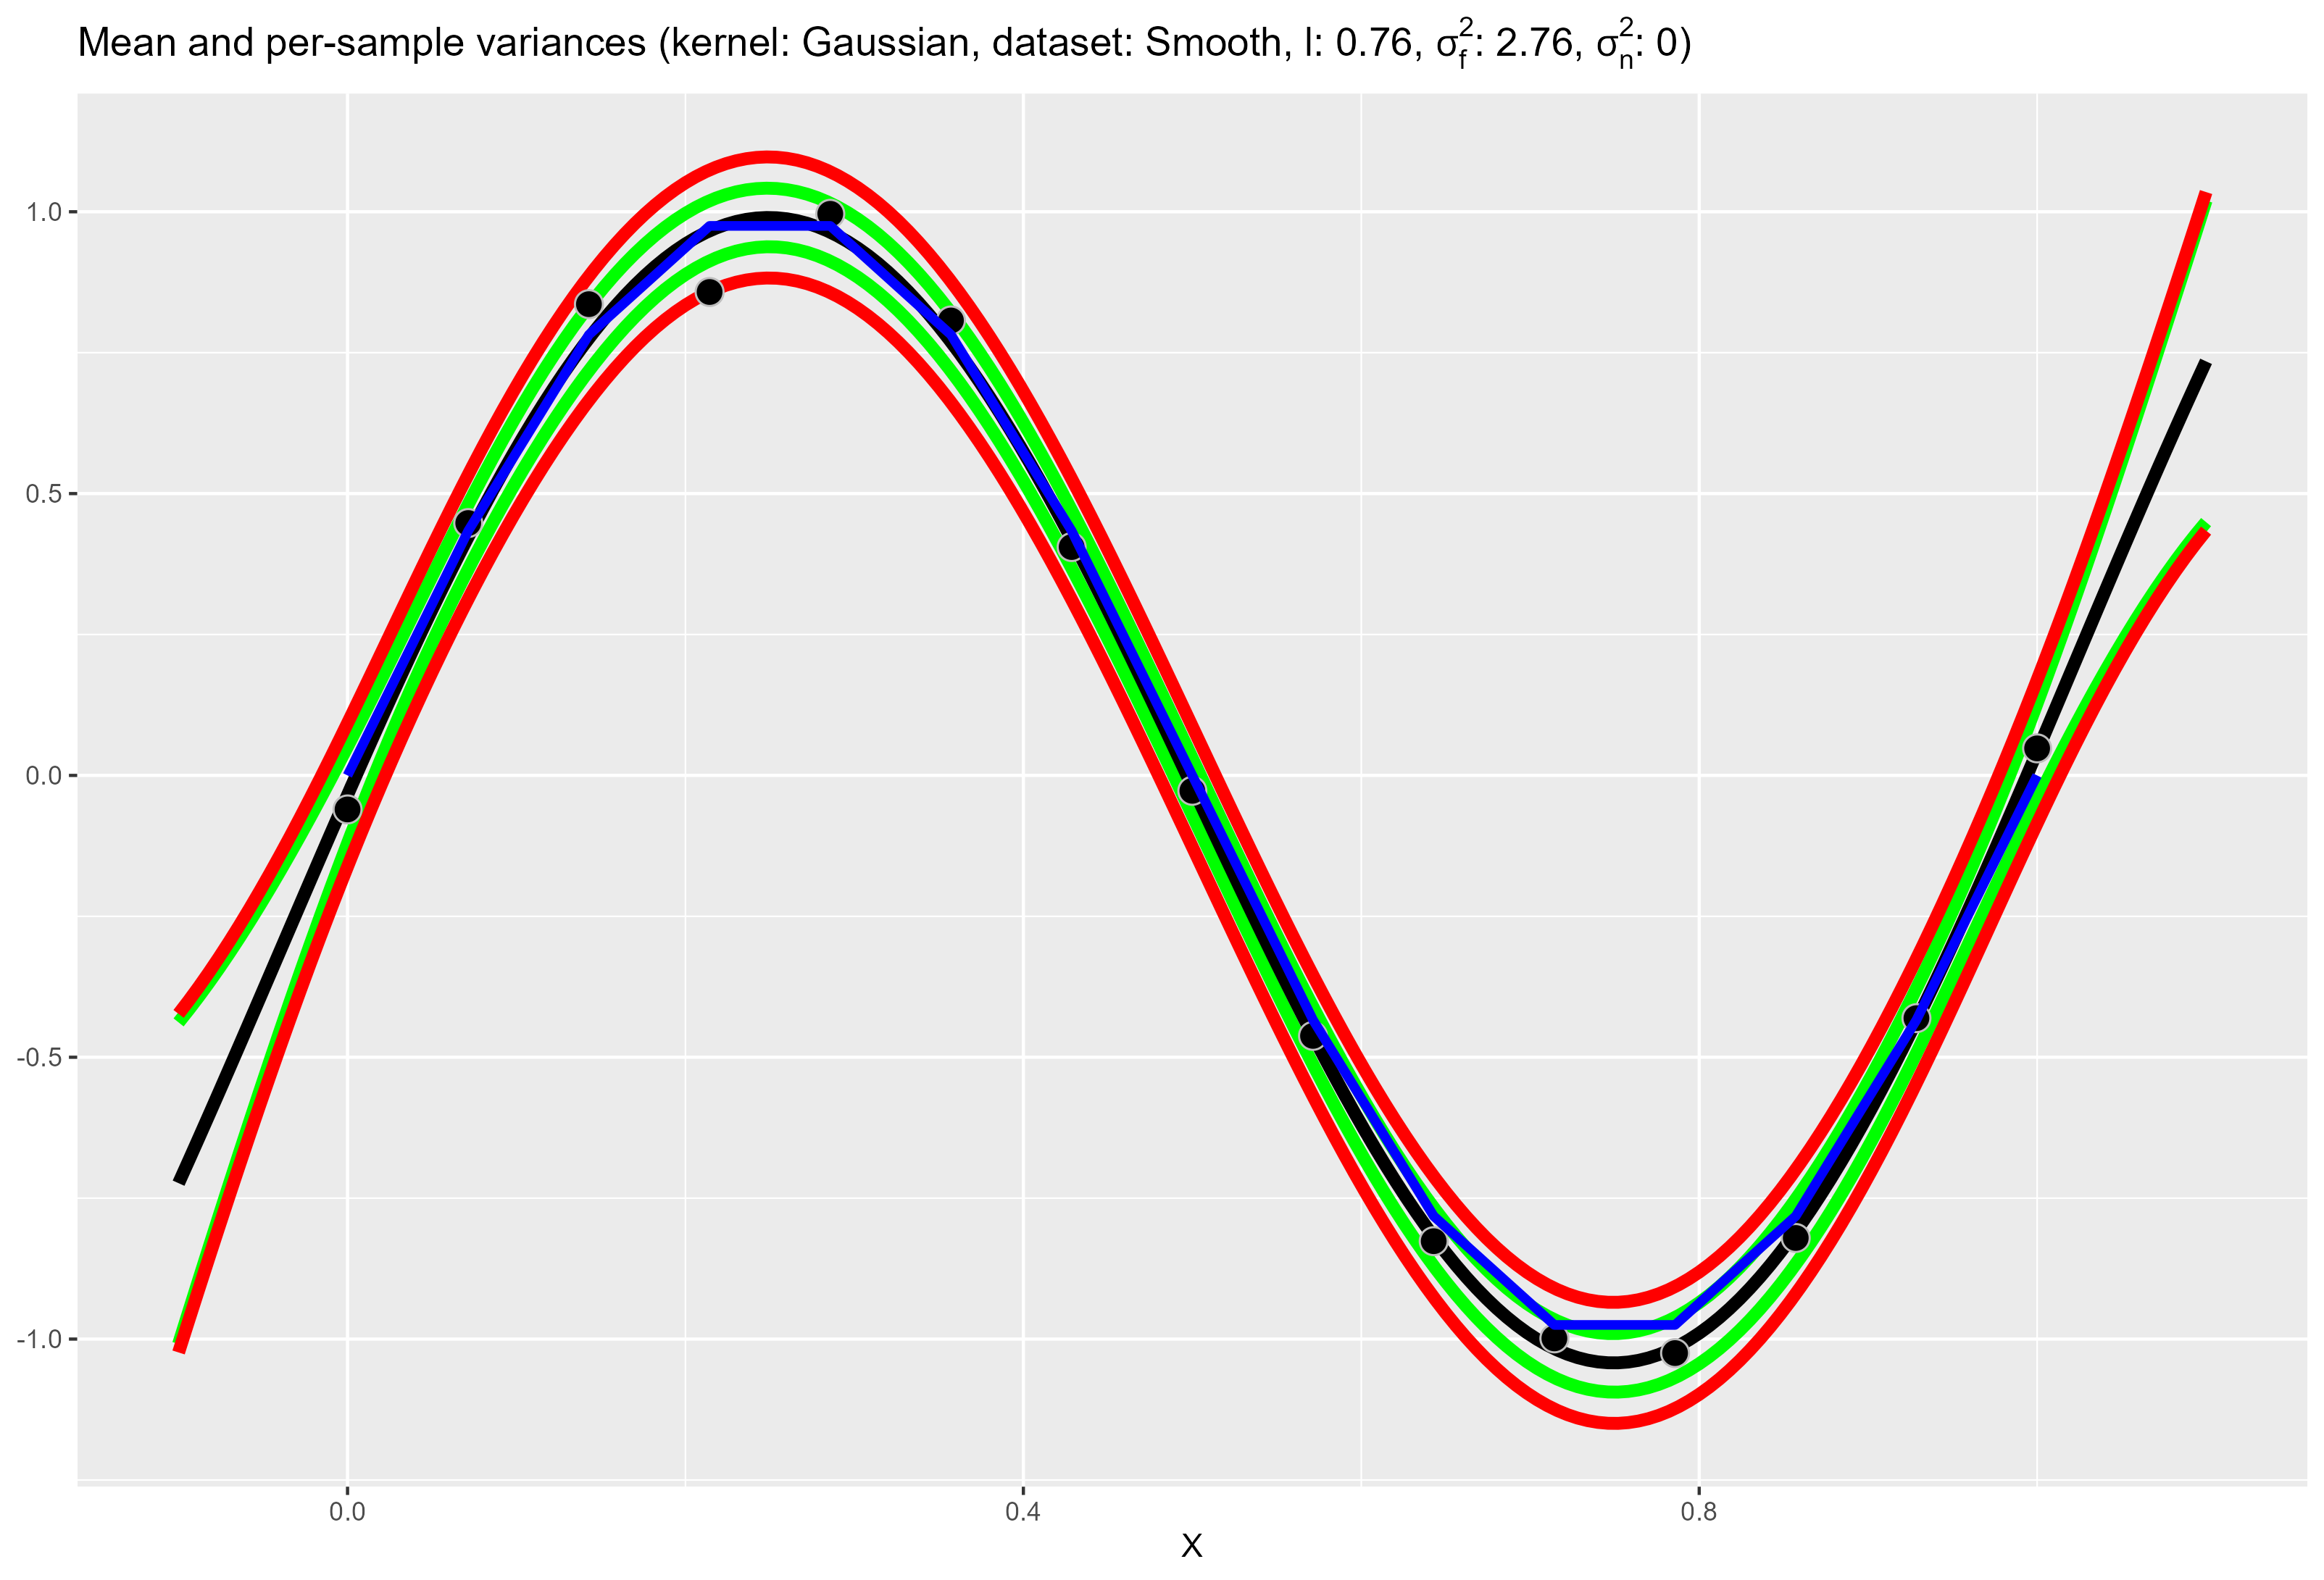
\includegraphics[height=0.5\textwidth]{covariance-functions/Gaussian_Smooth_mean.png}
    \caption{
        Plot of a GP using SE applied to a smooth sin wave $y = \sin(2 * pi * x) + \epsilon$, $\epsilon \sim N(0, 0.05)$, fitted using the R package GauPro \cite{gaupro}. \\
        The noiseless sin-wave is in blue and some sample datapoints taken from this function with noise are in black. The black line represents the expected function from the Gaussian process. The green line represents the 95\% confidence interval around the predictive distribution without the $\sigma^2_n$ term, representing the uncertainty surrounding predictions of the noise-free mean function $f(X)$. The red line represents the 95\% confidence interval with $\sigma^2_n$, representing the uncertainty surrounding predictions of the noisy observations $y$.
    }
\end{figure}
For this extremely smooth function with low noise, SE nearly perfectly captures the original data-generating function. The variances fall as they approach datapoints and rise as they move away from them. Defining our point of interest as $x_*$, as $x_*$ approaches a training datapoint $x$, $x - x*$ approaches zero and the value of our SE kernel approaches one, and the predictive distribution at $x_*$ collapses close to our training data $N(Y \sigma_n^2I, \sigma_n^2I)$. This is known as the interpolation property \cite{gp-ml} and is valid for all stationary covariance functions we cover.

\begin{figure}[H]
    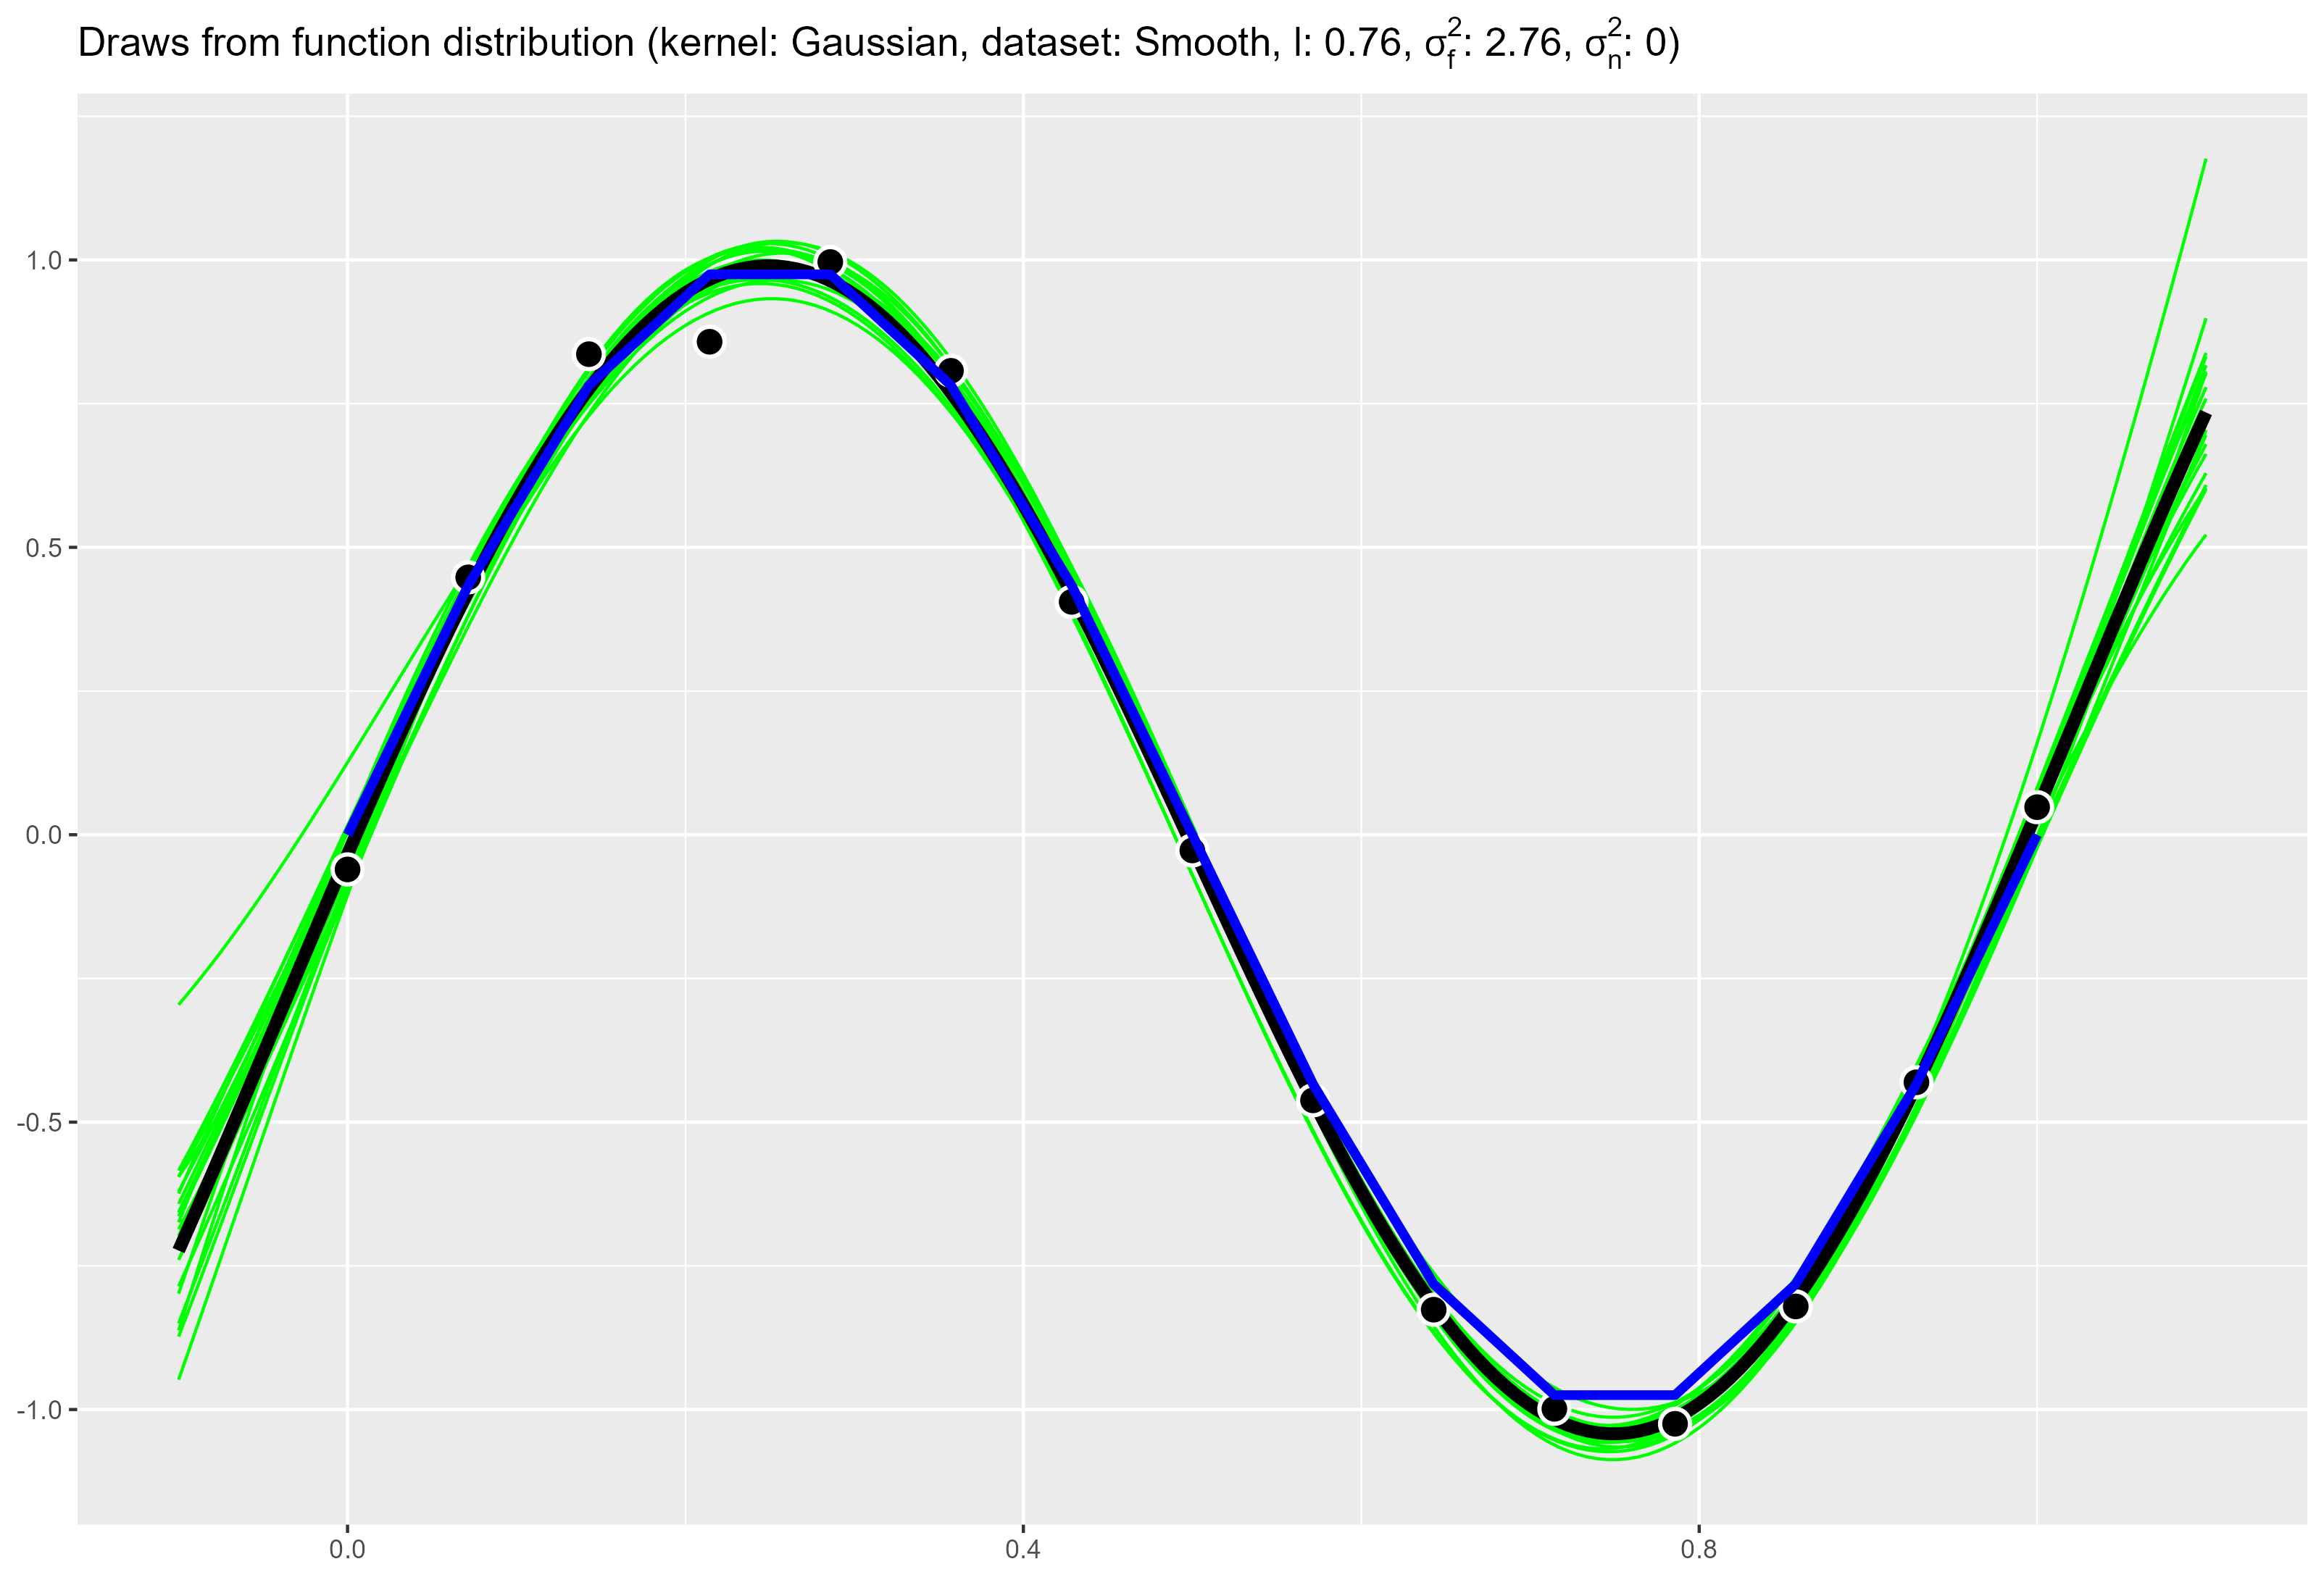
\includegraphics[height=0.5\textwidth]{covariance-functions/Gaussian_Smooth_draws.png}
    \caption{
        Plots of some sample functions drawn from a GP trained on the smooth dataset using SE. The blue and black lines are, as before, the noiseless data-generating function and the mean function drawn from the GP respectively. The green lines are 20 functions drawn from the GP - if we superimposed these draws onto the previous GP of means and variances, we would expect approximately 95\% of these function draws to be contained within the red variance lines. \\
            }
\end{figure}
Although we can technically draw infinite sample functions from any GP, these function draws all look very similar. This is because very few functions exist that satisfy SE's infinite smoothness and can exist entirely within this variance envelope, and they inevitably share many properties.

These constraints also affect the sample functions' ability to obey the interpolation property and require a trade-off between smoothness and fidelity. For example, there are no sample functions that pass through the fourth point at $(0.21, 0.86)$ because infinitely smooth functions are too rigid to pass through this point and the next two points at $(0.29, 1)$ and $(0.36, 0.81)$. This violation of the interpolation property is a consequence of the noise term $\epsilon \sim N(0, 0.05)$ in the data-generating function. If the noise term was zero and the data-generating function was infinitely differentiable, like this one, then the GP and all sample paths would pass through all datapoints.

\begin{figure}[H]
    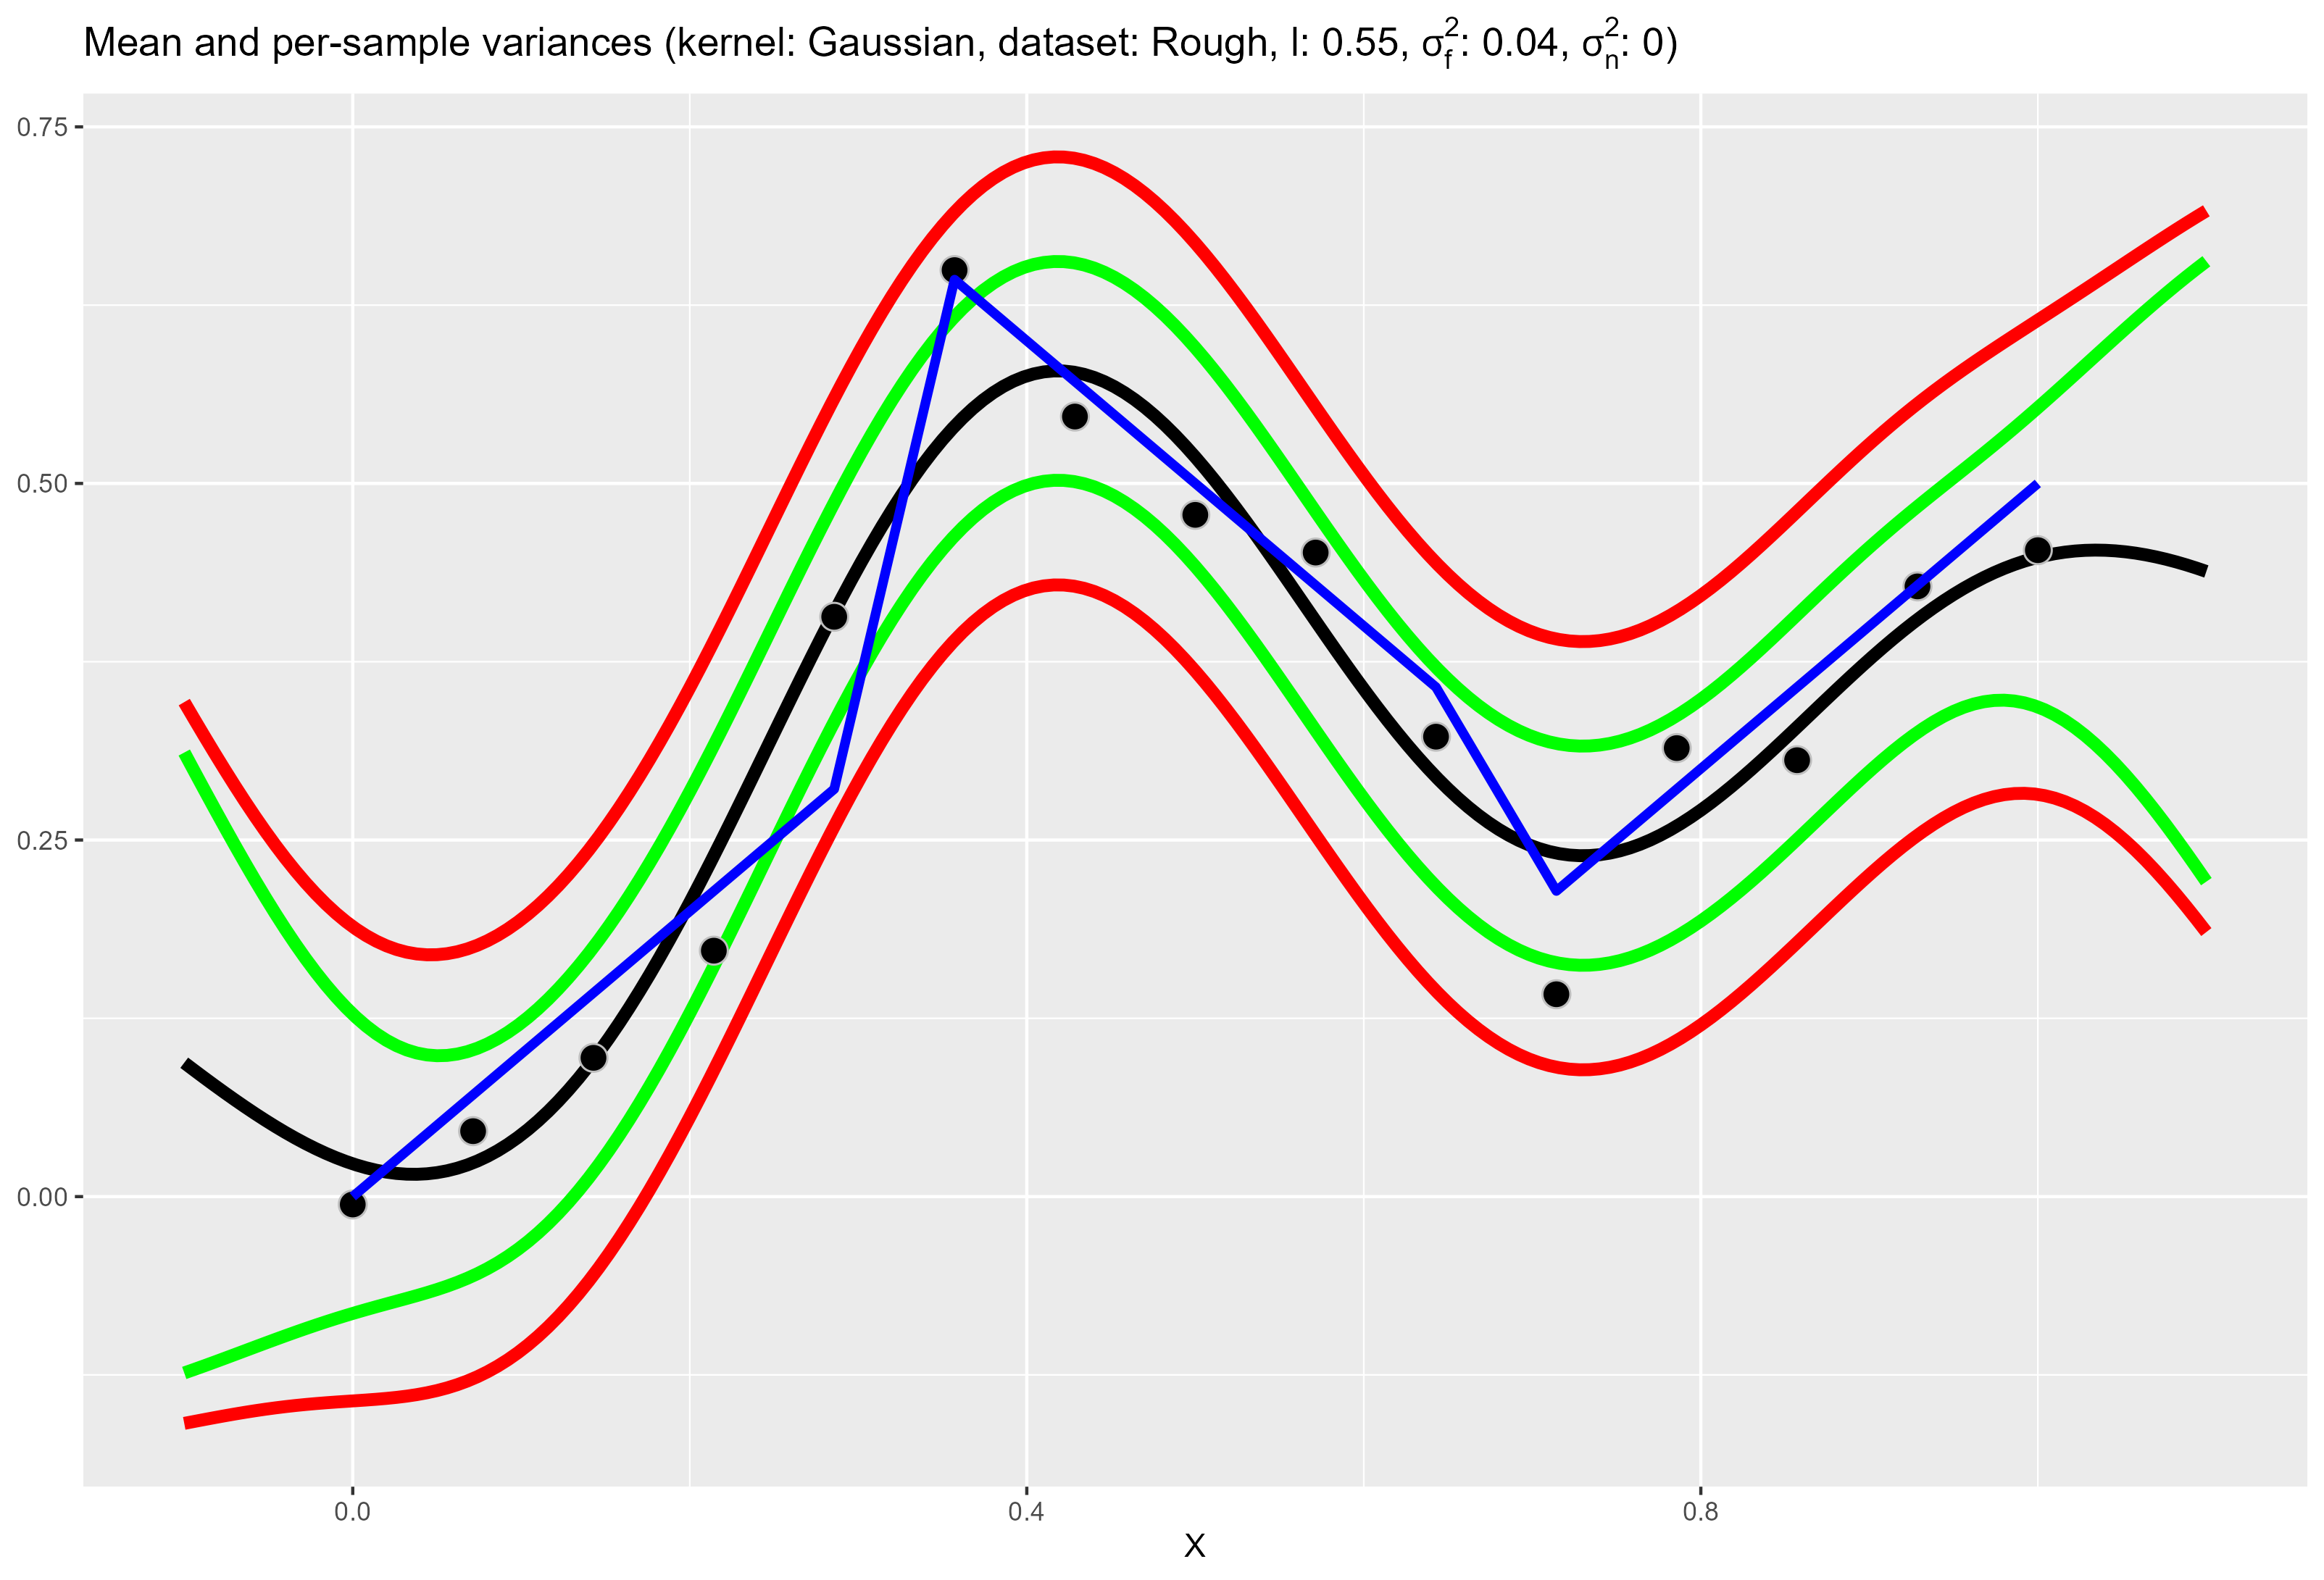
\includegraphics[height=0.5\textwidth]{covariance-functions/Gaussian_Rough_mean.png}
    \caption{Plot of the expected function draw and variances as before, using SE fitted to a rougher function:
        $\begin{cases}
                x < 0.3 & x \\
                0.3 \leq x < 0.7 & 1 - x \\
                x \geq 0.7 & x - 0.5
        \end{cases}$
    }
\end{figure}
SE performed worse on this rougher data as its extreme smoothness is unable to adapt well. The length scale has decreased (0.55, compared to 0.76 using smooth data), which reduces the rate of variance decay with frequency \ref{eq:se-sd} and increases the oscillatory behaviour of the GP sample functions whilst still producing infinitely smooth functions.

\begin{figure}[H]
    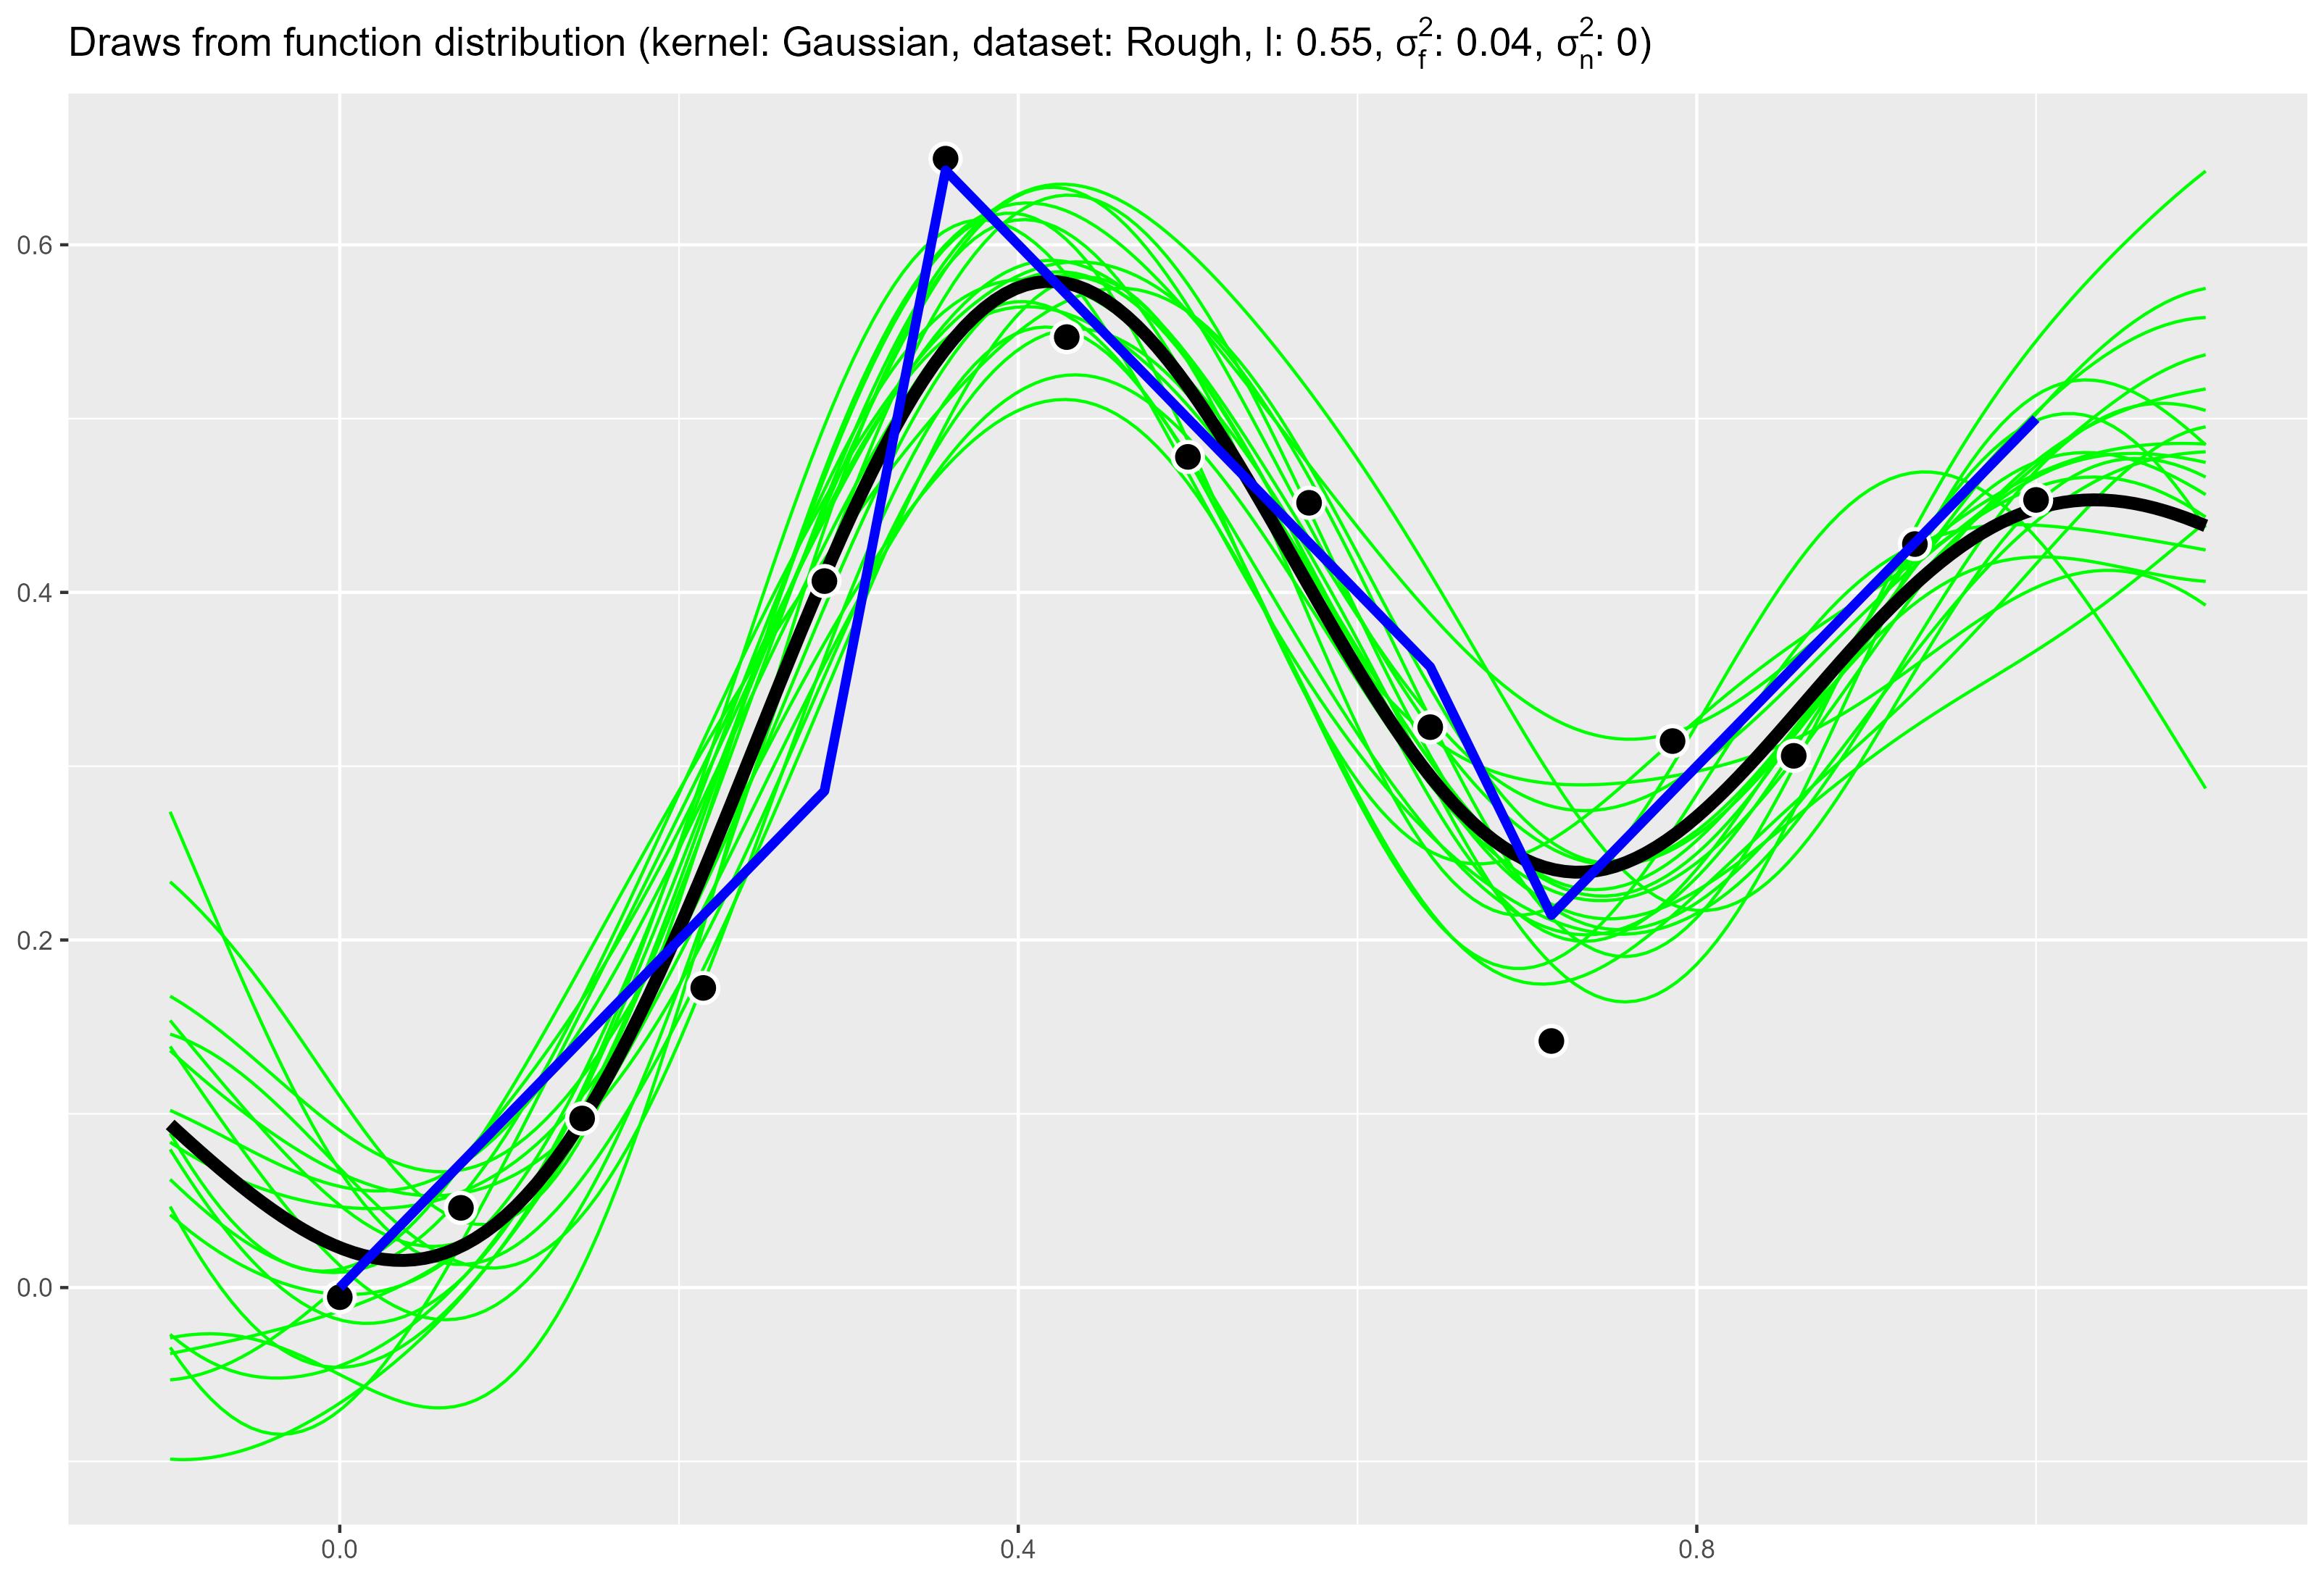
\includegraphics[height=0.5\textwidth]{covariance-functions/Gaussian_Rough_draws.png}
    \caption{Plot of some sample functions drawn from a GP as before, trained on the rough dataset using SE.
    }
\end{figure}
These functions are much more varied than those drawn from the smooth dataset, as SE is unable to adapt to the rougher data. Some draws have become more oscillatory due to the decrease in length scale, but all draws are still infinitely smooth.

\subsubsection{Rational quadratic (RQ)}
RQ controls smoothness by using a mixture of different length scales to capture multiple trends in the data at different frequencies. 
\begin{equation*}
    k(X,X') = \left( 1 + \frac{|X - X'|^2}{2\alpha l^2} \right)^{-\alpha}
\end{equation*}
We can derive this form by creating an infinite sum of different instances of SE with a vector of different length-scales $l$ and some weights $w_i$ attached to each instance:
\begin{equation*}
    k(X,X') = \sum_{i=1}^{\infty} w_i \exp \left( -\frac{|X - X'|^2}{2l_i^2} \right)
\end{equation*}
This is a valid covariance function long as the sum remains less than $\infty$ to maintain PSD. We can turn this into a continuous representation if our $l$ is very dense, where $p(l)$ is the PDF for $l$:
\begin{equation*}
    k(X,X') = \int_{0}^{\infty} p(l) \exp \left( -\frac{|X - X'|^2}{2l^2} \right) dl
\end{equation*}
Defining $\tau= l^{-2}$, $l = \tau^{-1/2}$. Putting this into SE:
\begin{equation*}
    k_{SE}(X,X') = \exp(-\frac{|X - X'|^2}{2[\tau^{-1}]}) = \exp(-\frac{1}{2} \tau |X - X'|^2)
\end{equation*}
Before putting this back into the above integral which is in terms of $l$, we need to account for the change of variables from $l$ to $\tau$. The Jacobian factor of this transformation is:
\begin{equation*}
    | \partial_{\tau} l | = \frac{1}{2} \tau^{-3/2} d\tau
\end{equation*}
Defining the transformation $l(x) = \frac{1}{\sqrt{x}}$, putting these into the integral changes the PDF from $p(l)$ to $p(l(\tau)) | \partial_{\tau}l |$:
\begin{equation*}
    k(X,X') = \int_{0}^{\infty} p(l(\tau)) \frac{1}{2} \tau^{-3/2} \exp \left( -\frac{1}{2} \tau |X - X'|^2 \right) d\tau
\end{equation*}
We need an expression for the PDF $p(\tau)$ that integrates to $1$ and is PSD. A common choice is the Gamma distribution with shape $\alpha$ and scale $\beta$ parameters: $\tau \sim \Gamma(\alpha, \frac{\beta}{\alpha})$ 
\begin{equation*}
    p(\tau) \propto \tau ^{\alpha - 1} \exp \left( - \frac{\alpha}{\beta} \tau \right)
\end{equation*}
Putting this into the integral:
\begin{equation*}
    k(X,X') \propto \int_{0}^{\infty}  \left[ \tau^{\alpha - 1} \exp \left(-\frac{\alpha}{\beta} \tau \right) \right] \frac{1}{2}\tau^{-3/2} \exp \left( \tau - \frac{1}{2} \tau |X - X'|^2 \right) d\tau
\end{equation*}
$\frac{1}{2}\tau^{-3/2}$ from $dl$ and the new $\tau^{a-1}$ combine, and the new exponential joins the existing one:
\begin{equation*}
    k(X,X') \propto \int_{0}^{\infty} \frac{1}{2} \tau^{\alpha - \frac{5}{2}} \exp \left[ -\tau \left( -\tau\frac{\alpha}{\beta} + \tau \frac{|X - X'|^2}{2} \right) \right] d\tau
\end{equation*}
We can use the Gamma integral here, but need some rearranging. Absorbing $\frac{1}{2}$ into the proportionality, setting $a = \alpha - \frac{3}{2}$ and factoring $\tau$ out of the exponent for $c = \frac{\alpha}{\beta}\tau + \frac{|X - X'|^2}{2}$:
\begin{equation*}
    k(X,X') \propto \int_{0}^{\infty} \tau^{a - 1} \exp ( -\tau c ) d\tau
\end{equation*}
Applying the Gamma integral and absorbing $\Gamma(a)$ into proportionality:
\begin{equation*}
    k(X,X') \propto c^{-a} \Gamma(a) \propto \left[ \frac{\alpha}{\beta} + \frac{|X - X'|^2}{2} \right]^{-\left( \left[ \alpha - \frac{3}{2} \right] \right)} 
\end{equation*}
Now we need to decide on the parameter values of our Gamma distribution. Since the Gamma distribution strictly takes in one Typically, $\beta = l^-2$ such that $\beta^{-1} = l^2$ and $\frac{\alpha}{\beta} = a \cdot \beta^{-1} = \alpha l^2$. Substituting:
\begin{equation*}
    k(X,X') = \left( al^2 + \frac{|X - X'|^2}{2} \right)^{-\alpha - \frac{3}{2}}
\end{equation*}
Factoring out $al^2$ and absorbing it into the proportionality constant to get our final form:
\begin{equation*}
    k(X,X') = \left( 1 + \frac{|X - X'|^2}{2\alpha l^2} \right)^{-\alpha - \frac{3}{2}}
\end{equation*}
This derivation starts from the discrete length scale $l$ for illustrative purposes, so includes $\frac{3}{2}$ to account for the change from length scale to $\tau$. In practice, derivations start from $\tau$ so never have to change units and never include the $\frac{3}{2}$ term in the exponent.

RQ is infinitely MS differentiable, so produces infinitely smooth functions no matter what the shape parameter of our distribution of length scales $\alpha$ is. As $\alpha \to \infty$, this distribution becomes sharply peaked at a single length scale $l$ and RQ becomes SE. However, as $\alpha \to 1$, we get a wider spread of length scales and our sample functions capture trends at different frequencies. 

\begin{figure}[H]
    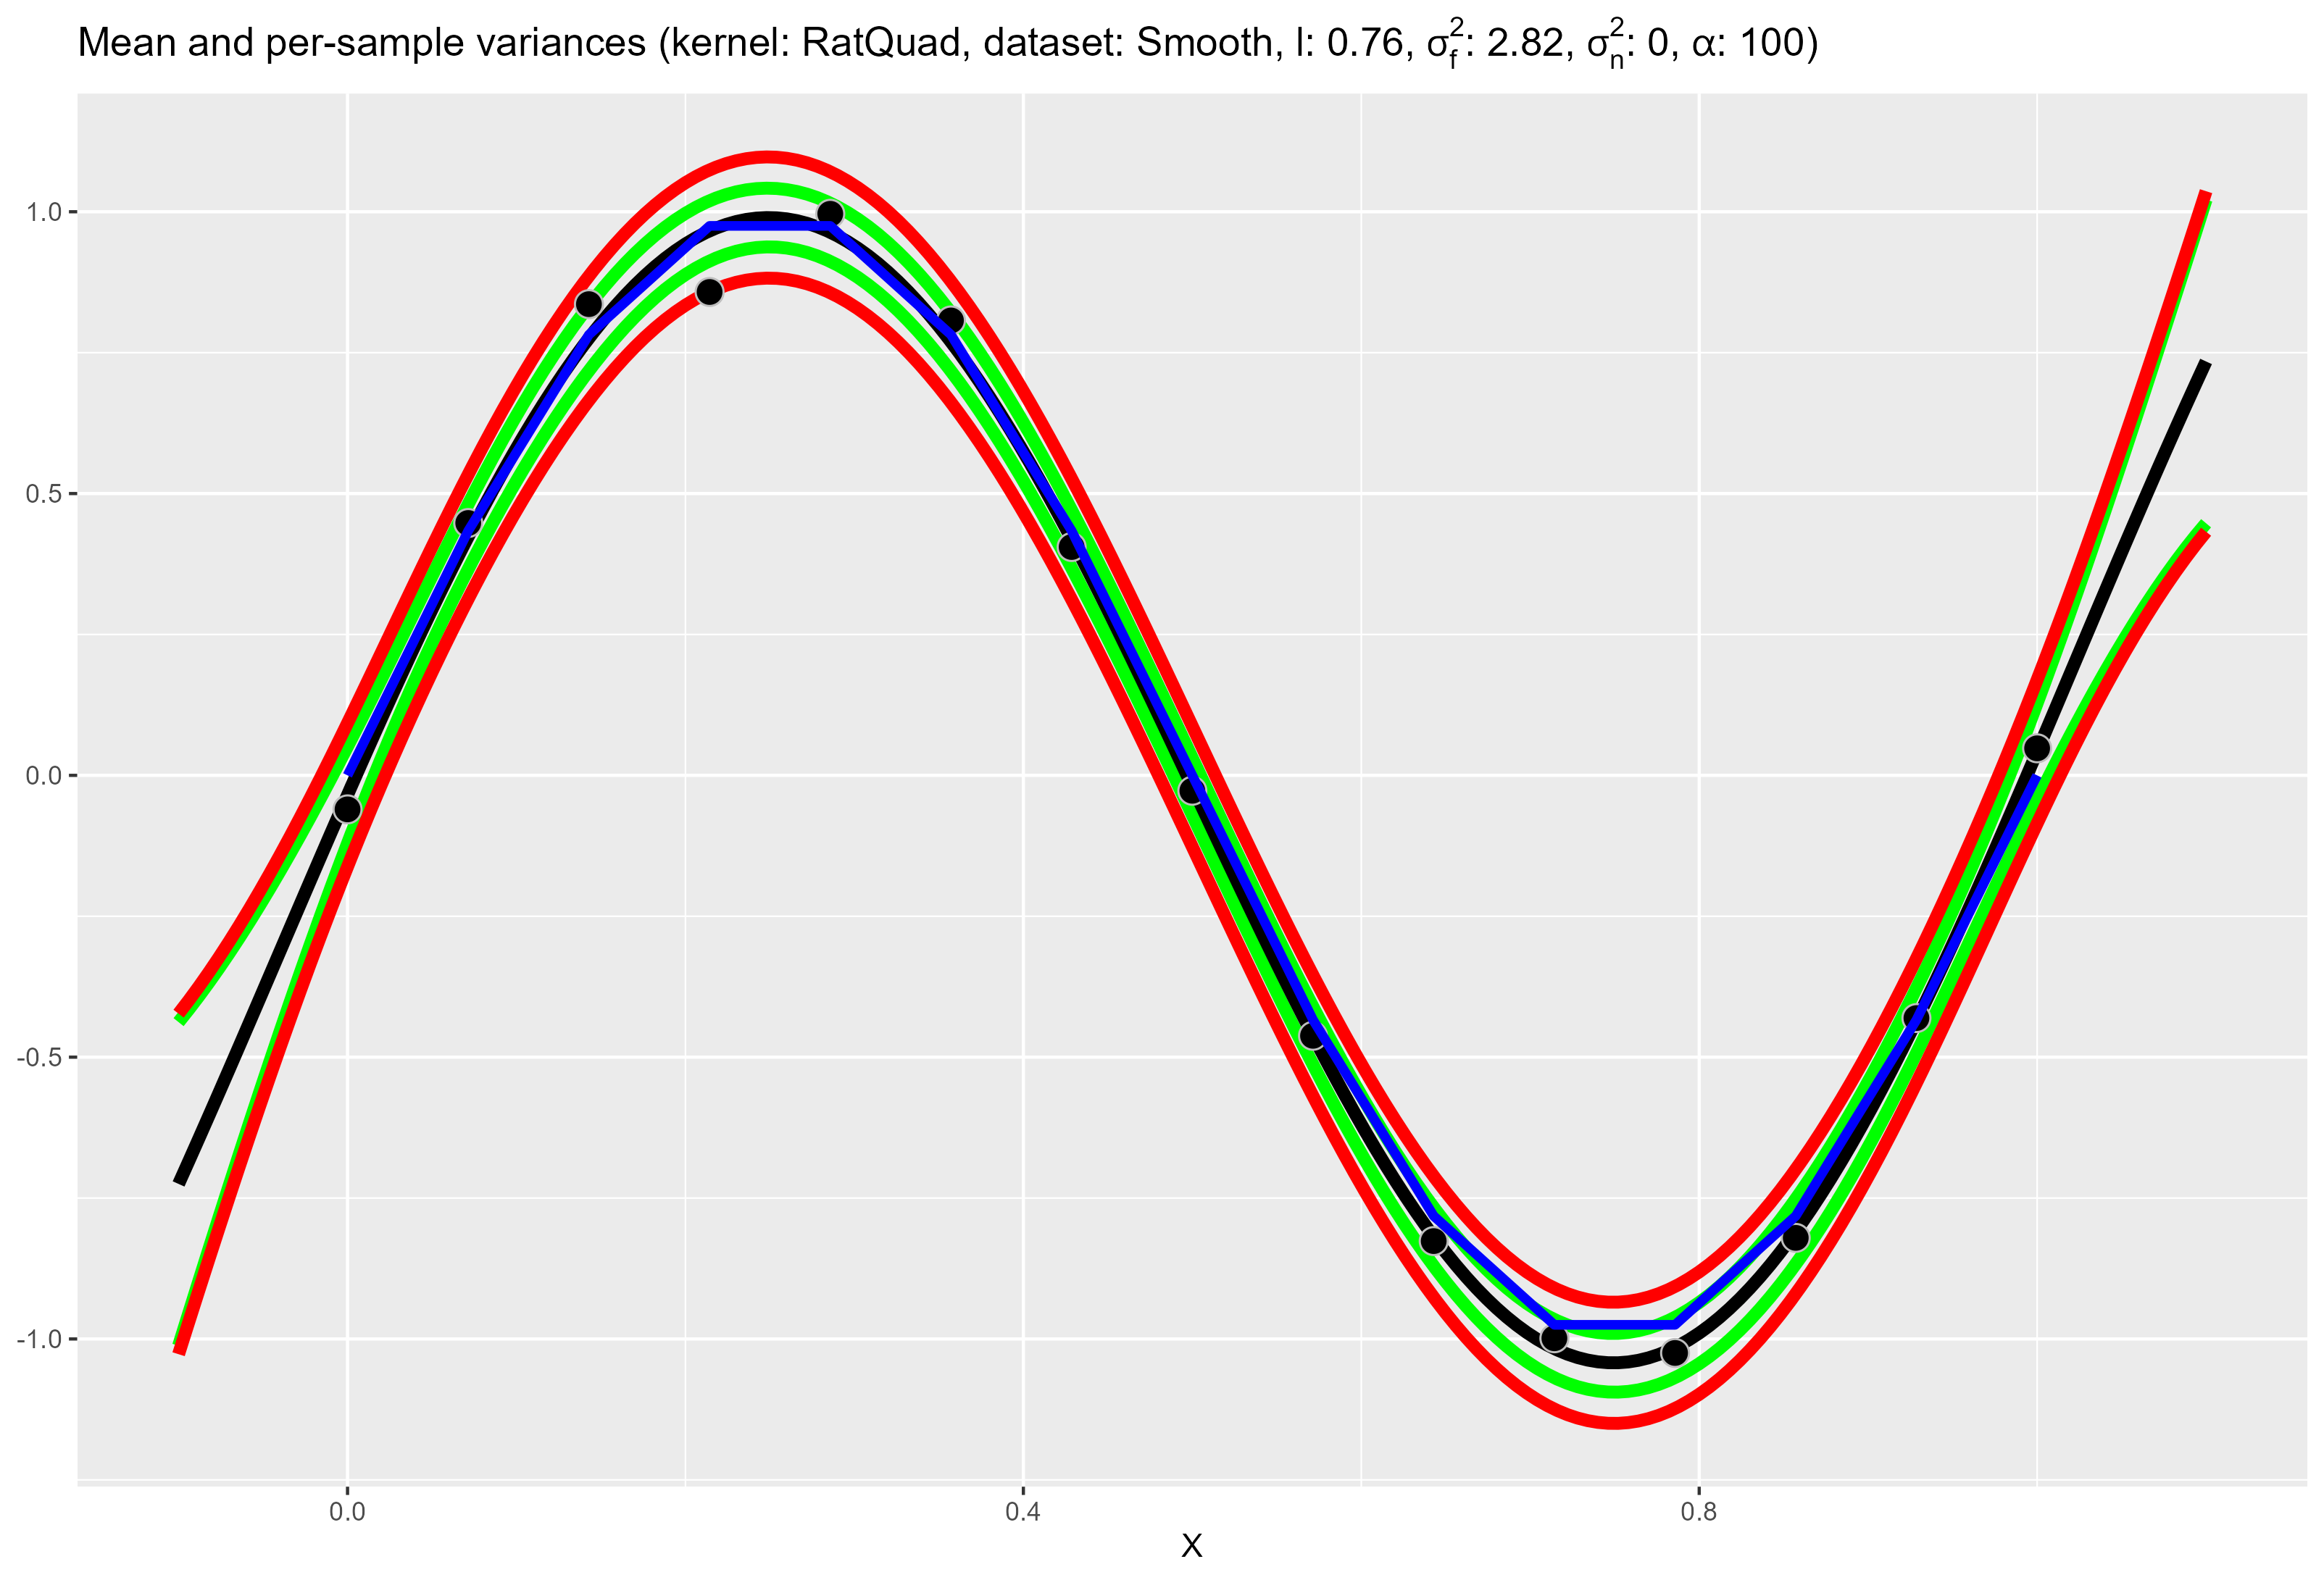
\includegraphics[height=0.5\textwidth]{covariance-functions/RatQuad_Smooth_mean.png}
    \caption{
        Plot of the expected function draw and variances as before, using RQ fitted to the smooth sin wave dataset.
    }
\end{figure}
The GauPro package \cite{gaupro} in R used to fit these GPs has chosen an extremely high $\alpha = 100$ via MLE because of the smoothness of the data-generating function. This high $\alpha$ means we are very likely to choose one length scale $l$ and thus RQ is nearly indistinguishable from SE.

\begin{figure}[H]
    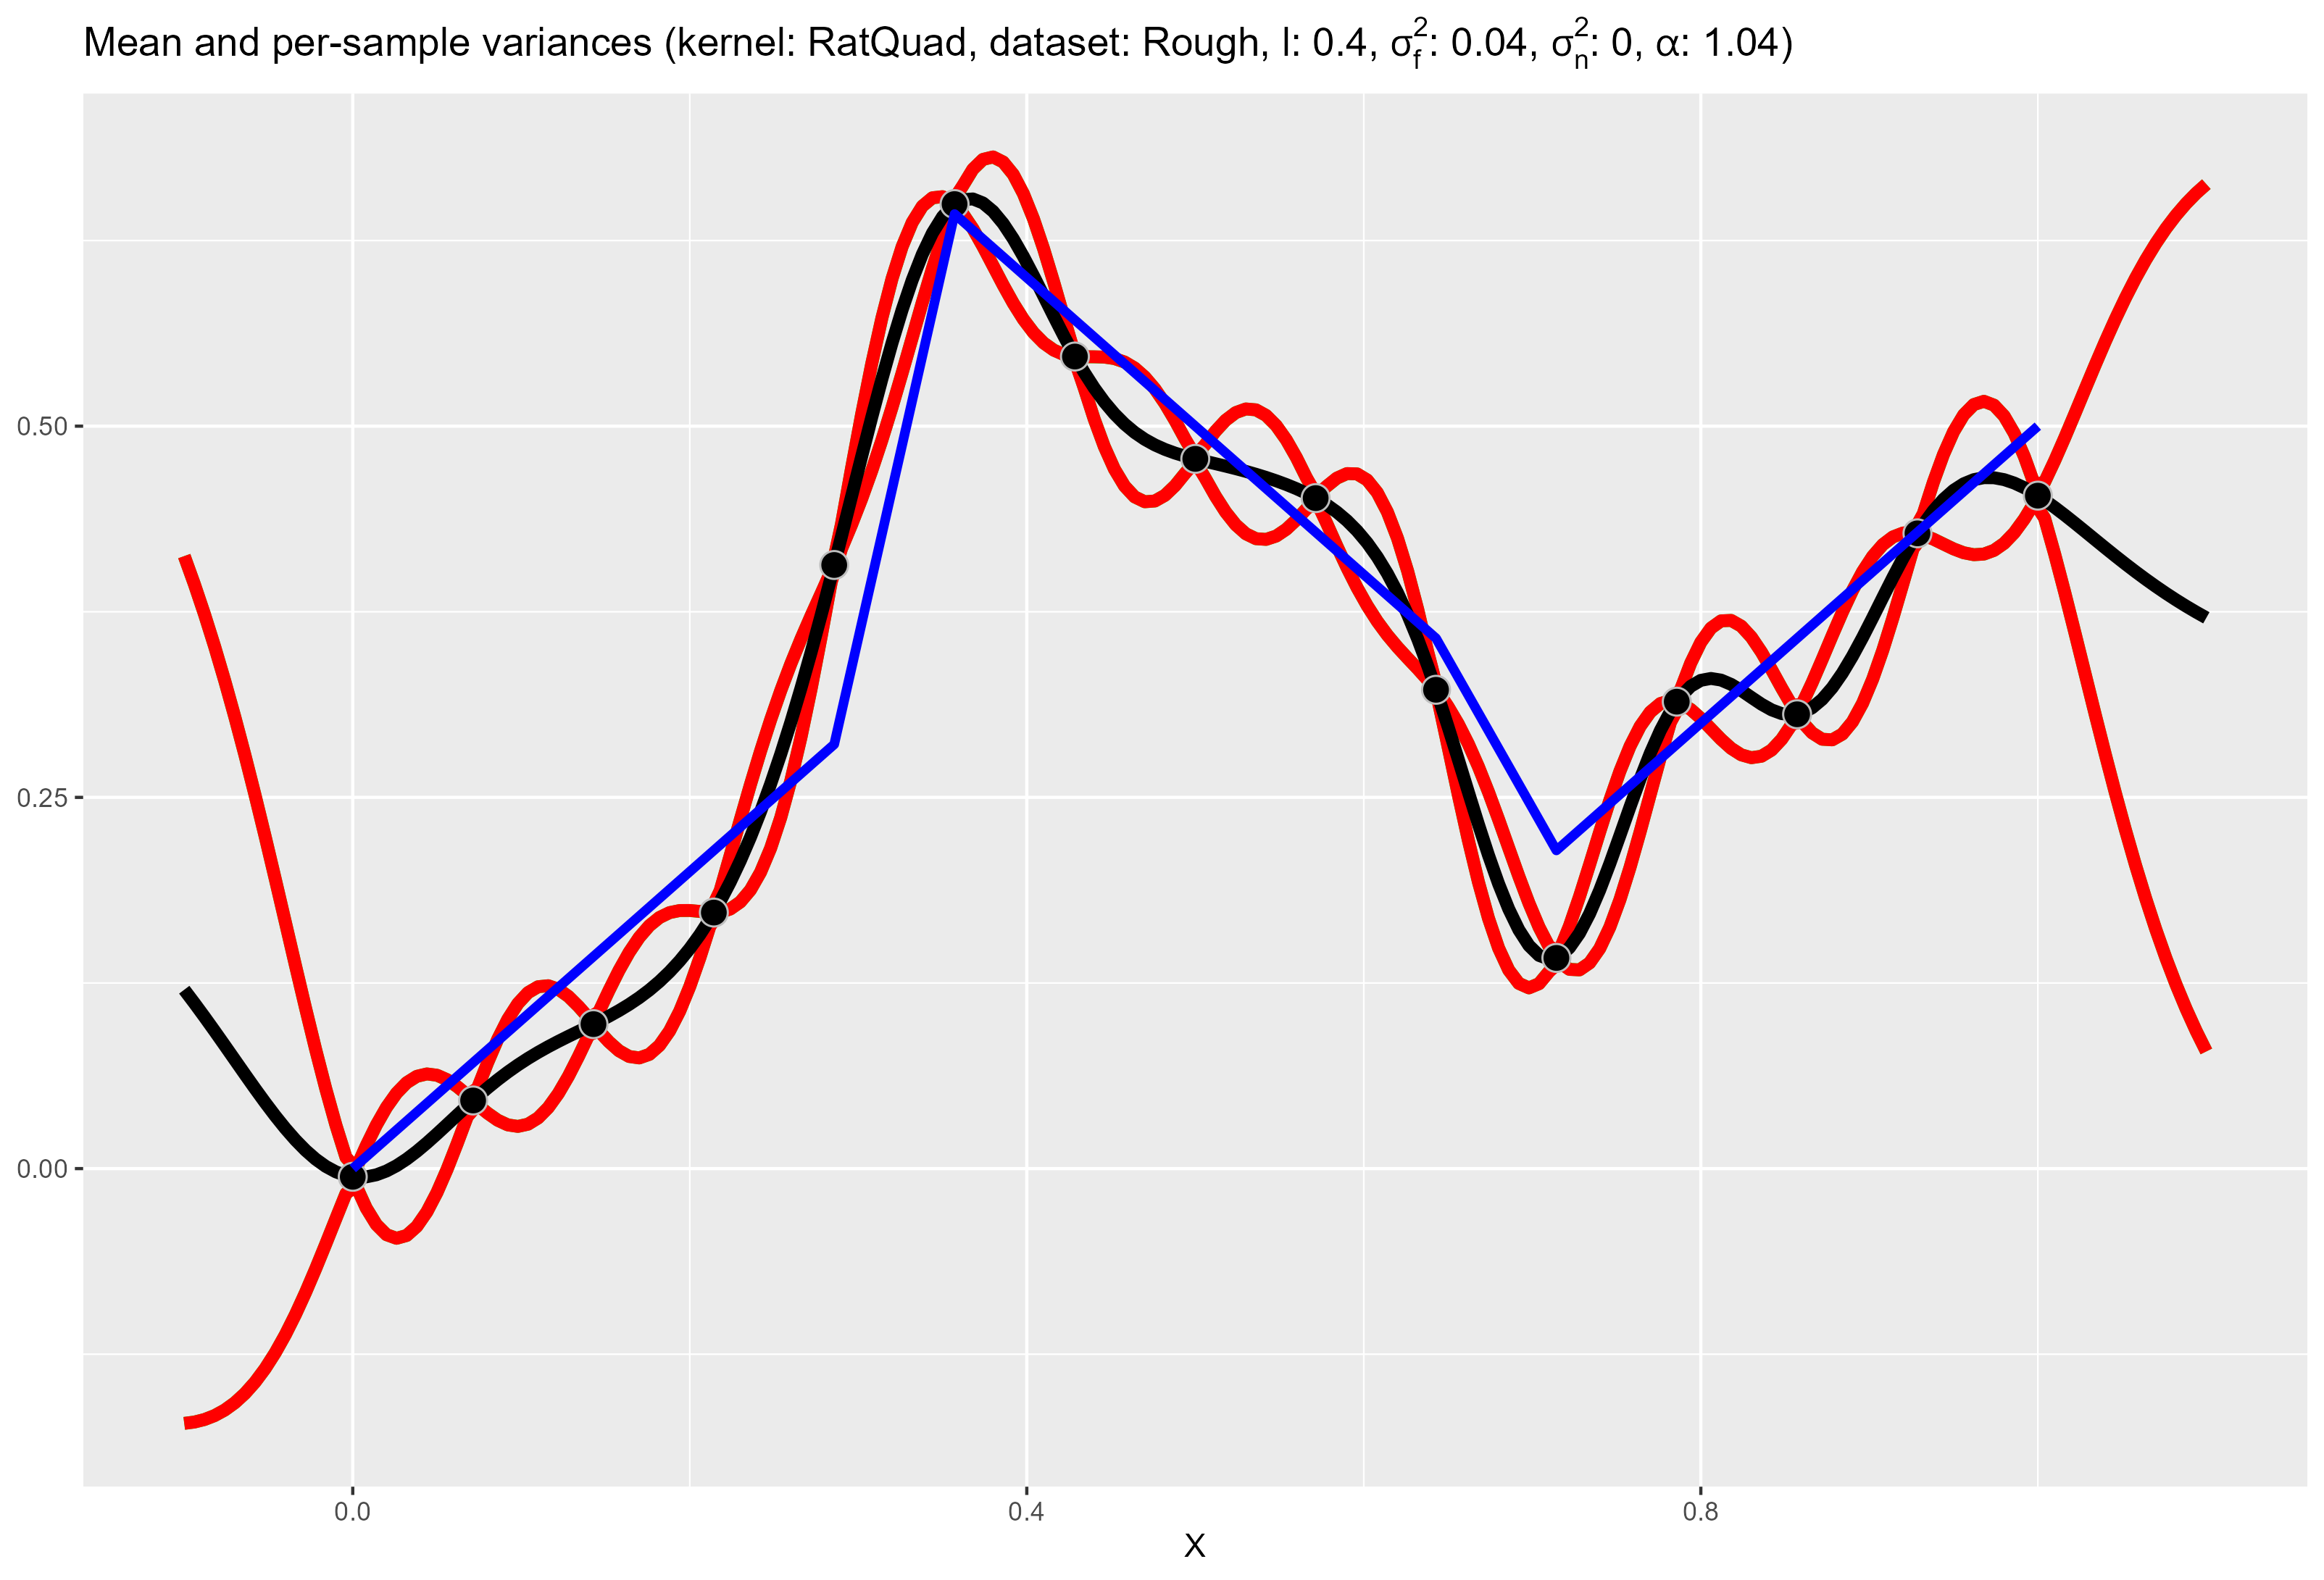
\includegraphics[height=0.5\textwidth]{covariance-functions/RatQuad_Rough_mean.png}
    \caption{
        Plot of the expected function draw and variances as before, using RQ fitted to the rougher dataset. \\
    }
\end{figure}
The rougher dataset has driven $\alpha$ to be much lower than in the smooth dataset, at $\alpha = 1.04$, and RQ becomes a true heavy-tailed mixture distribution of SEs over length scales.

The green variance lines disappear because the expected sample path passes through all datapoints, so any new training point is expected to be exactly equal to the expected function draw at that point, and the variance is zero. If the data-generating function became too rough or we used a more inflexible kernel like SE, we would need these sample variance lines to reflect how far from the expected function draw we expect the sample functions to be. 

\begin{figure}[H]
    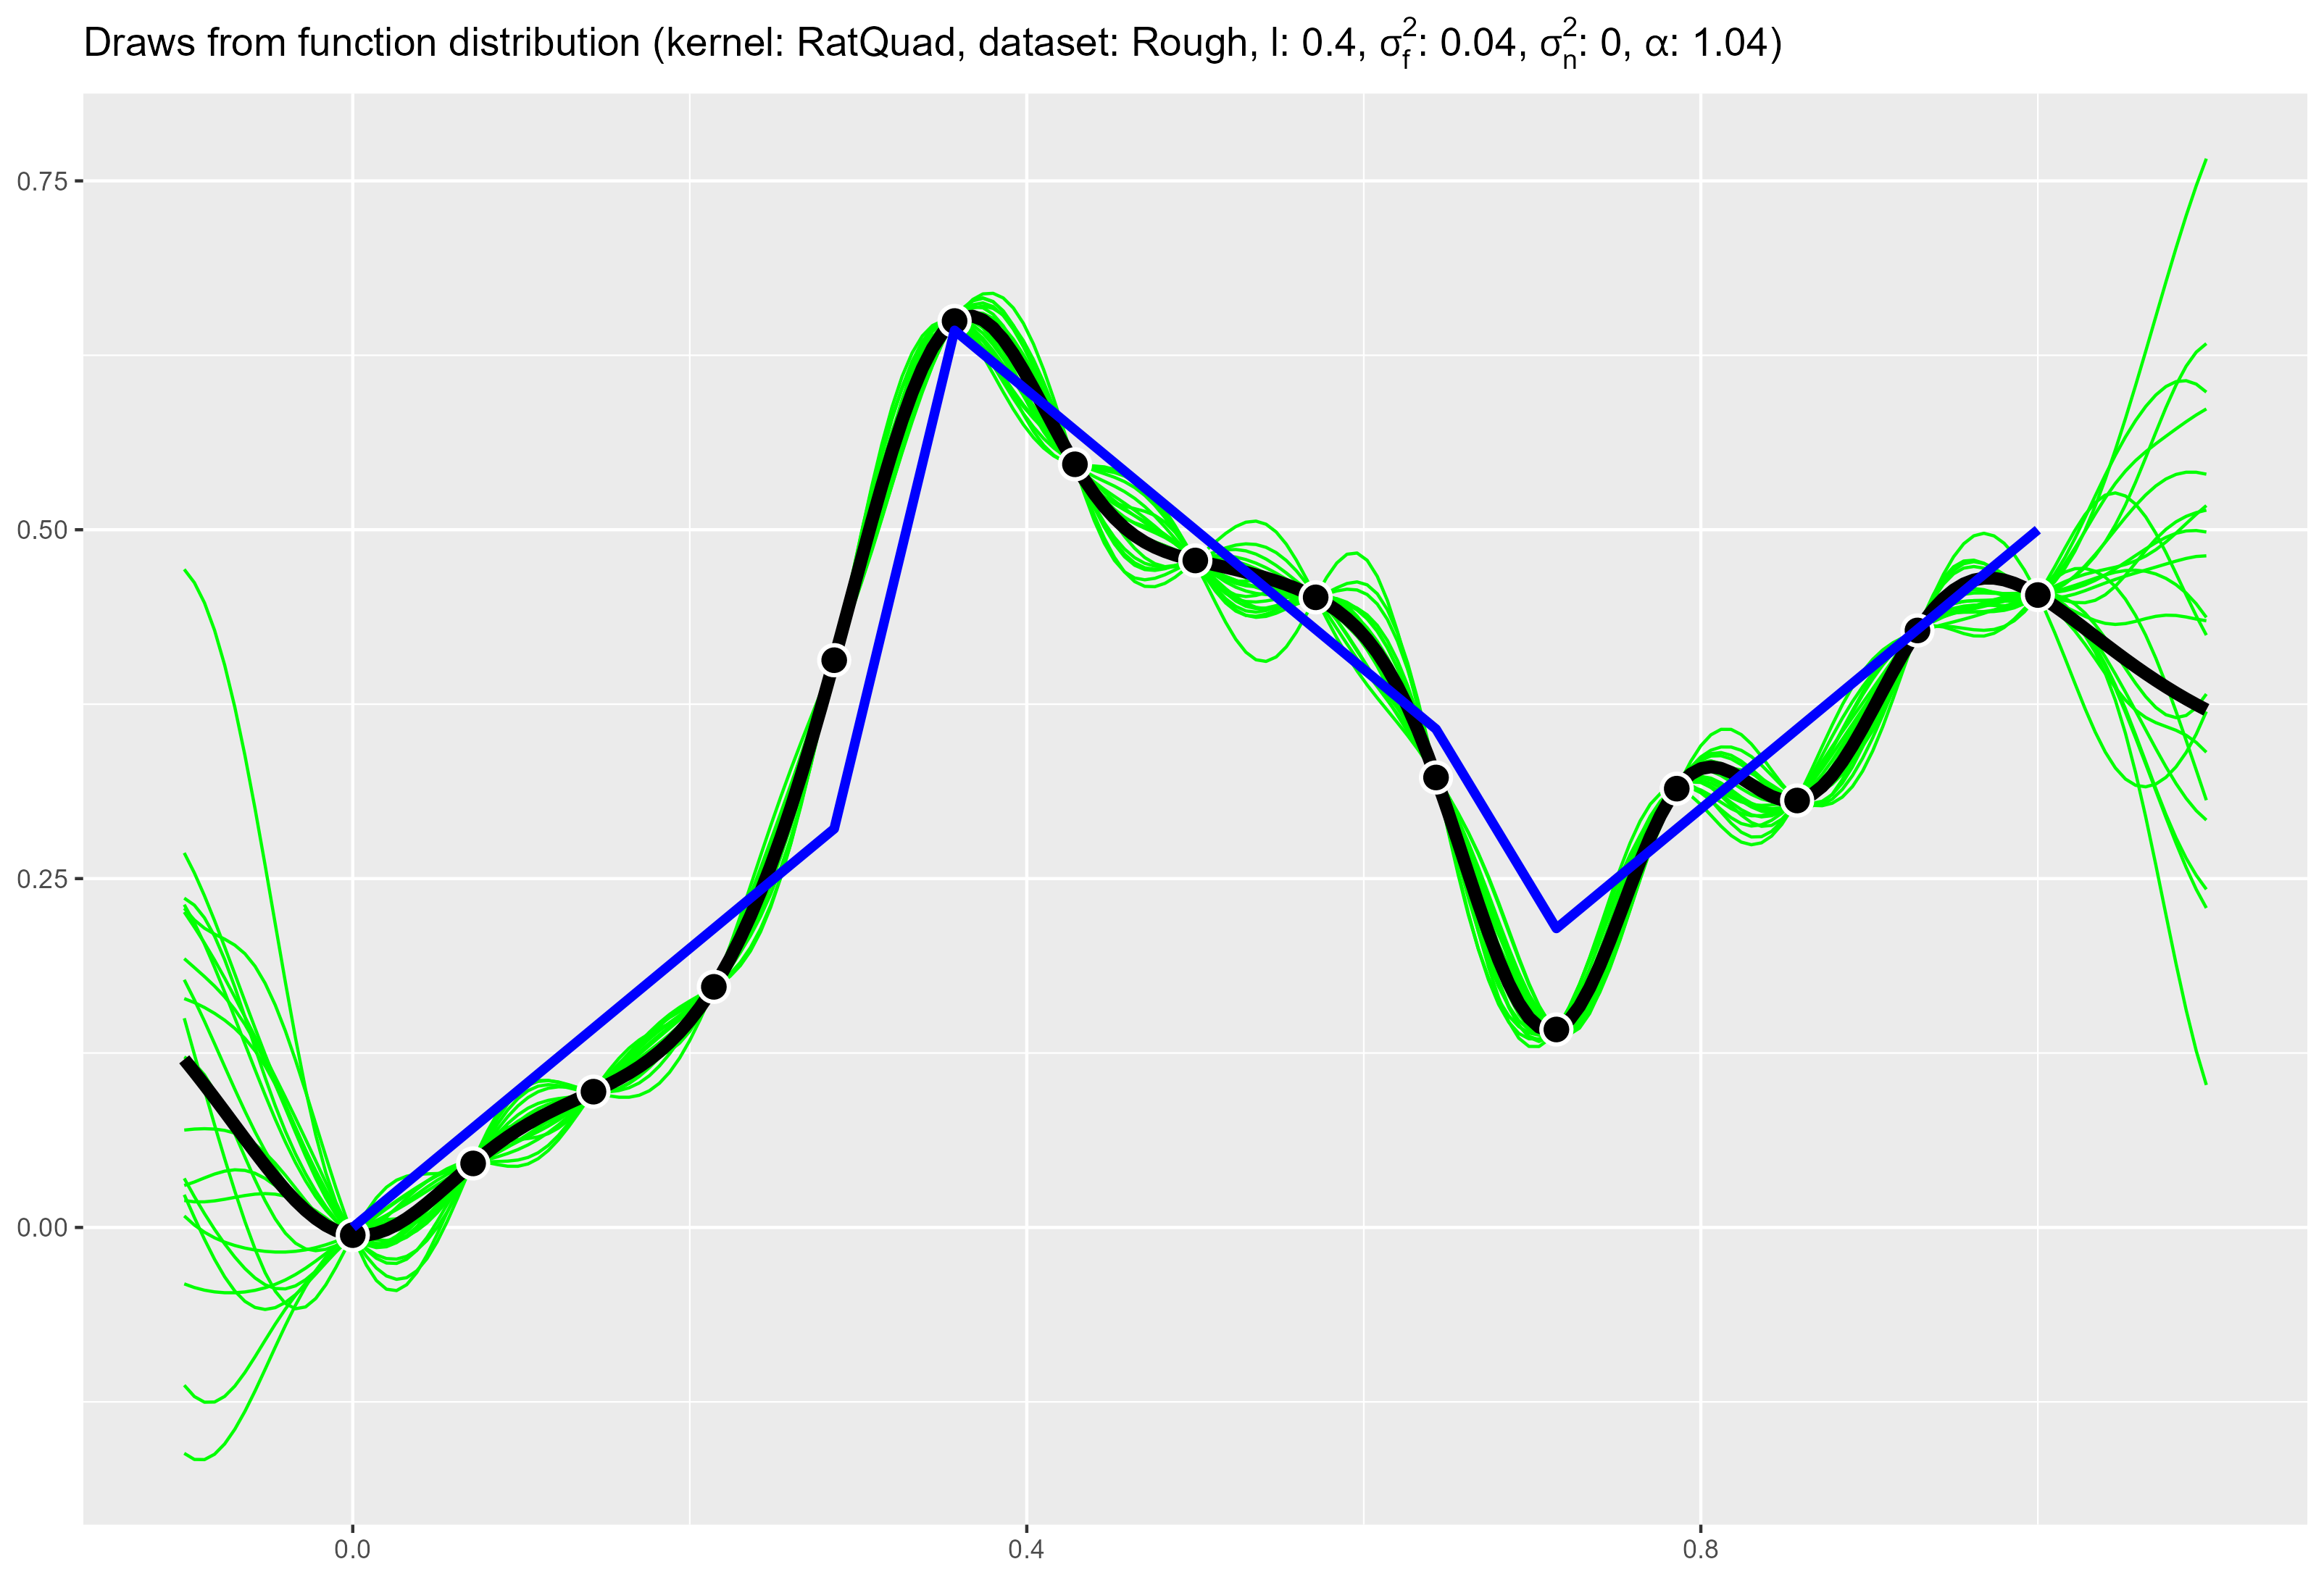
\includegraphics[height=0.5\textwidth]{covariance-functions/RatQuad_Rough_draws.png}
    \caption{
        Plots of some sample functions drawn from a GP as before, trained on the rough dataset using RQ.
    }
\end{figure}
Each function draw expresses a different combination of high and low length scale components drawn from this fixed inverse-gamma distribution, and exhibit different behaviours at different frequencies. This is especially visible as the difference between function draws widens between data points - some function draws oscillate less than others as they are capturing a longer-term, low-frequency trend in the data. These more flexible functions are enough for the expected function draw to pass through all datapoints and satisfy the interpolation property.

\subsubsection{$\gamma$-exponential and exponential}
RQ controlled smoothness by using a mixture of different length scales to capture multiple trends in the data at different frequencies. Another approach to controlling smoothness involves introducing a differentiability parameter $\gamma$ to control how differentiable the covariance function is and thus how smooth the sample functions are:
\begin{equation*}
    k(X,X') = \exp \left(-\frac{|X - X'|^{\gamma}}{l^{\gamma}} \right)
\end{equation*}
where $0 < \gamma \geq 2$ controls the smoothness of the covariance function. 
$\gamma = 2$ produces SE for maximal smoothness. For all other values of $\gamma$ other than $2$, the covariance function is continuous but not differentiable at all at $|x - x'| = 0$ because this point coincides with the undifferentiable turning point of the modulus function at $x - x' = 0$.

\begin{figure}[H]
    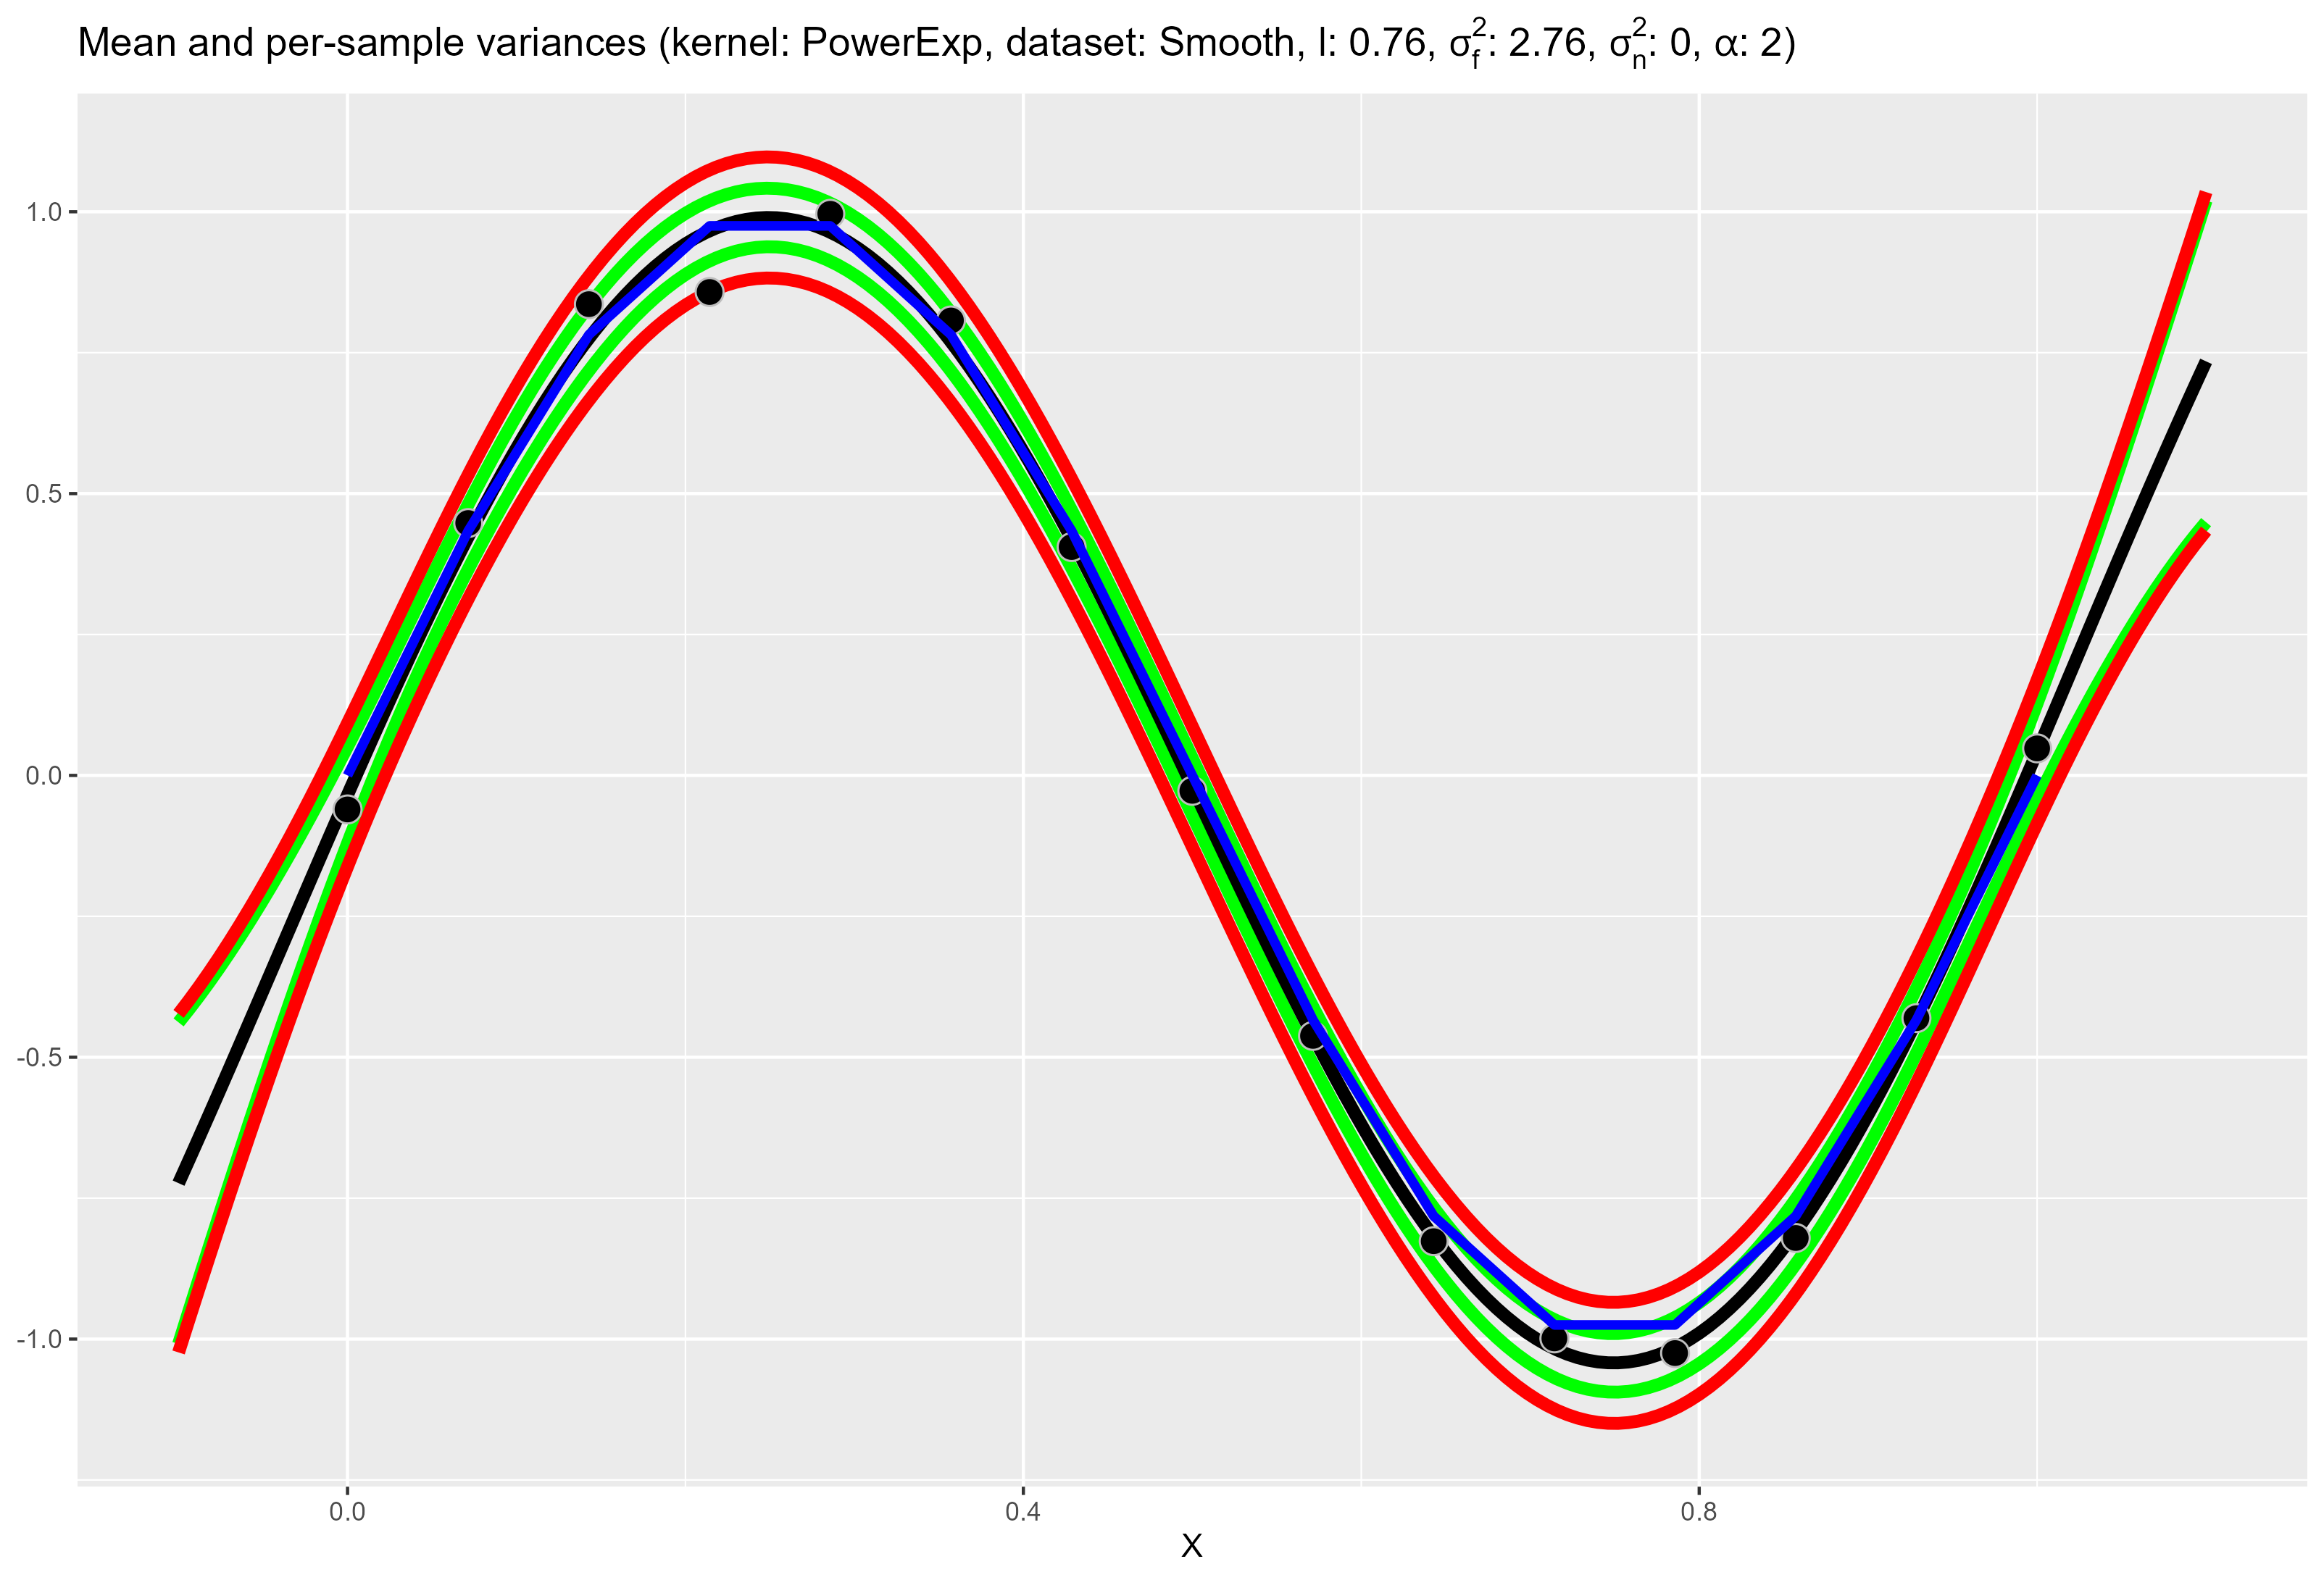
\includegraphics[height=0.5\textwidth]{covariance-functions/PowerExp_Smooth_mean.png}
    \caption{
        Plot of the expected function draw and variances as before, using $\gamma$-exponential fitted to the smooth sin wave dataset. \\ 
    }
\end{figure}
The GauPro package \cite{gaupro} in R has chosen $\gamma = 2$ via MLE, which produces SE. This is because the smoothness of the data-generating function is so high that no other covariance function can capture it.

\begin{figure}[H]
    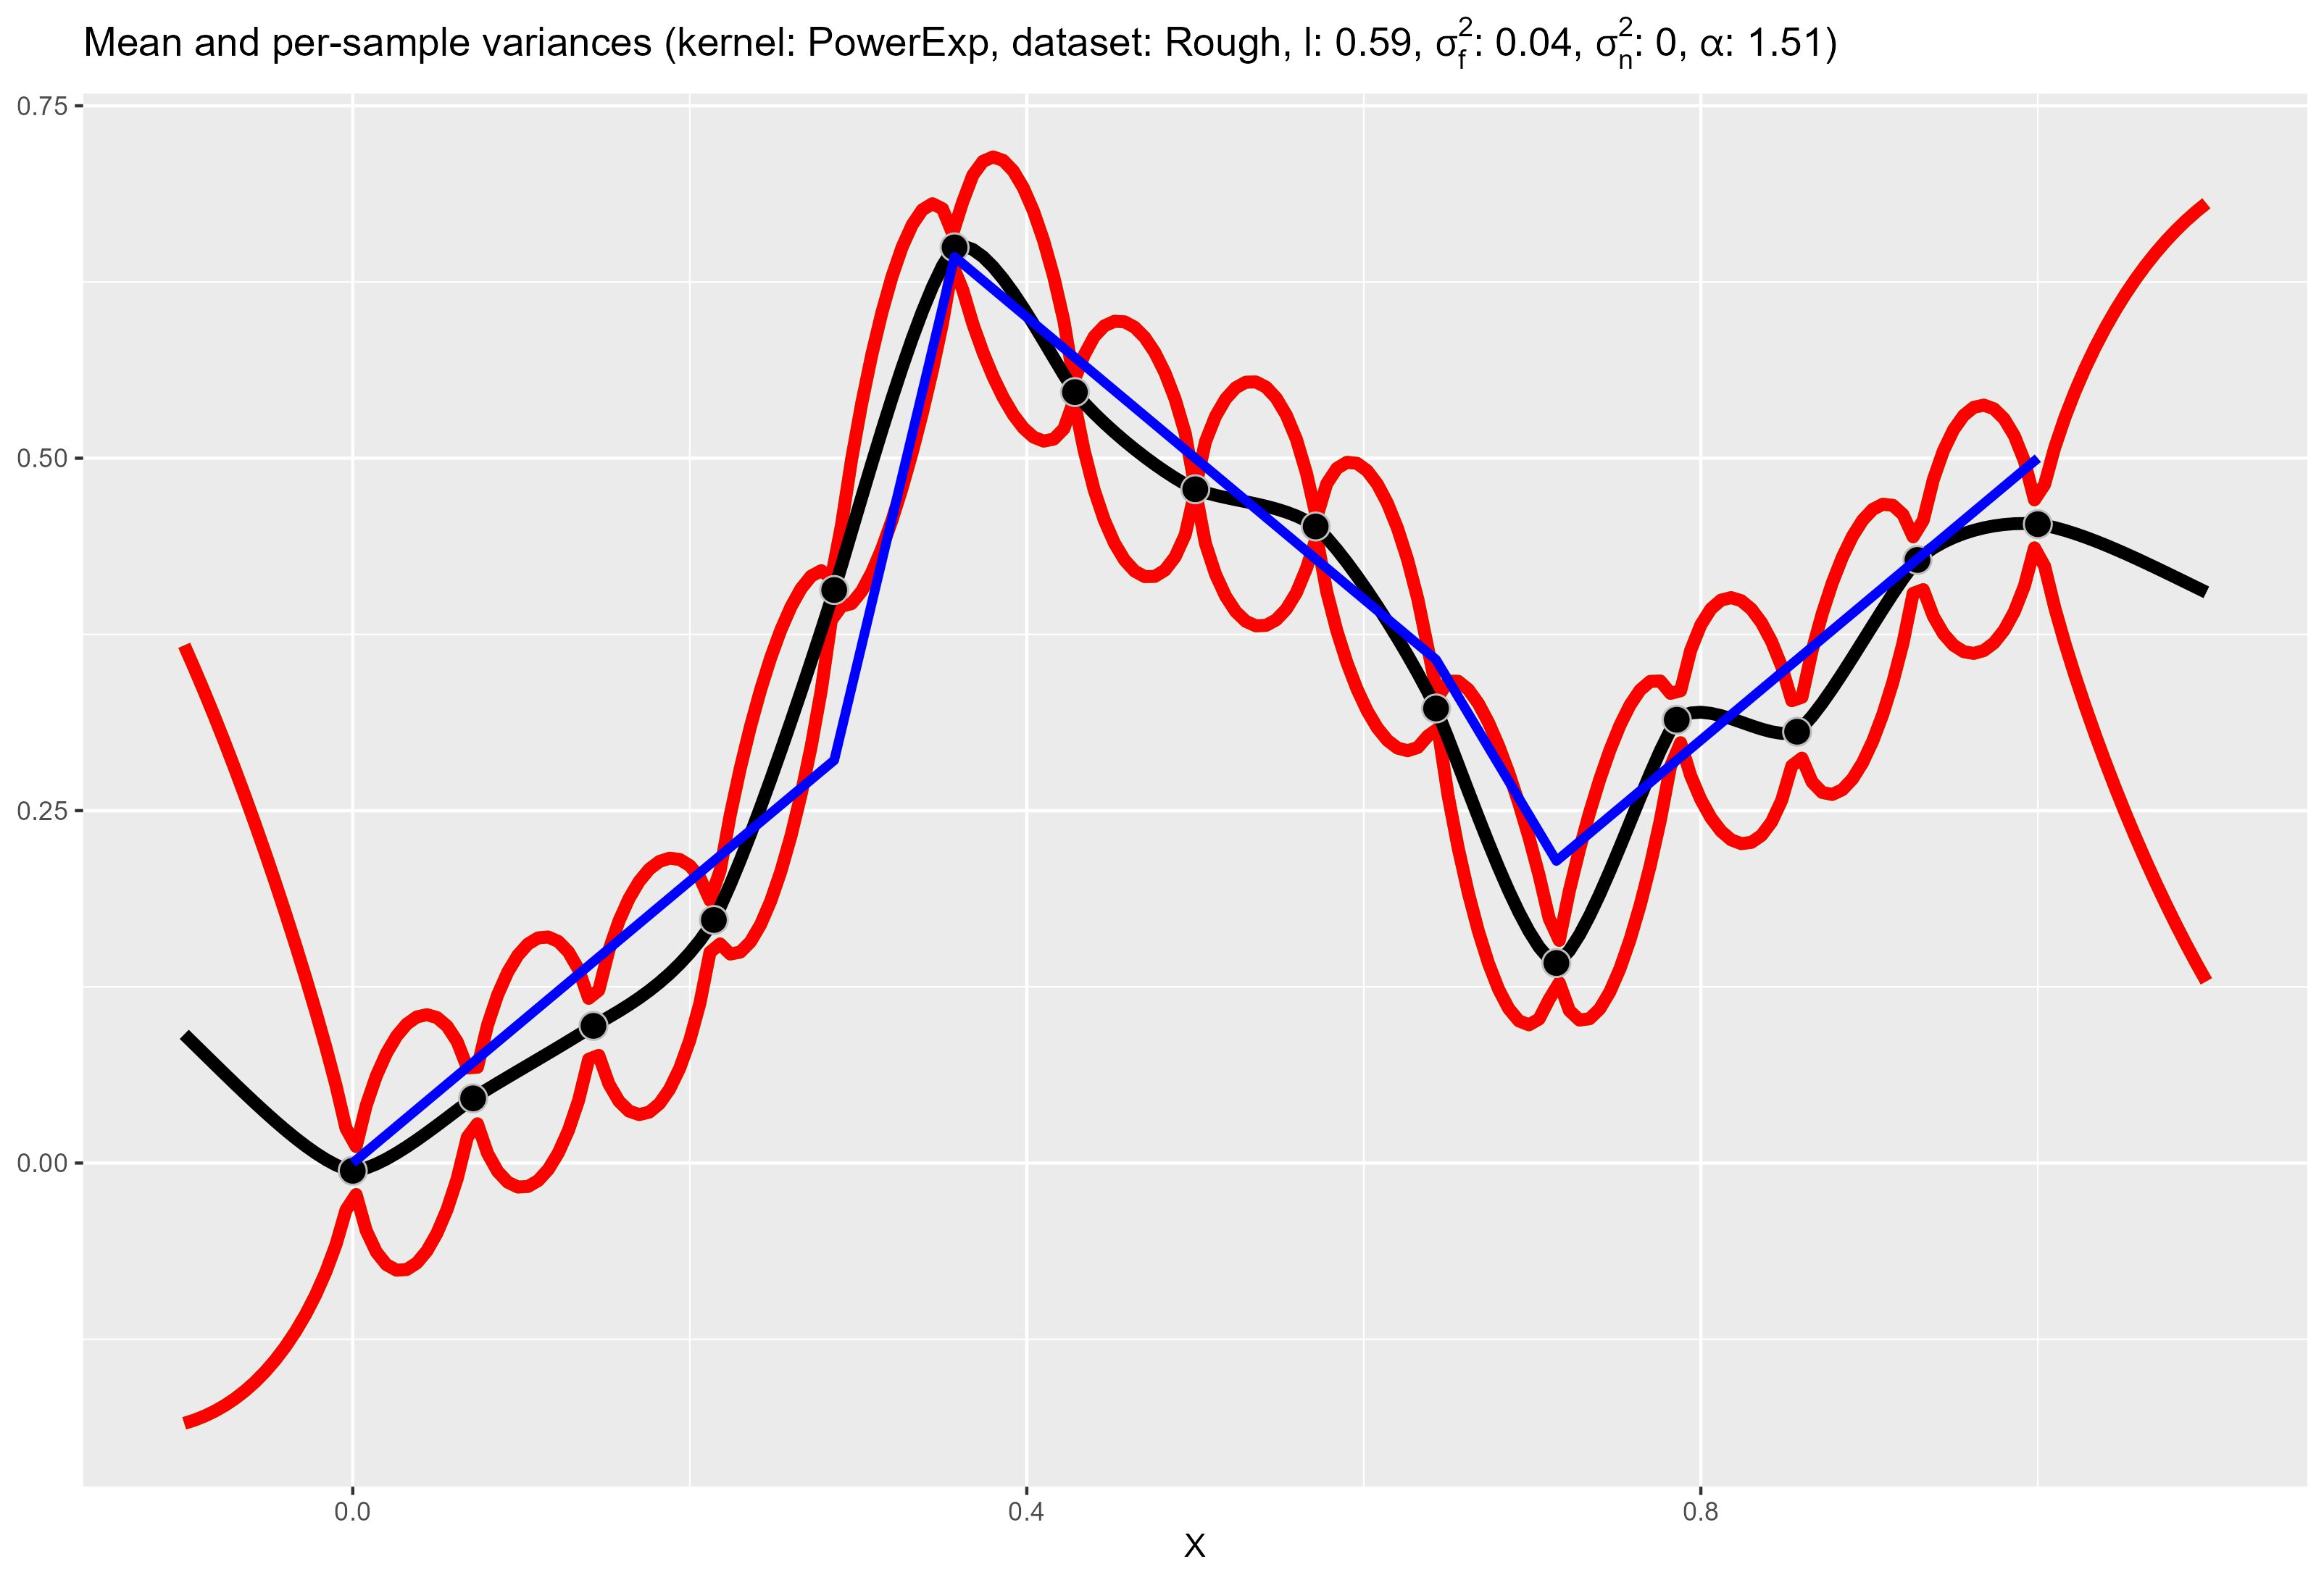
\includegraphics[height=0.5\textwidth]{covariance-functions/PowerExp_Rough_mean.png}
    \caption{
        Plot of the expected function draw and variances as before, using $\gamma$-exponential fitted to the rougher dataset. \\
    }
\end{figure}
$\gamma = 1.51$ has been selected by GauPro \cite{gaupro} via MLE, which produces a covariance function that is not differentiable at $|x - x'| = 0$. This is because the roughness of the data-generating function is too high for SE to capture, and the $\gamma$-exponential covariance function is able to adapt to this roughness. \\
        These variances appear not to collapse to zero at the training points. In fact, this is a graphical issue caused by the very rough functions that the $\gamma$-exponential covariance function produces. Unlike the functions drawn from an RQ-powered GP that remain close to the training points for some time before and after the training points, functions drawn from this distribution only remain close to the training points for a very short distance before diverging - a distance that is too small to be visible in this plot.

\begin{figure}[H]
    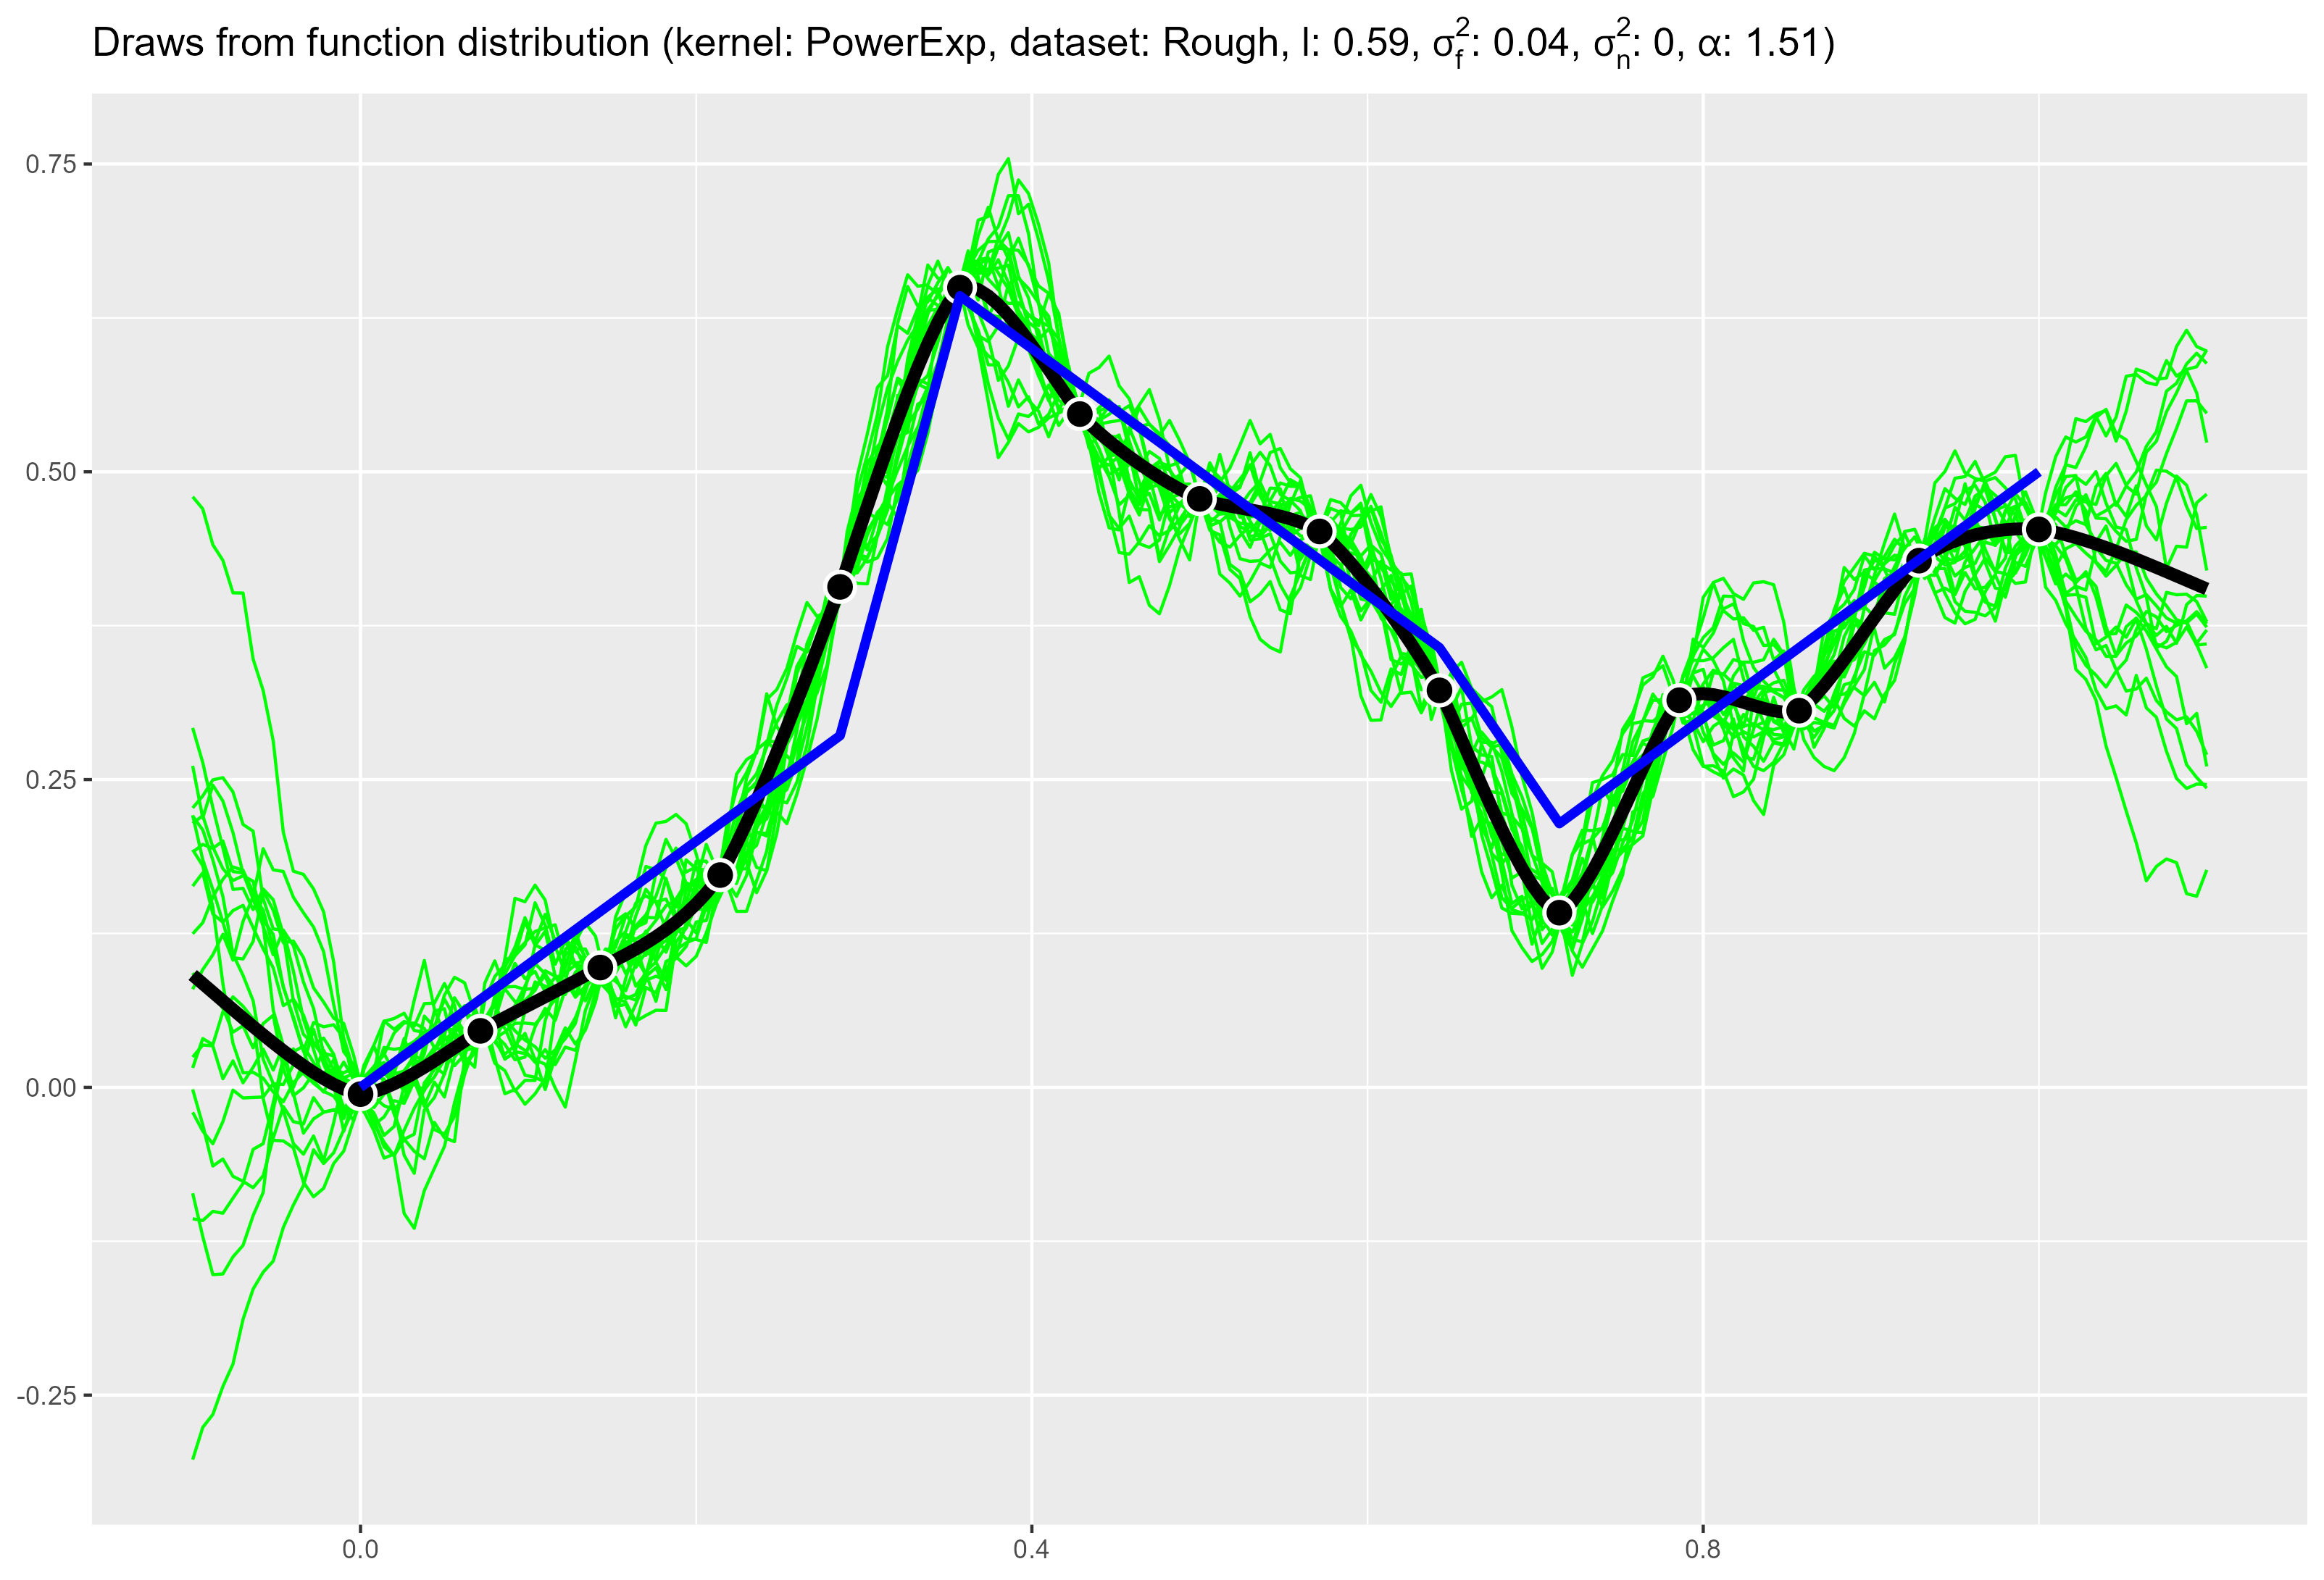
\includegraphics[height=0.5\textwidth]{covariance-functions/PowerExp_Rough_draws.png}
    \caption{
        Plots of some sample functions drawn from a GP as before, trained on the rough dataset using $\gamma$-exponential. \\
    }
\end{figure}
These function draws are much rougher than those drawn from RQ or SE thanks to their non-differentiability.

\paragraph{Exponential covariance function}
$\gamma = 1$ produces the exponential covariance function:
\begin{equation*}
    k(X,X') = \exp \left(-\frac{|X - X'|}{l} \right)
\end{equation*}
Restating:
\begin{equation*}
    k(X, X') = a \exp\left(-c |X - X'|\right)
\end{equation*}
    Setting $a = 1$ and $c = \frac{1}{l}$ recovers our familiar exponential kernel \ref{eq:exp_kernel}. This form relates to the Ornstein-Uhlenbeck \cite{orny} stochastic differential equation (SDE):
\begin{equation*}
    dX_t = -\lambda X_t dt + \sqrt{2\lambda} dW_t
\end{equation*}
    This SDE has a unique stationary Gaussian solution \cite{orny} with a covariance equal to that of the exponential covariance function where $a = \sigma^2$ and $c = \lambda$:
\begin{equation*}
    \begin{aligned}
        \mathbb{E}[X_t] = 0 \\
        \text{Cov}(X_t, X_s) = \sigma^2 \exp \left( -\lambda |t - s| \right)
    \end{aligned}
\end{equation*}
    Because this SDE is of order one, the OU process is Gauss-Markovian, meaning that the future state of the process only depends on the current state $X_t$ and not on any previous states $X_{t-1}$. Higher order SDEs with integer order $m$ produce Matern covariance functions with $\nu = m - \frac{1}{2}$.

\begin{figure}[H]
    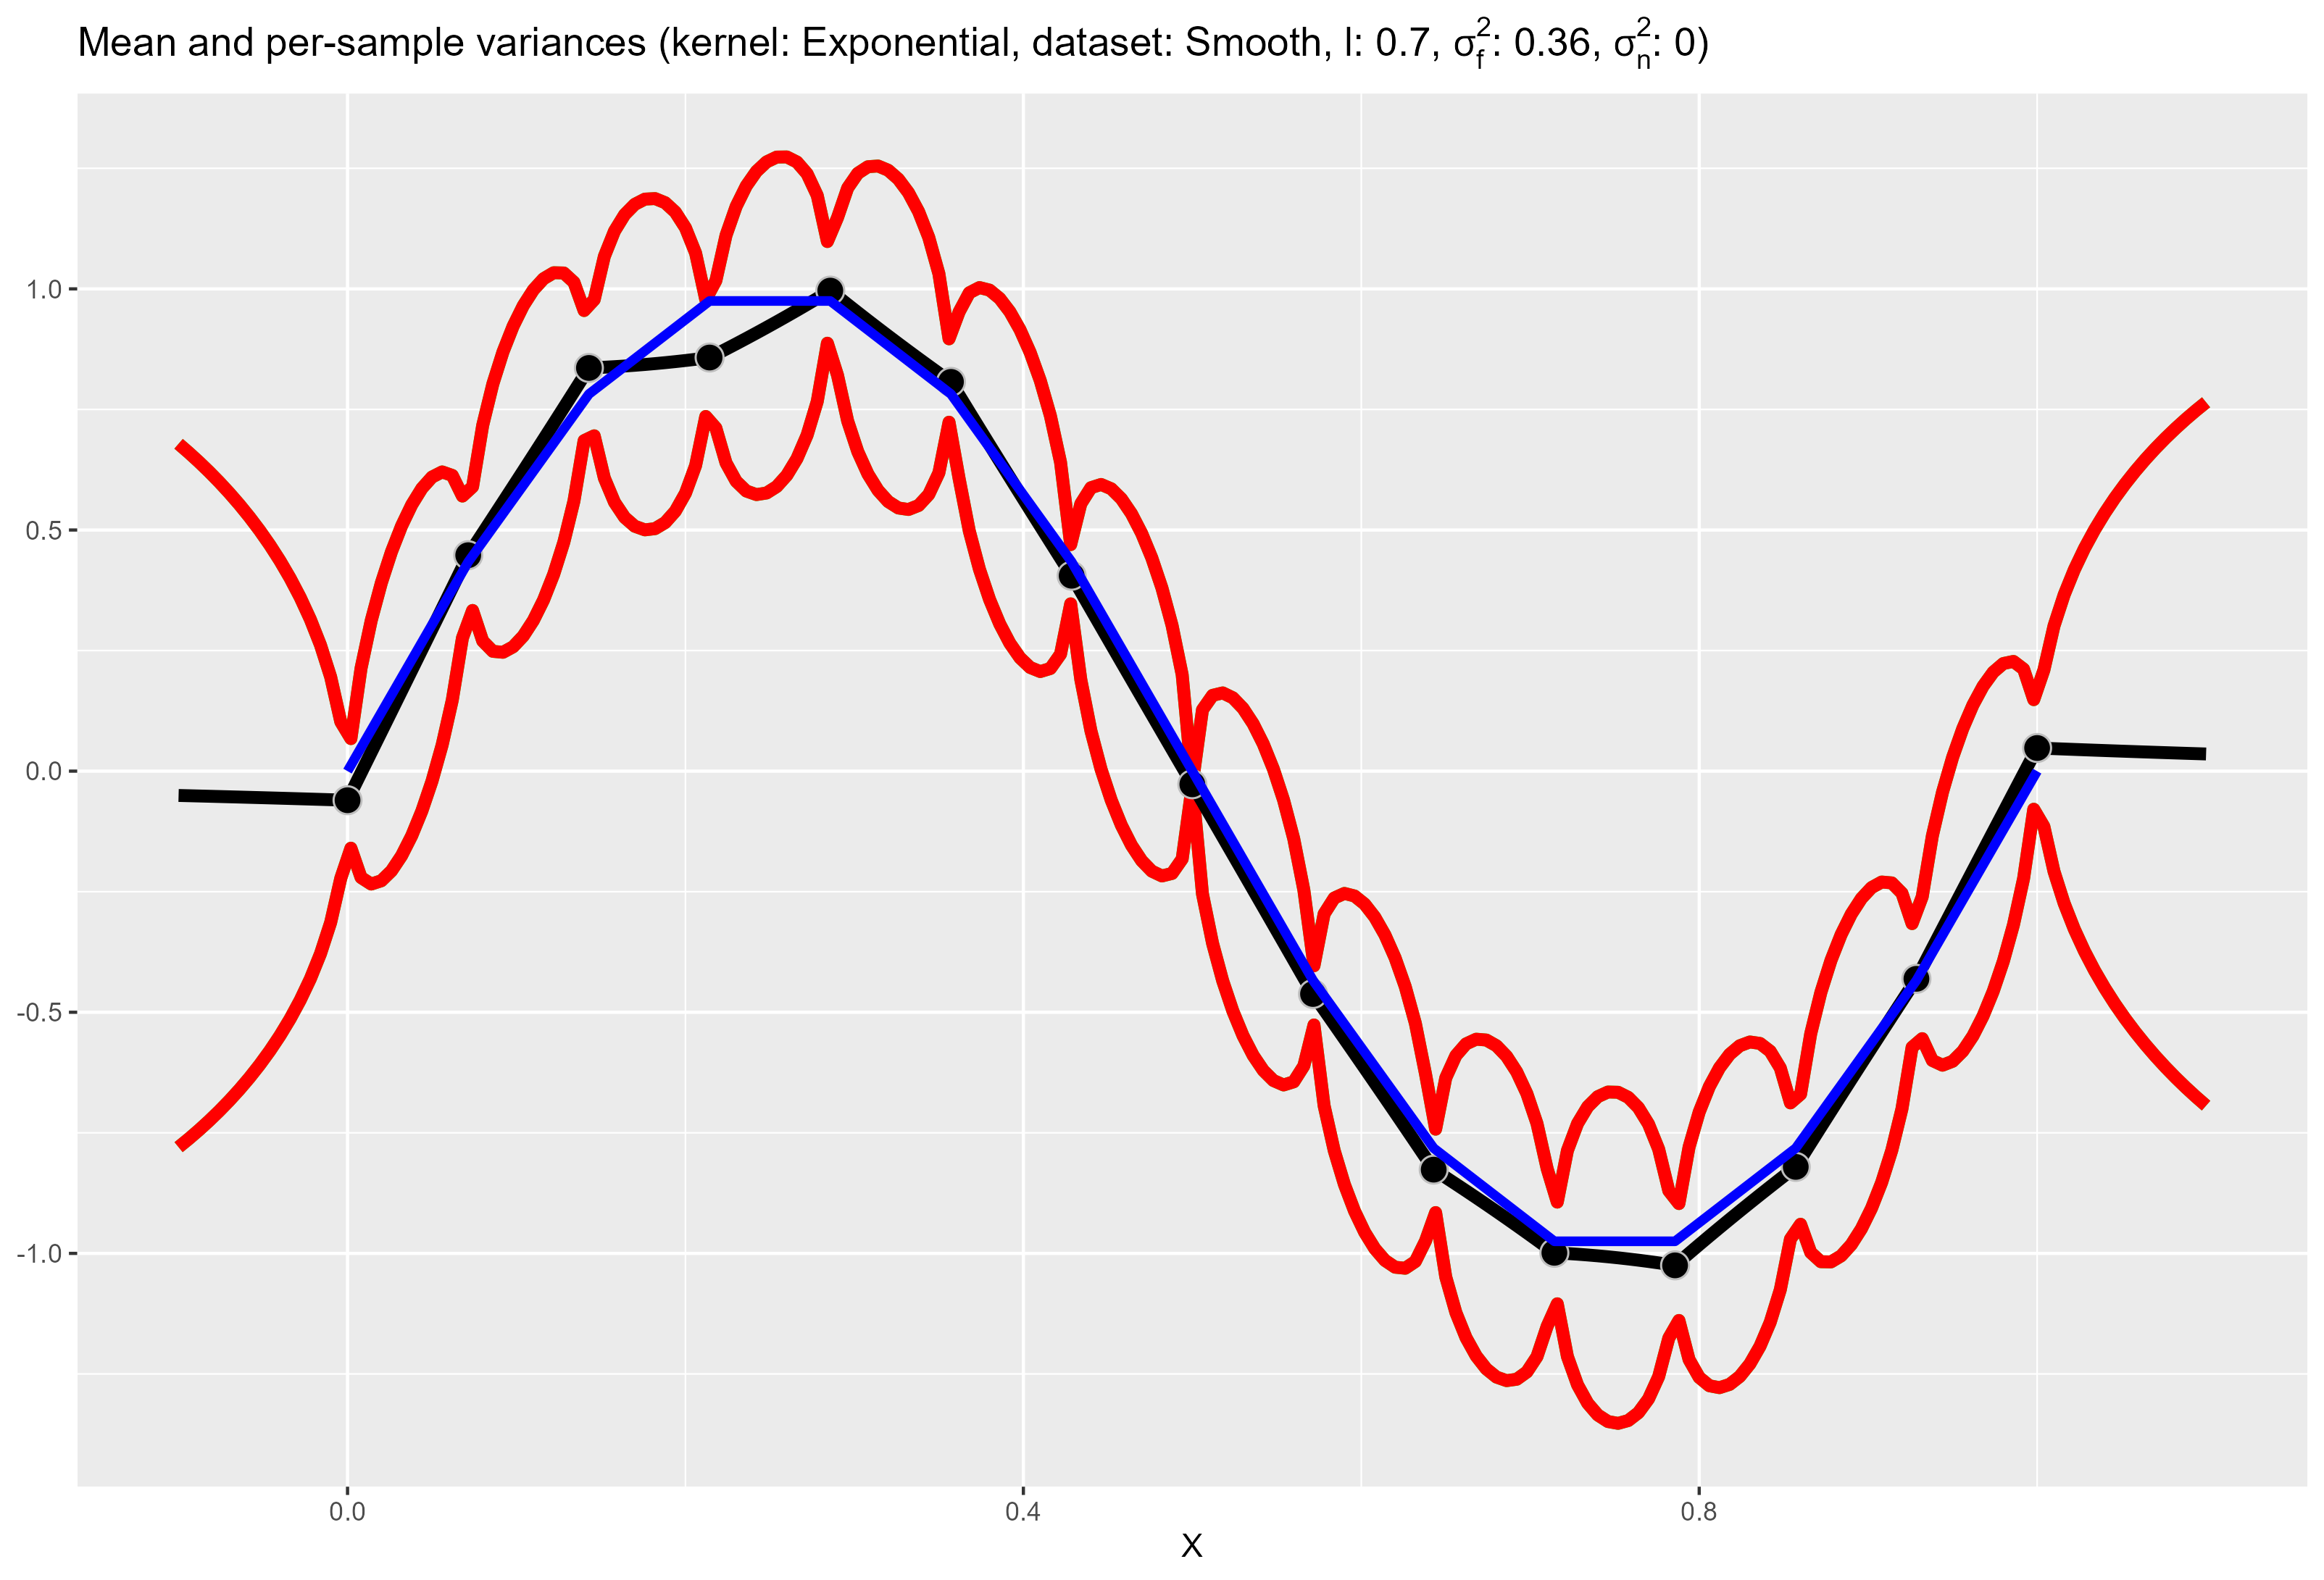
\includegraphics[height=0.5\textwidth]{covariance-functions/Exponential_Smooth_mean.png}
    \caption{
        Plot of the expected function draw and variances as before, using exponential fitted to the smooth sin wave dataset. \\
    }
\end{figure}
The expected function draw is practically a straight line connecting each data point, as the exponential covariance function is not smooth enough to capture the sin wave. The graphical issue observed in $\gamma$-exponential is more pronounced here, with the variances barely approaching zero as $x_*$ approach a training point.

\begin{figure}[H]
    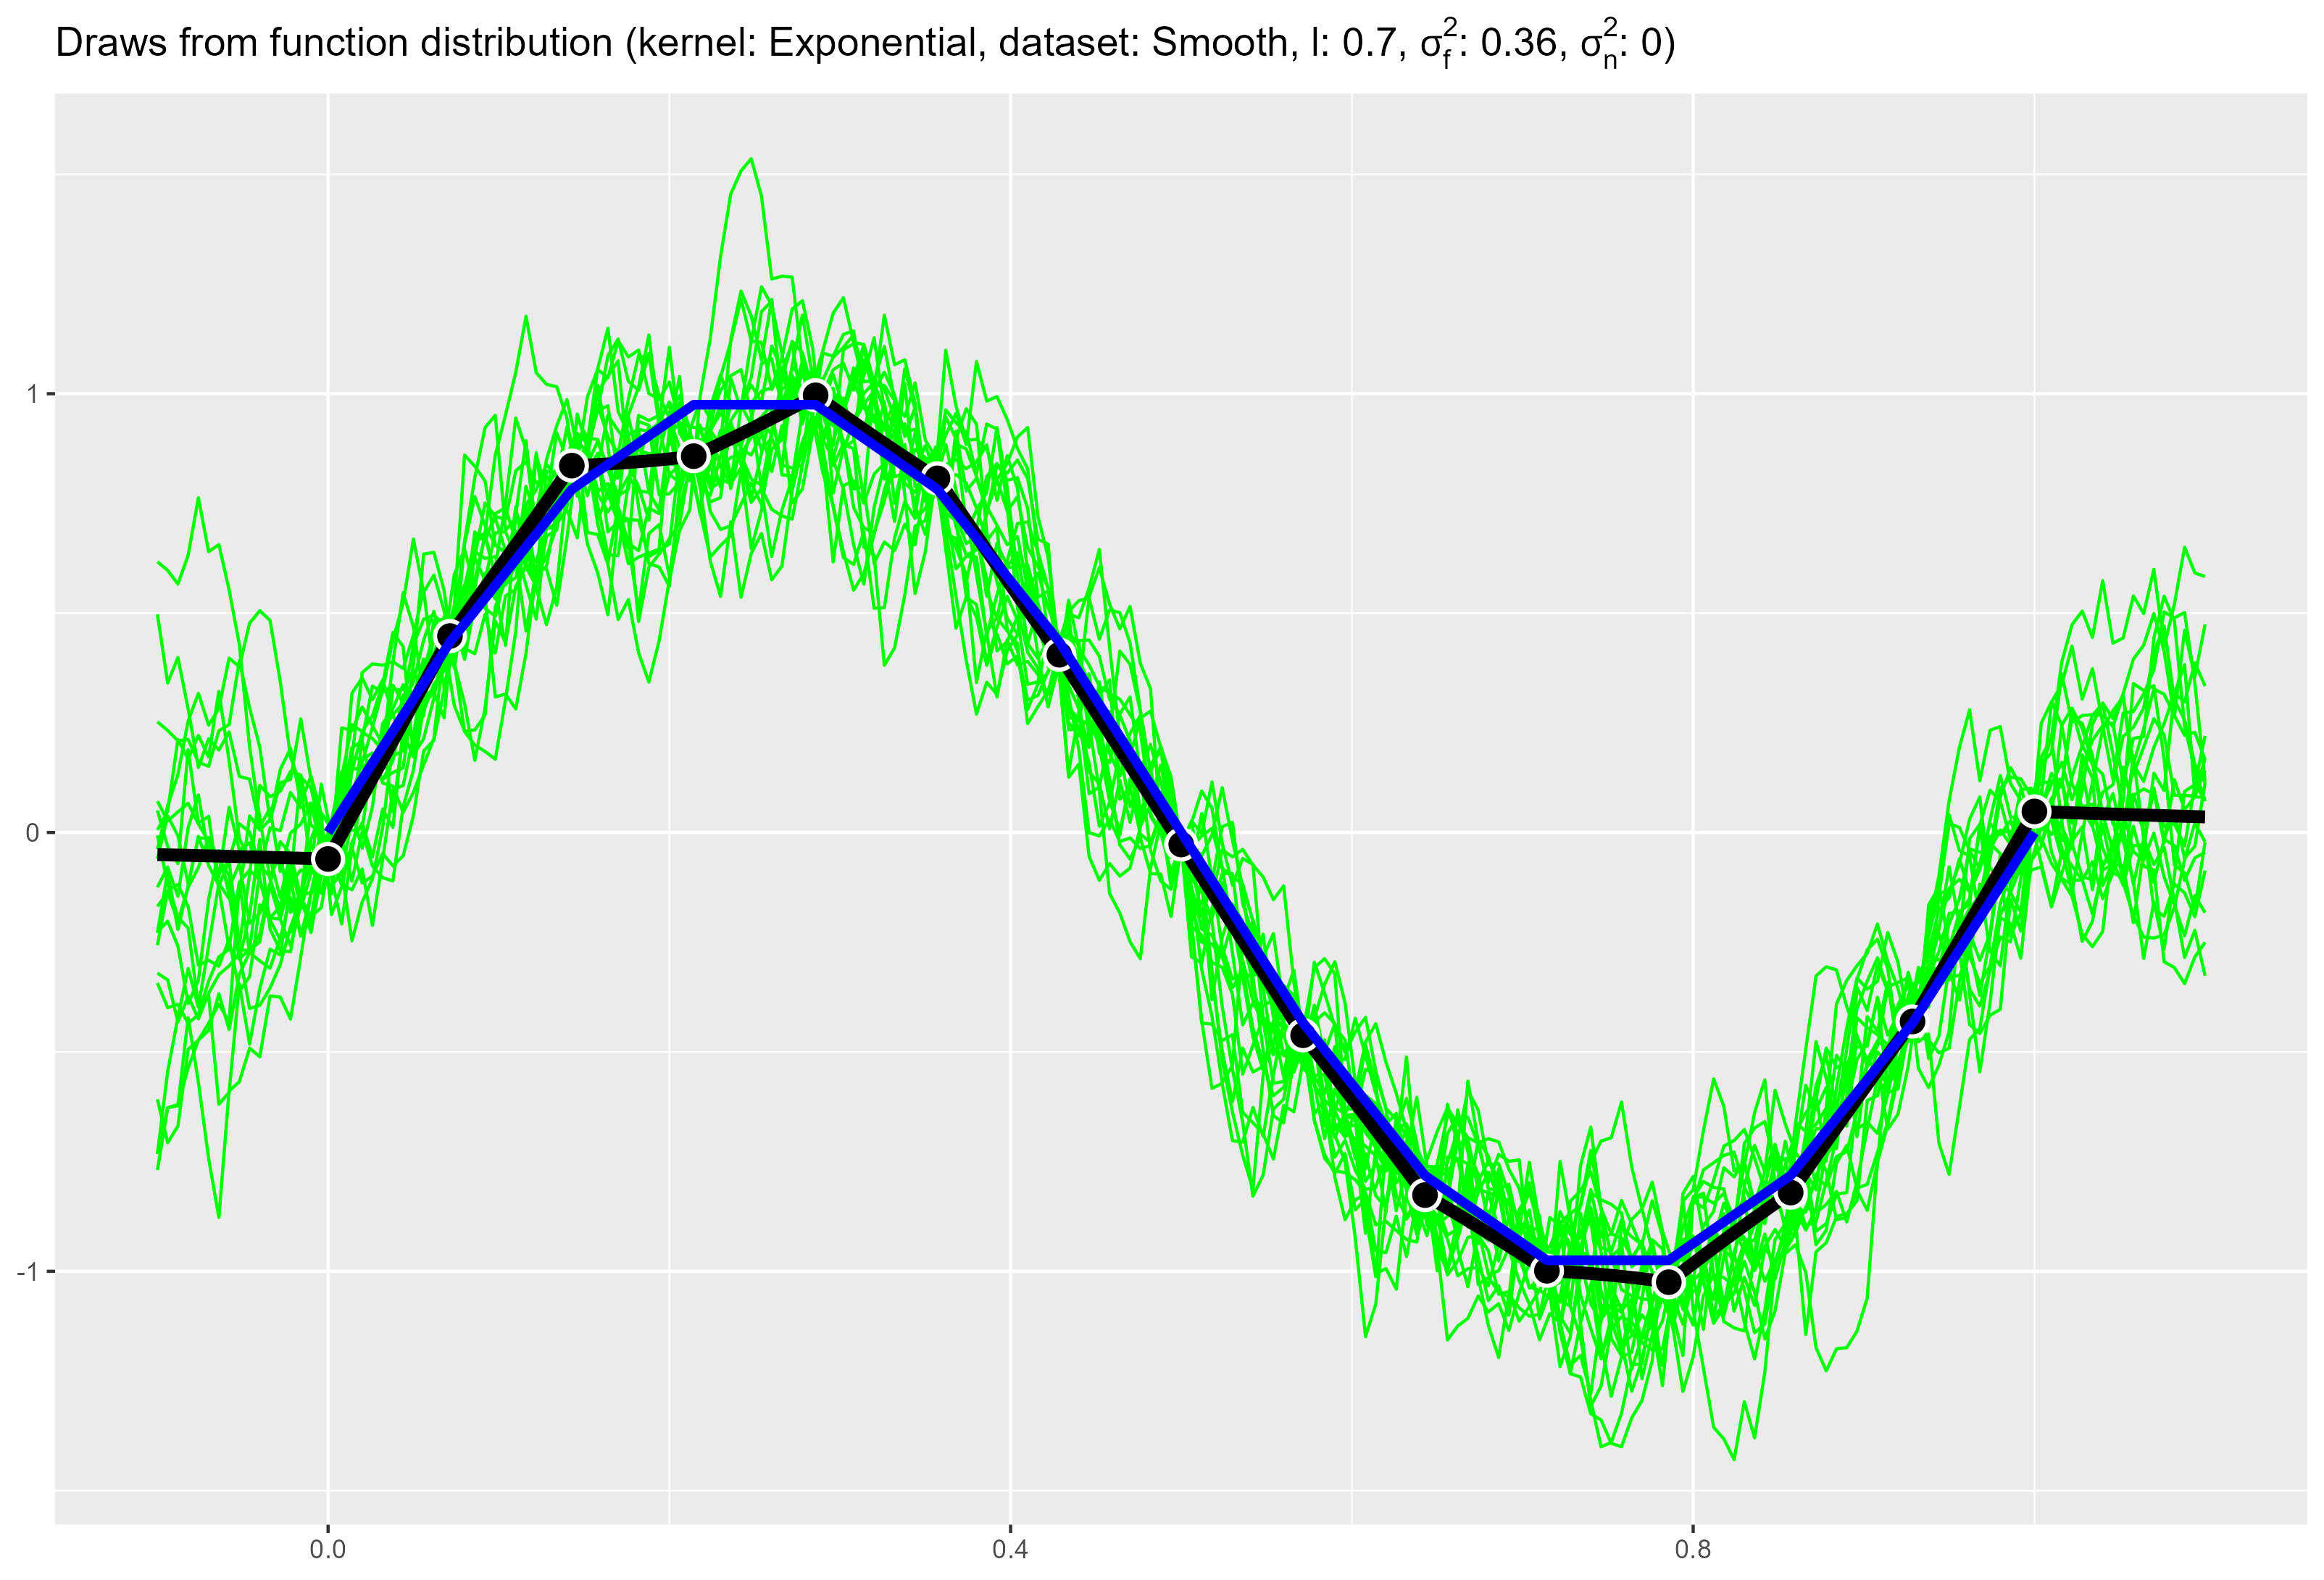
\includegraphics[height=0.5\textwidth]{covariance-functions/Exponential_Smooth_draws.png}
    \caption{
        Plots of some sample functions drawn from a GP as before, trained on the smooth dataset using exponential. \\
    }
\end{figure}
These function draws are effectively white noise that collapses at training points.

\begin{figure}[H]
    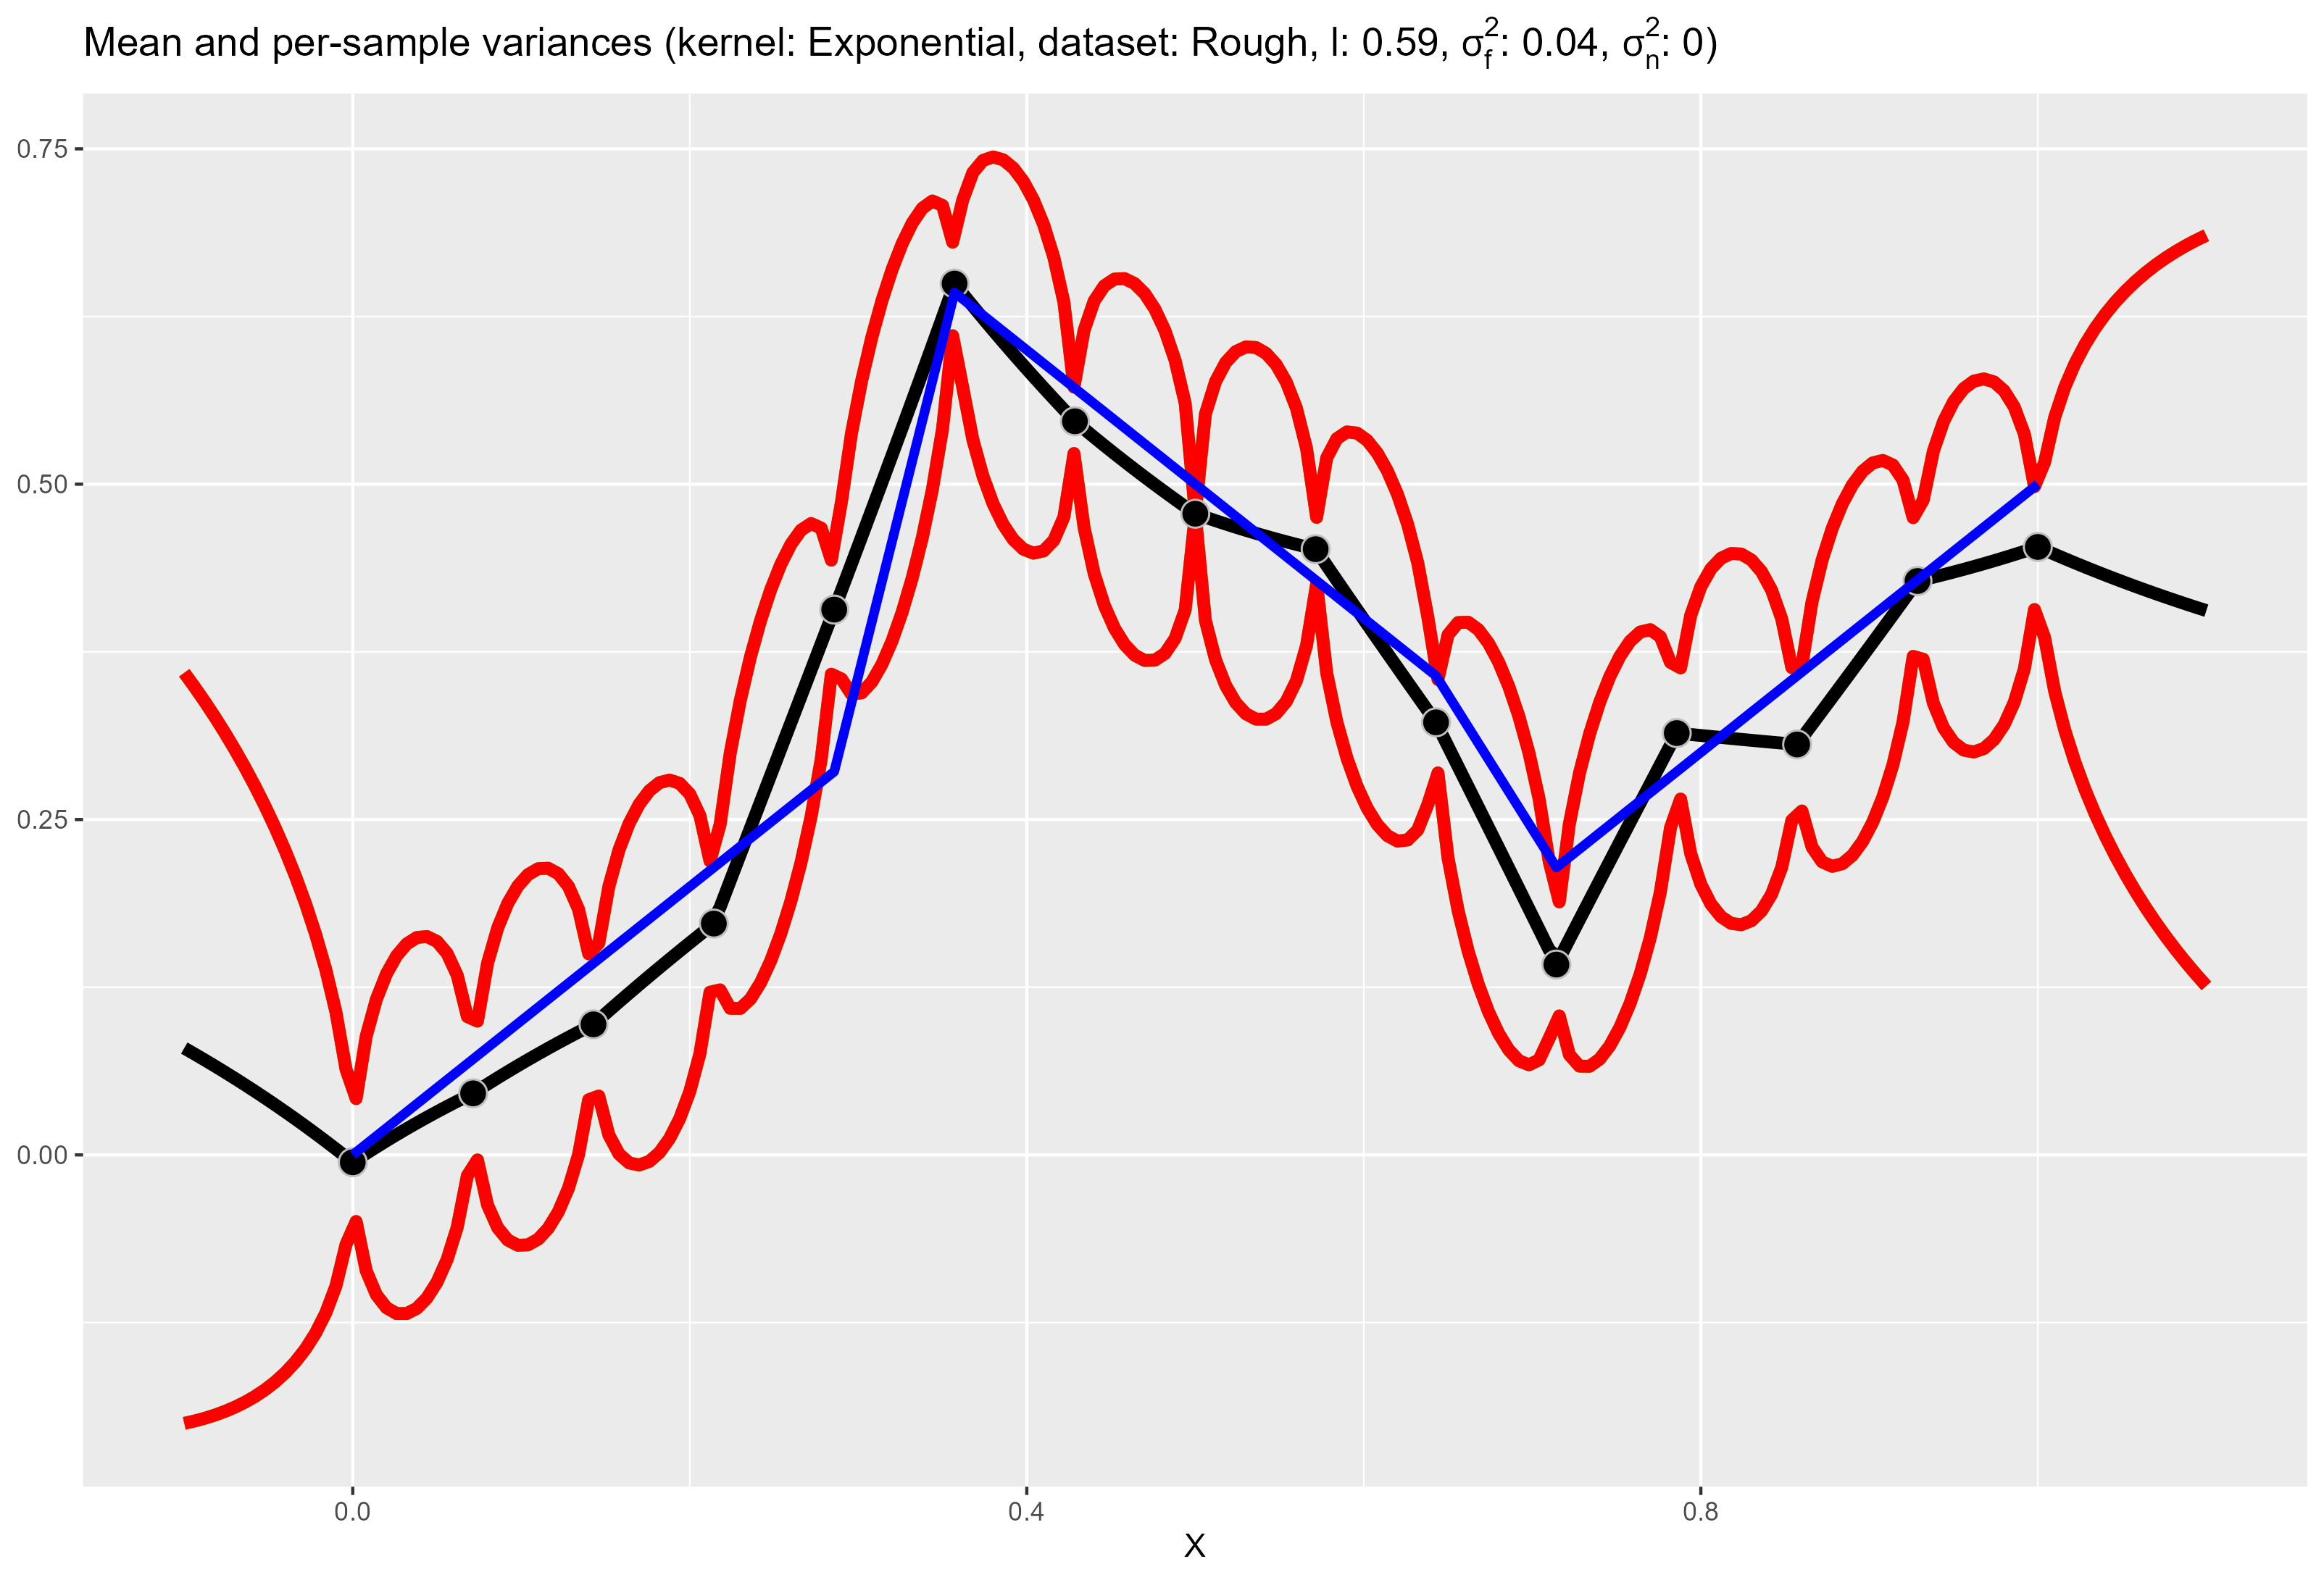
\includegraphics[height=0.5\textwidth]{covariance-functions/Exponential_Rough_mean.png}
    \caption{
        Plot of the expected function draw and variances as before, using exponential fitted to the rougher dataset.
    }
\end{figure}
The behaviour of GPs using the exponential covariance function is invariant to the data it is trained on - as with the smooth dataset, the expected function draw is a straight line connecting each data point, and the variances barely approach zero as $x_*$ approaches a training point. 
% Exponential: Equivalent to Matern 1/2. Assumes no differentiability. \cite{gaupro}


\subsubsection{Matern-class}
The $\gamma$-exponential generalisation is not useful due to its brittleness - it can only produce two covariance functions representing the extremes of the smoothness-roughness scale. The Matern class of covariance functions addresses this by introducing a parameter $\nu > 0$ that controls the smoothness of the function. The Matern class is defined as:
\begin{equation*}
    k(X,X') = \frac{2^{1 - \nu}}{\Gamma(\nu)}\left(\frac{\sqrt{2\nu}|X - X'|}{l}\right)^{\nu}K_{\nu}\left(\frac{\sqrt{2\nu}|X - X'|}{l}\right)
\end{equation*}

$l$ is our familiar length scale hyperparameter, and $K_{\nu}$ is a modified Bessel function. This class has a spectral density:
\begin{equation} \label{eq:matern_spectral}
    S(\omega) = \frac{2^D \pi^{D/2} \Gamma(\nu + D/2) (2\nu)^\nu}{\Gamma(\nu) l^{2\nu}} \left( \frac{2\nu}{l^2} + 4 \pi^2 s^2 \right)^{-(\nu + D/2)} 
\end{equation}
A Gaussian process using a Matern class kernel is $k$-times MS differentiable if and only if $\nu > k$. 

Using half-integers, i.e. $\nu = p + 1/2$ where $p$ is a non-negative integer, the covariance function becomes a product of a polynomial and an exponential:
\begin{equation*}
    k_{\nu = p + 1/2}(X,X') = \exp \left(- \frac{\sqrt{2\nu}|X - X'|}{l} \right) \frac{\Gamma(p+1)}{\Gamma(2p+1)} \sum_{i=0}^p \frac{(p + i)!}{i!(p-i)!} \left( \frac{\sqrt{8\nu r}}{l} \right)^{p-i}
\end{equation*}
As $\nu \to \infty$, the Matern covariance function approaches the SE covariance function. $\nu = 1/2$ yields the exponential covariance function, and $\nu \geq 7/2$ produces functions that are as smooth as SE, leaving us with two cases of interest: $\nu = 3/2$ and $\nu = 5/2$.

\paragraph{Matern 3/2}
$\nu = 3/2$ produces the following covariance function:
\begin{equation} \label{eq:matern-32}
    k_{3/2}(X,X') = \left(1 + \frac{\sqrt{3}|X - X'|}{l} \right) \exp \left(-\frac{\sqrt{3}|X - X'|}{l} \right)
\end{equation}
3/2 is one-time MS differentiable, leading to much rougher functions than SE but smoother than exponential.

\begin{figure}[H]
    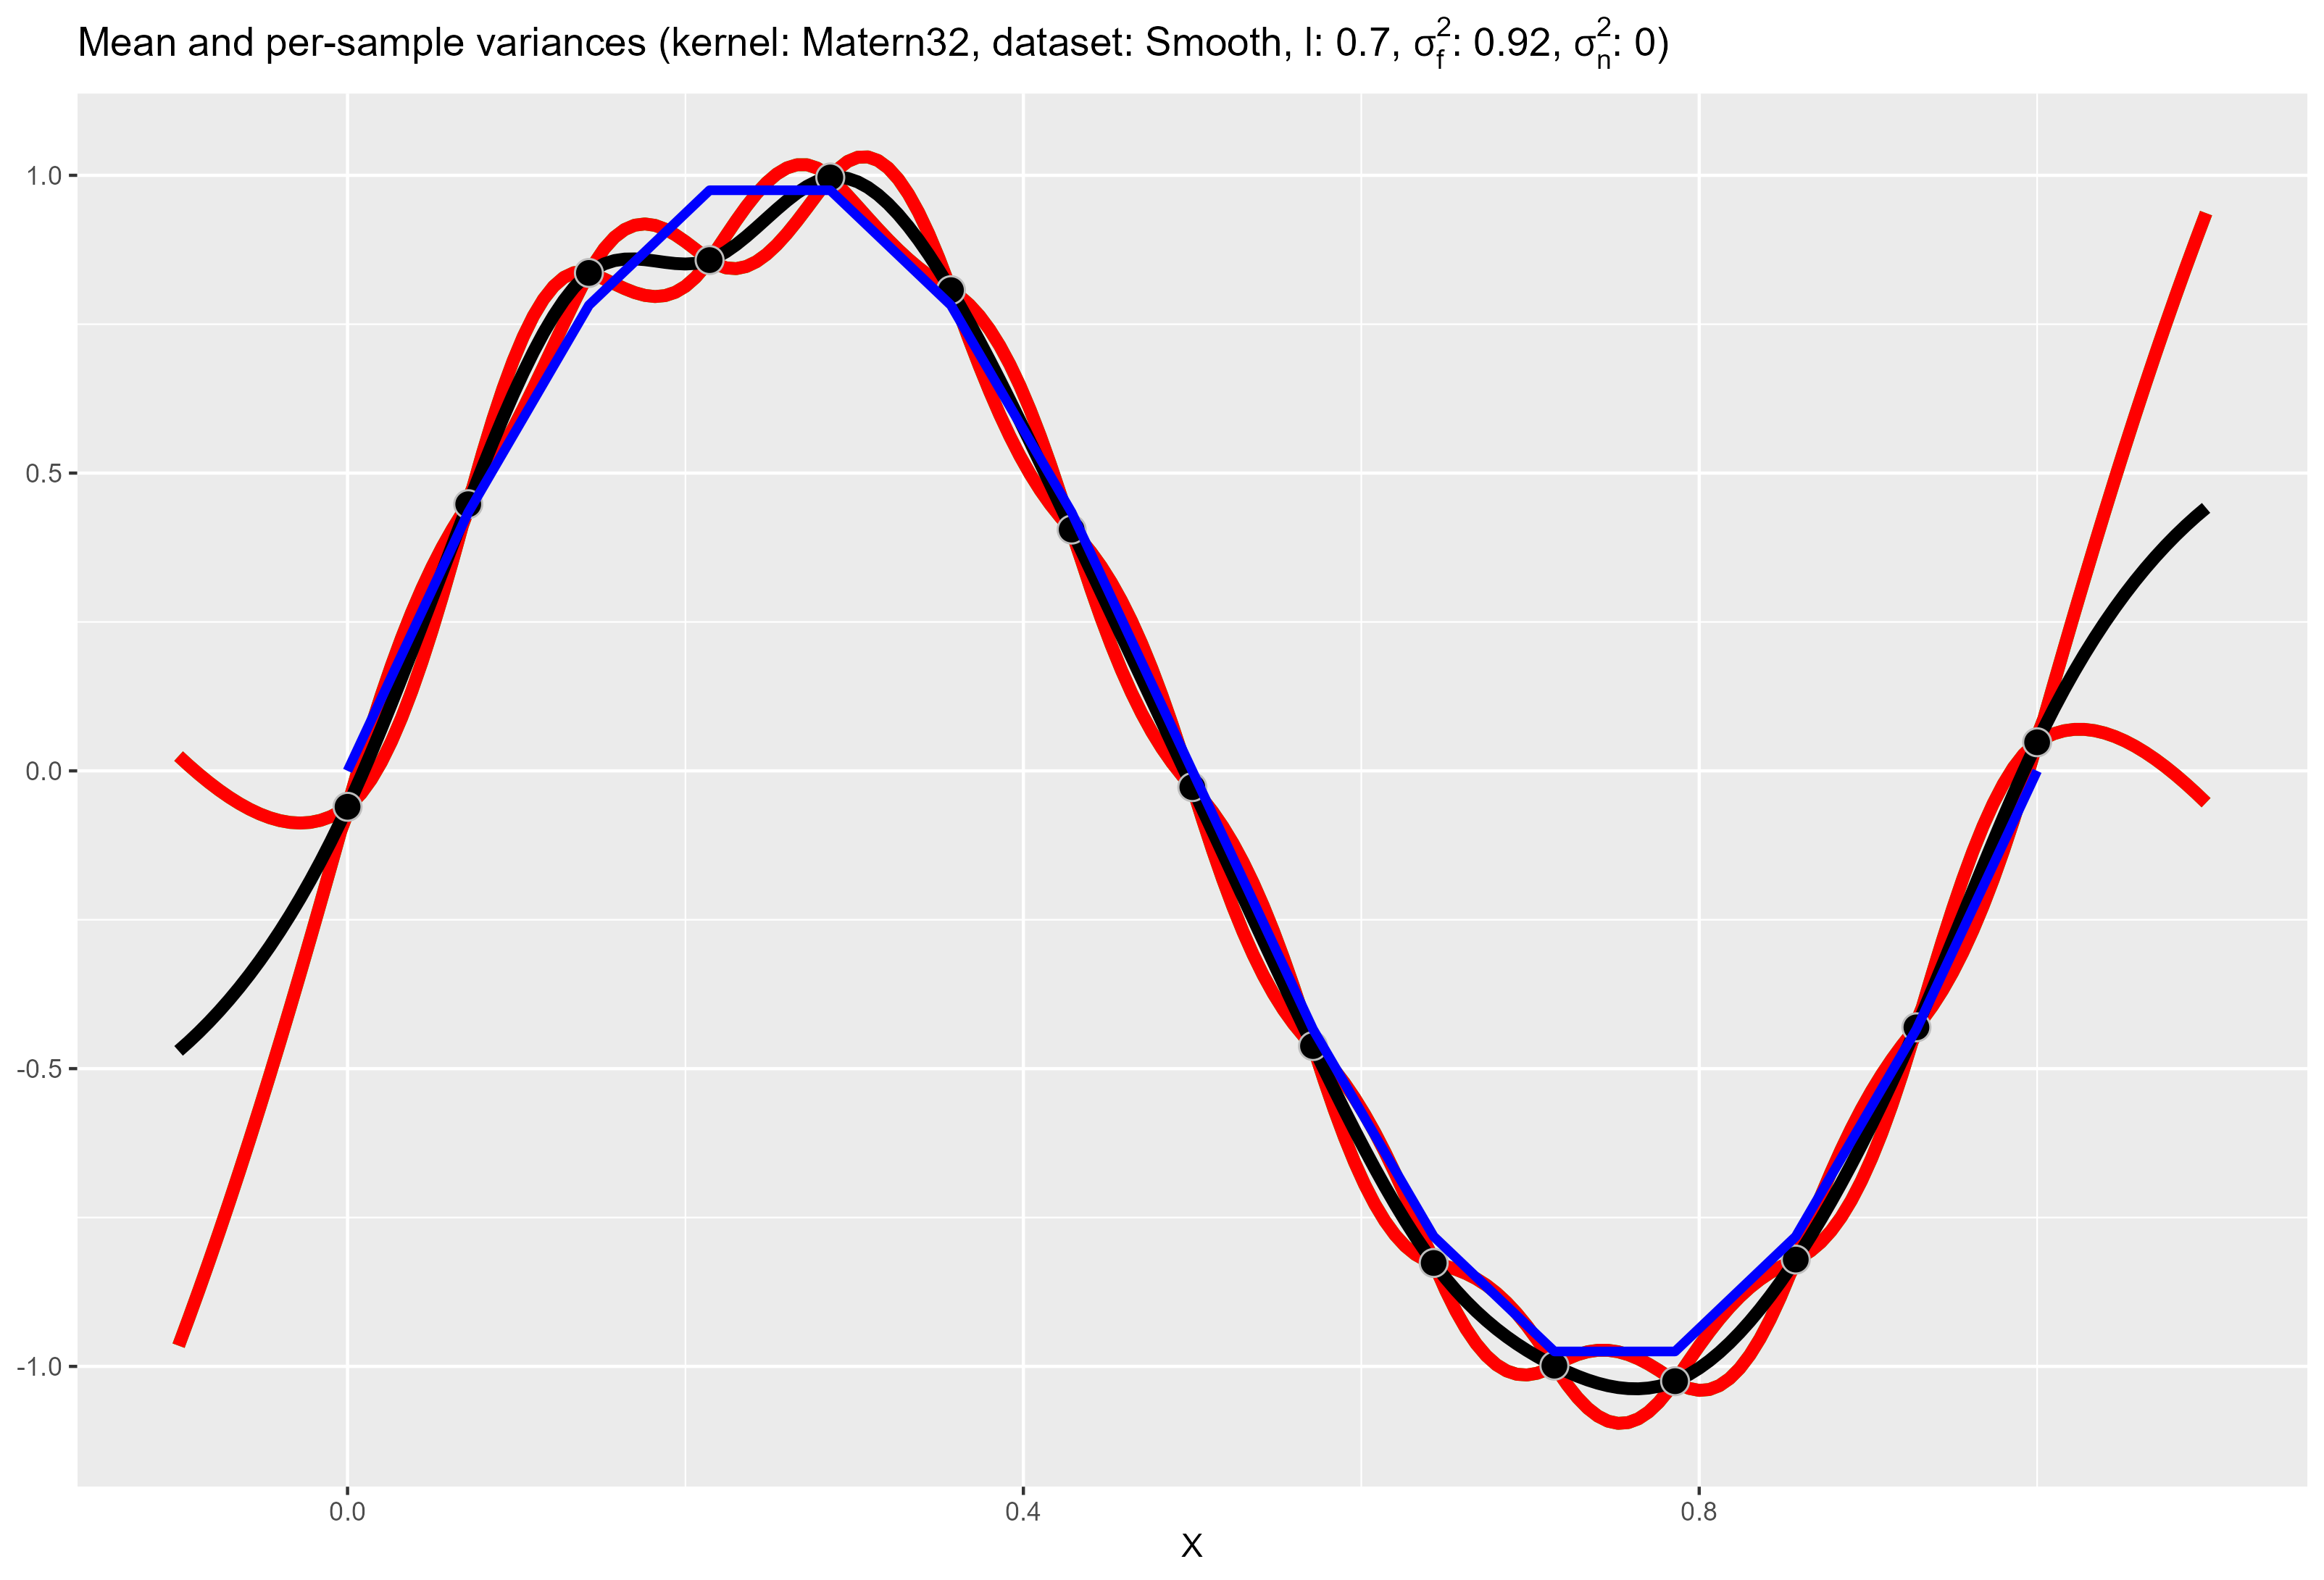
\includegraphics[height=0.5\textwidth]{covariance-functions/Matern32_Smooth_mean.png}
    \caption{
        Plot of the expected function draw and variances as before, using Matern 3/2 fitted to the smooth sin wave dataset.
    }
\end{figure}
This GP's expected function draw goes directly to the training points, similar to the behaviour of the exponential covariance function. Unlike the exponential covariance function, the one-time MS differentiability constraint on the sample functions restricts the sample functions from resembling white noise, which produces narrower variances closer to the expected draw.

\begin{figure}[H]
    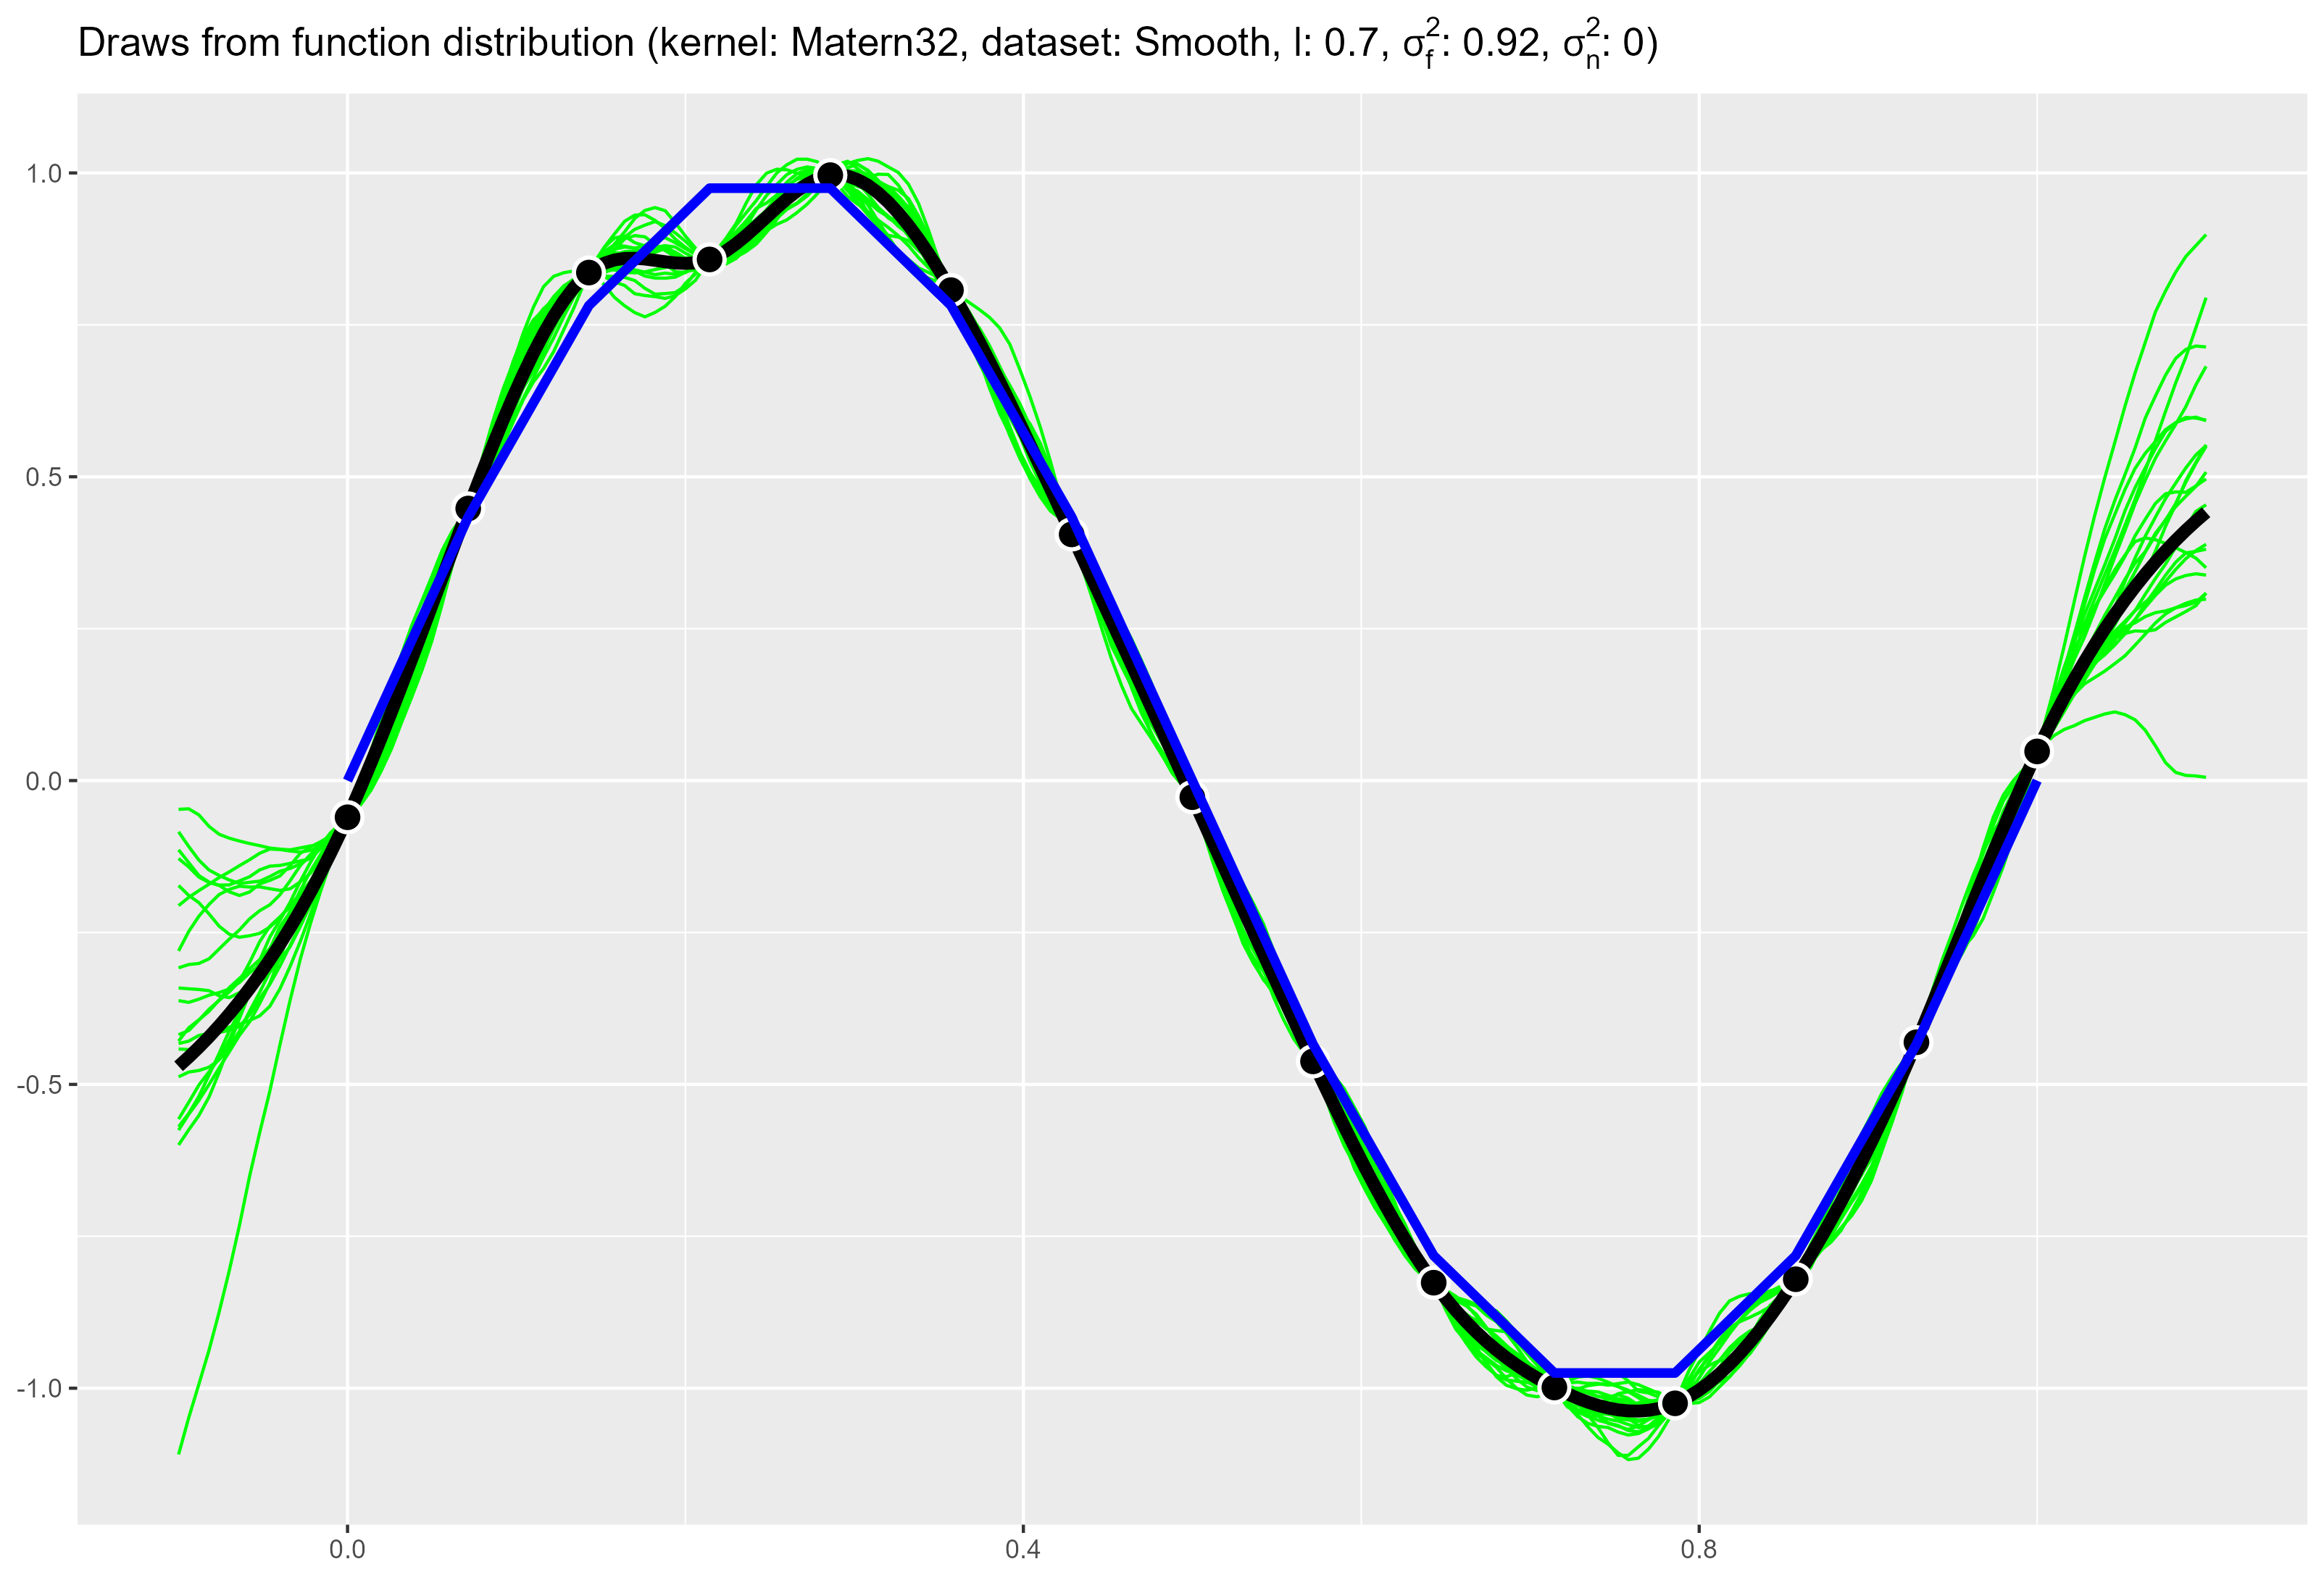
\includegraphics[height=0.5\textwidth]{covariance-functions/Matern32_Smooth_draws.png}
    \caption{
        Plots of some sample functions drawn from a GP as before, trained on the smooth dataset using Matern 3/2.
    }
\end{figure}
These function draws are much smoother than those drawn from the exponential covariance function.

\begin{figure}[H]
    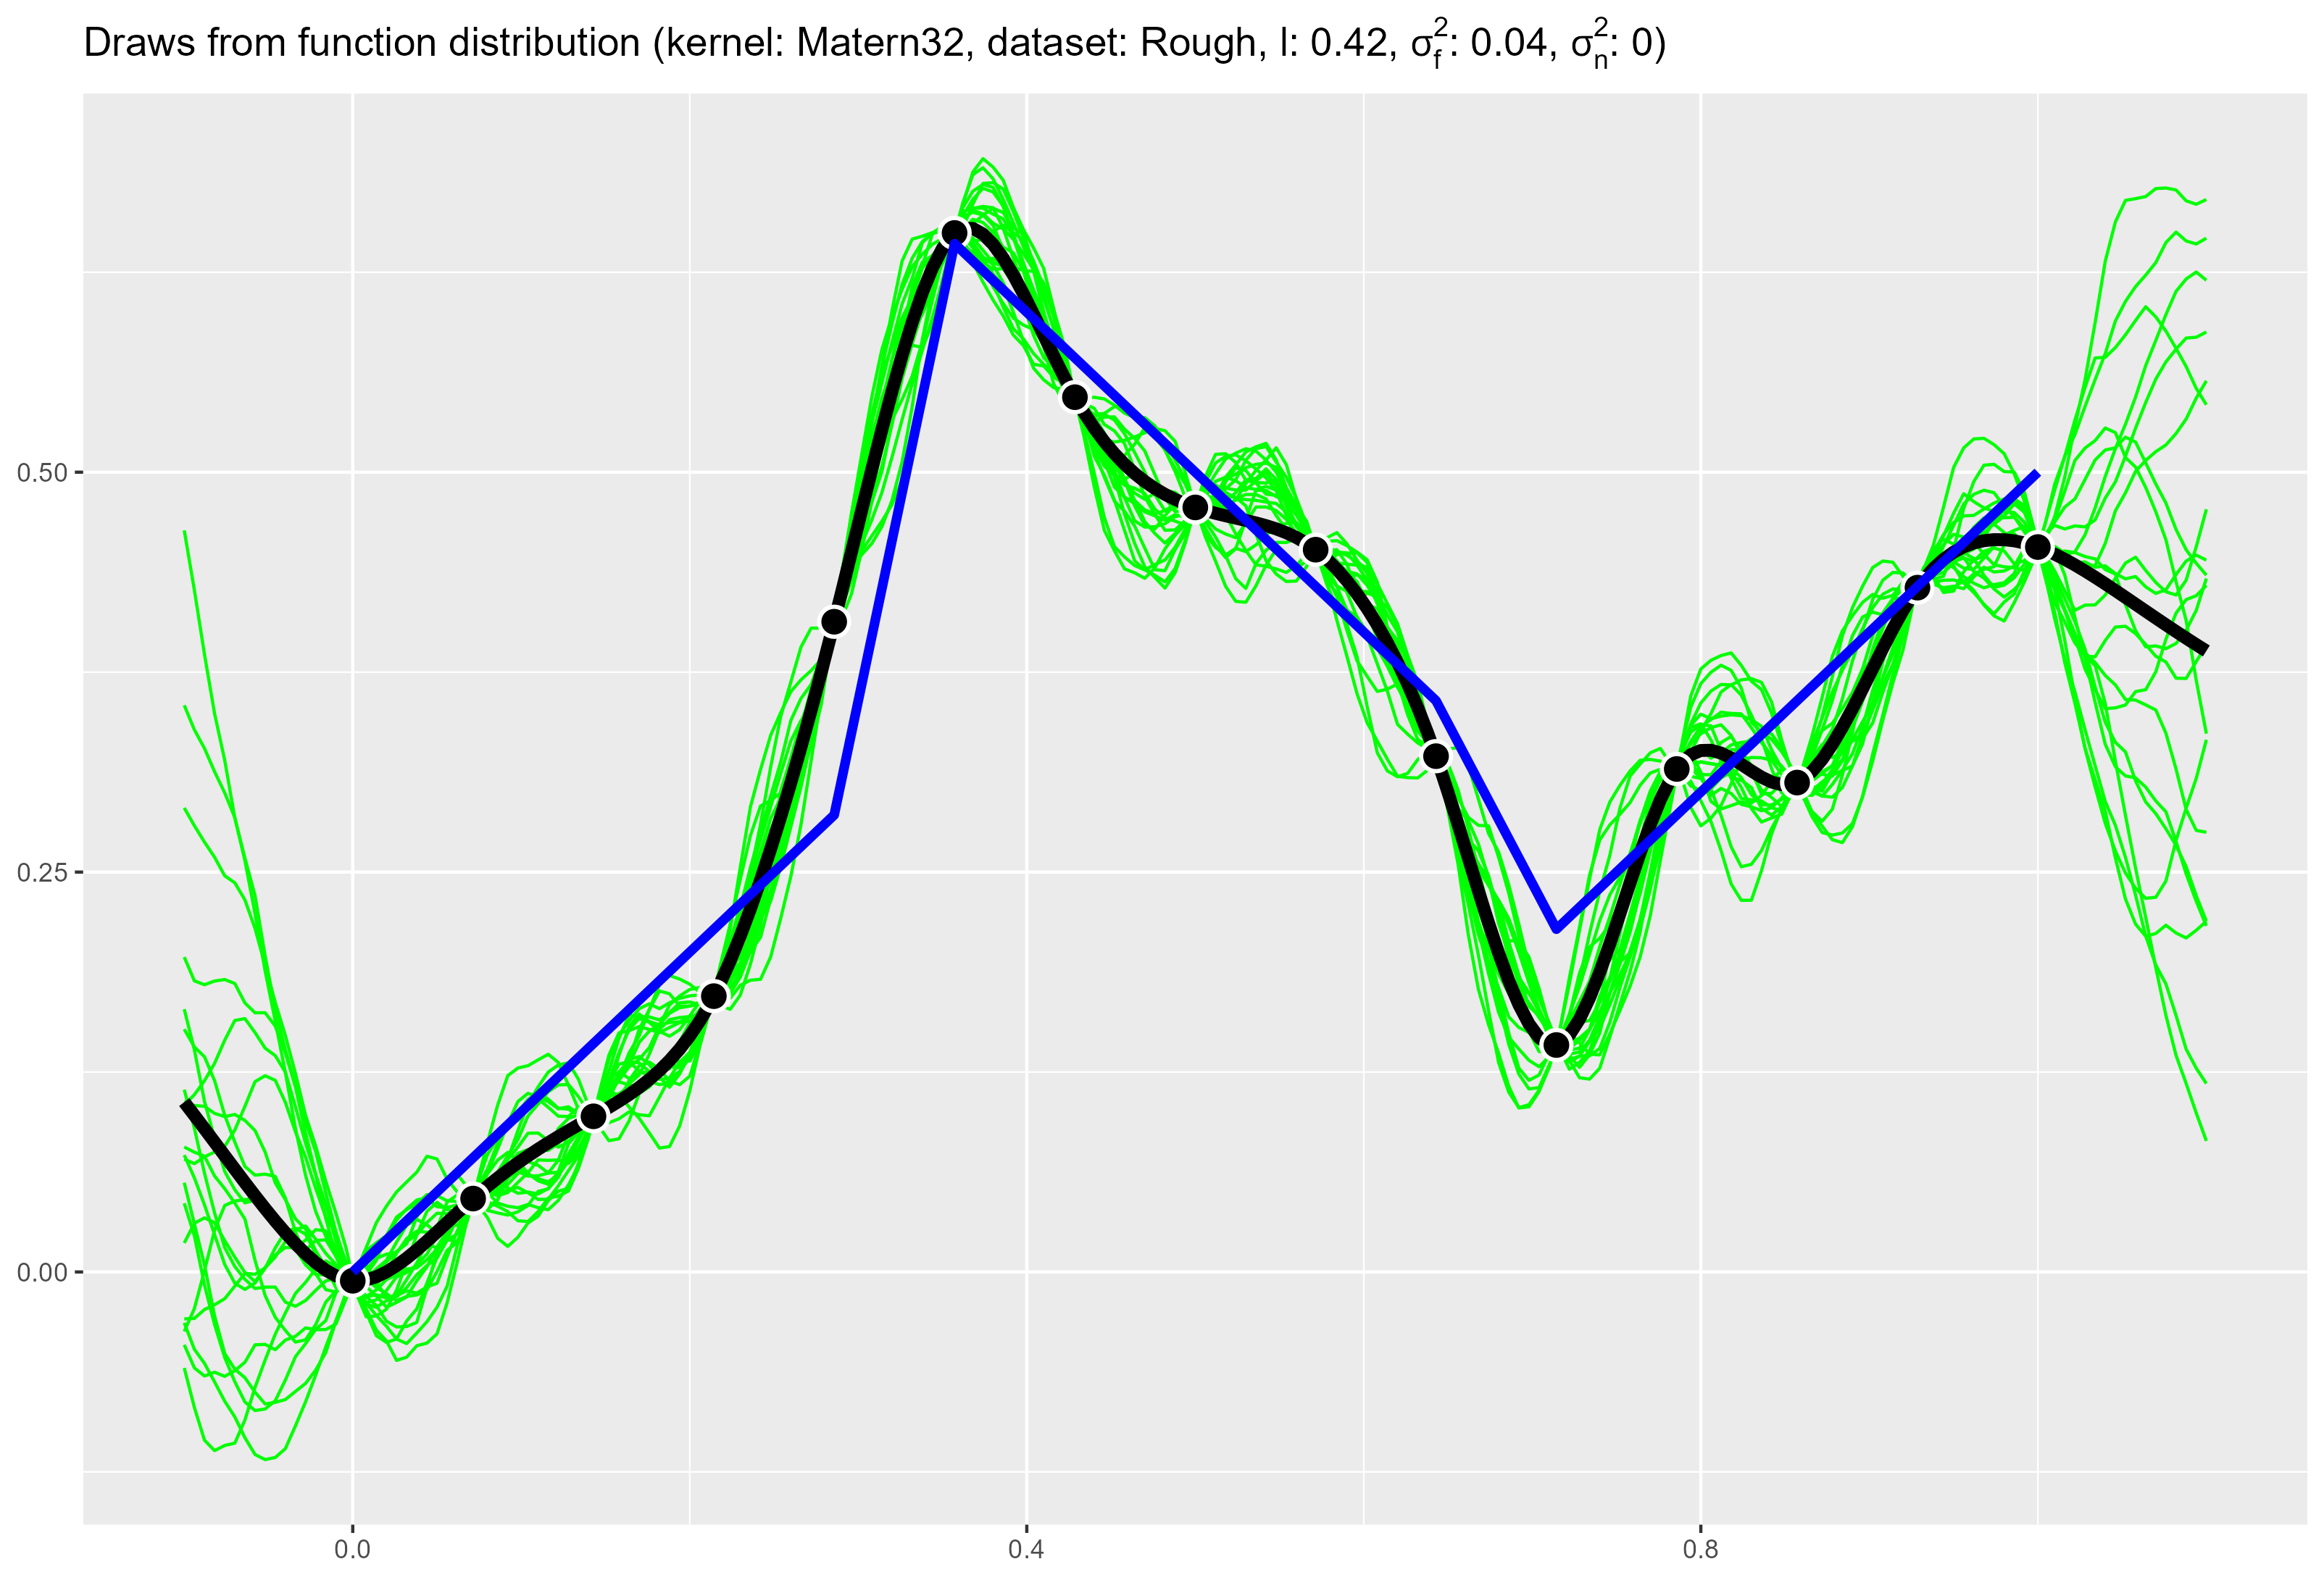
\includegraphics[height=0.5\textwidth]{covariance-functions/Matern32_Rough_draws.png}
    \caption{
        Plots of some sample functions drawn from a GP as before, trained on the rough dataset using Matern 3/2.
    }
\end{figure}
Although these function draws are much smoother than those produced by the exponential covariance function, they are still rough between points.

% Matern 3/2: Assumes one time differentiability. This is often too low of an assumption. \cite{gaupro}

\paragraph{Matern 5/2}
$\nu = 5/2$ produces the following covariance function:
\begin{equation*}
    k_{5/2}(X,X') = \left(1 + \frac{\sqrt{5}|X - X'|}{l} + \frac{5|X - X'|^2}{3l^2} \right) \exp \left(-\frac{\sqrt{5}|X - X'|}{l} \right)
\end{equation*}
5/2 is twice MS differentiable, producing functions that are slightly smoother than 3/2. 

This is the most commonly used stationary covariance function \cite{gaupro} because it represents a sweet-spot between the smoothness of SE and the roughness of exponential, and is able to adapt to a wide range of data-generating functions.

\begin{figure}[H]
    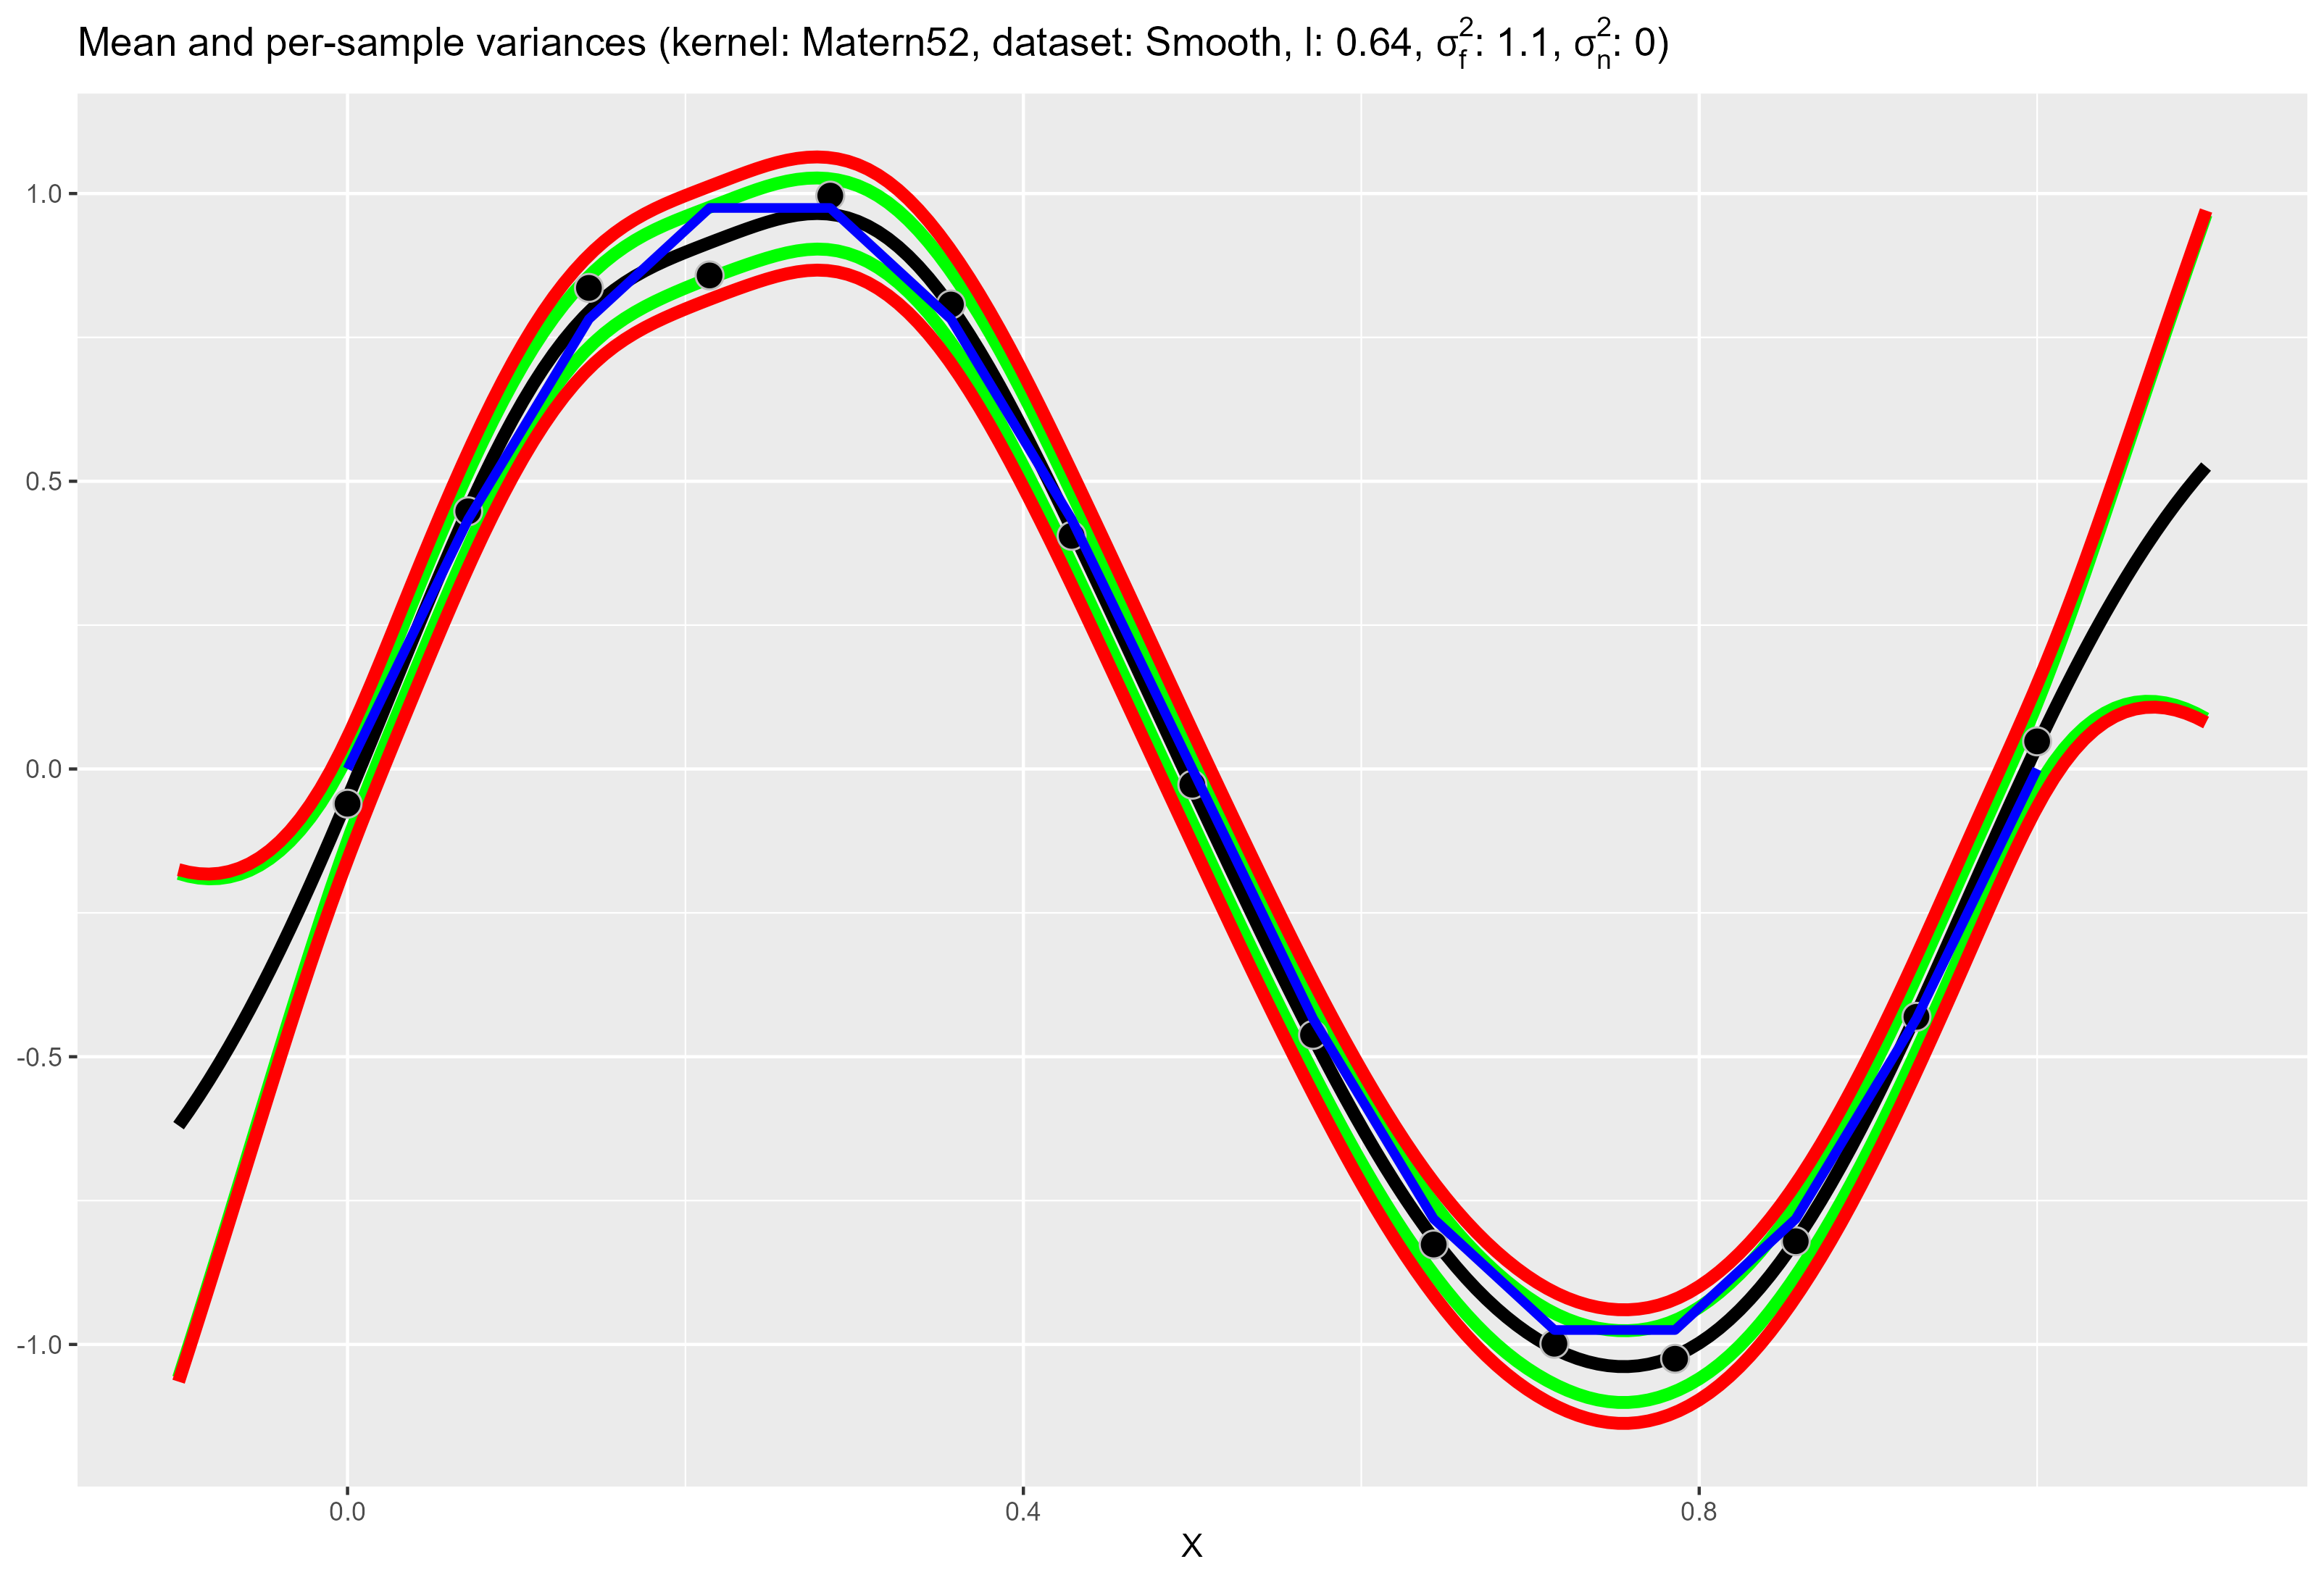
\includegraphics[height=0.5\textwidth]{covariance-functions/Matern52_Smooth_mean.png}
    \caption{
        Plot of the expected function draw and variances as before, using Matern 5/2 fitted to the smooth sin wave dataset. 
    }
\end{figure}
Here, Matern 5/2's expected function is smooth enough to resembles SE - a smooth function that did not pass through all training points. The variance of the noise-free function evaluations and the noisy observations are narrower than SE's, as the additional roughness allows the expected function draw to pass closer to the training points. For example, the previously examined point at $(0.21, 0.86)$ is now much closer to the expected function draw than under SE.

\begin{figure}[H]
    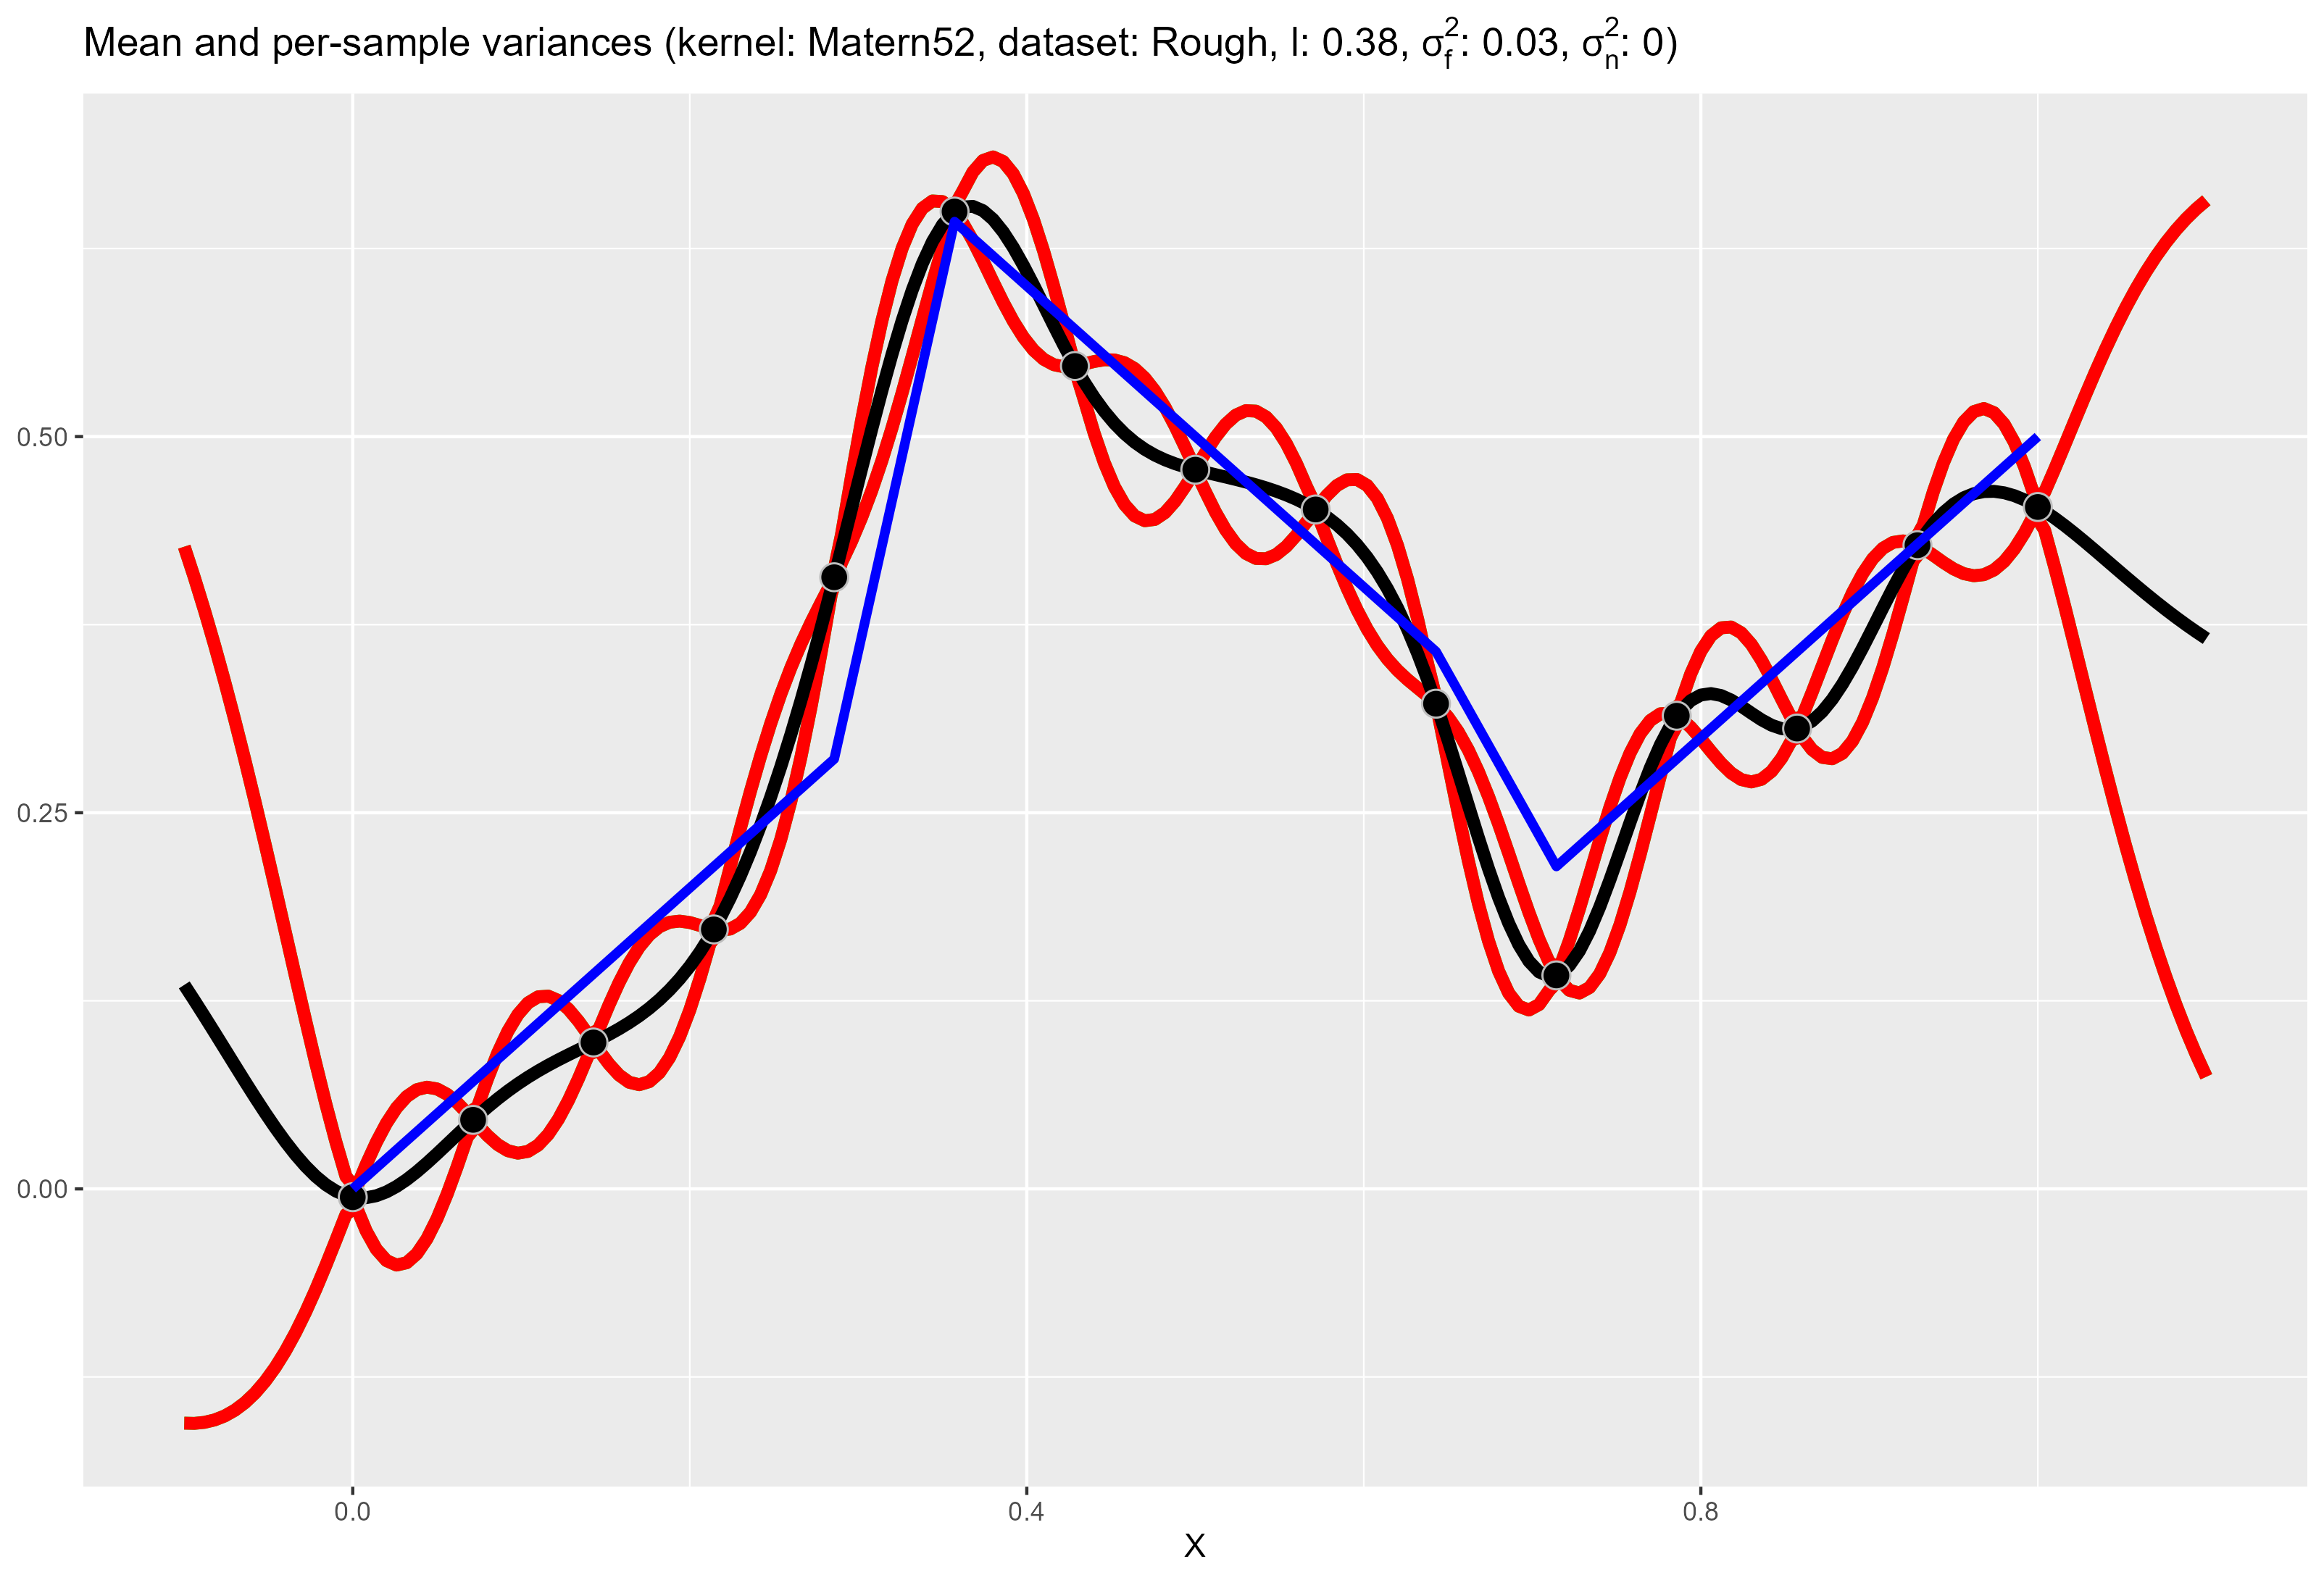
\includegraphics[height=0.5\textwidth]{covariance-functions/Matern52_Rough_mean.png}
    \caption{
        Plot of the expected function draw and variances as before, using Matern 5/2 fitted to the rougher dataset. \\ 
    }
\end{figure}
Matern 5/2 has adapted well to the rough dataset - the expected function draw is smoother than the expected function draw from Matern 3/2, but remains rough enough to pass through all training points. The variances are the narrowest of all the covariance functions because the smoothness constraint is severe enough to prevent exponential-style white noise, but the roughness is high enough to approach the training points closely. 

\begin{figure}[H]
    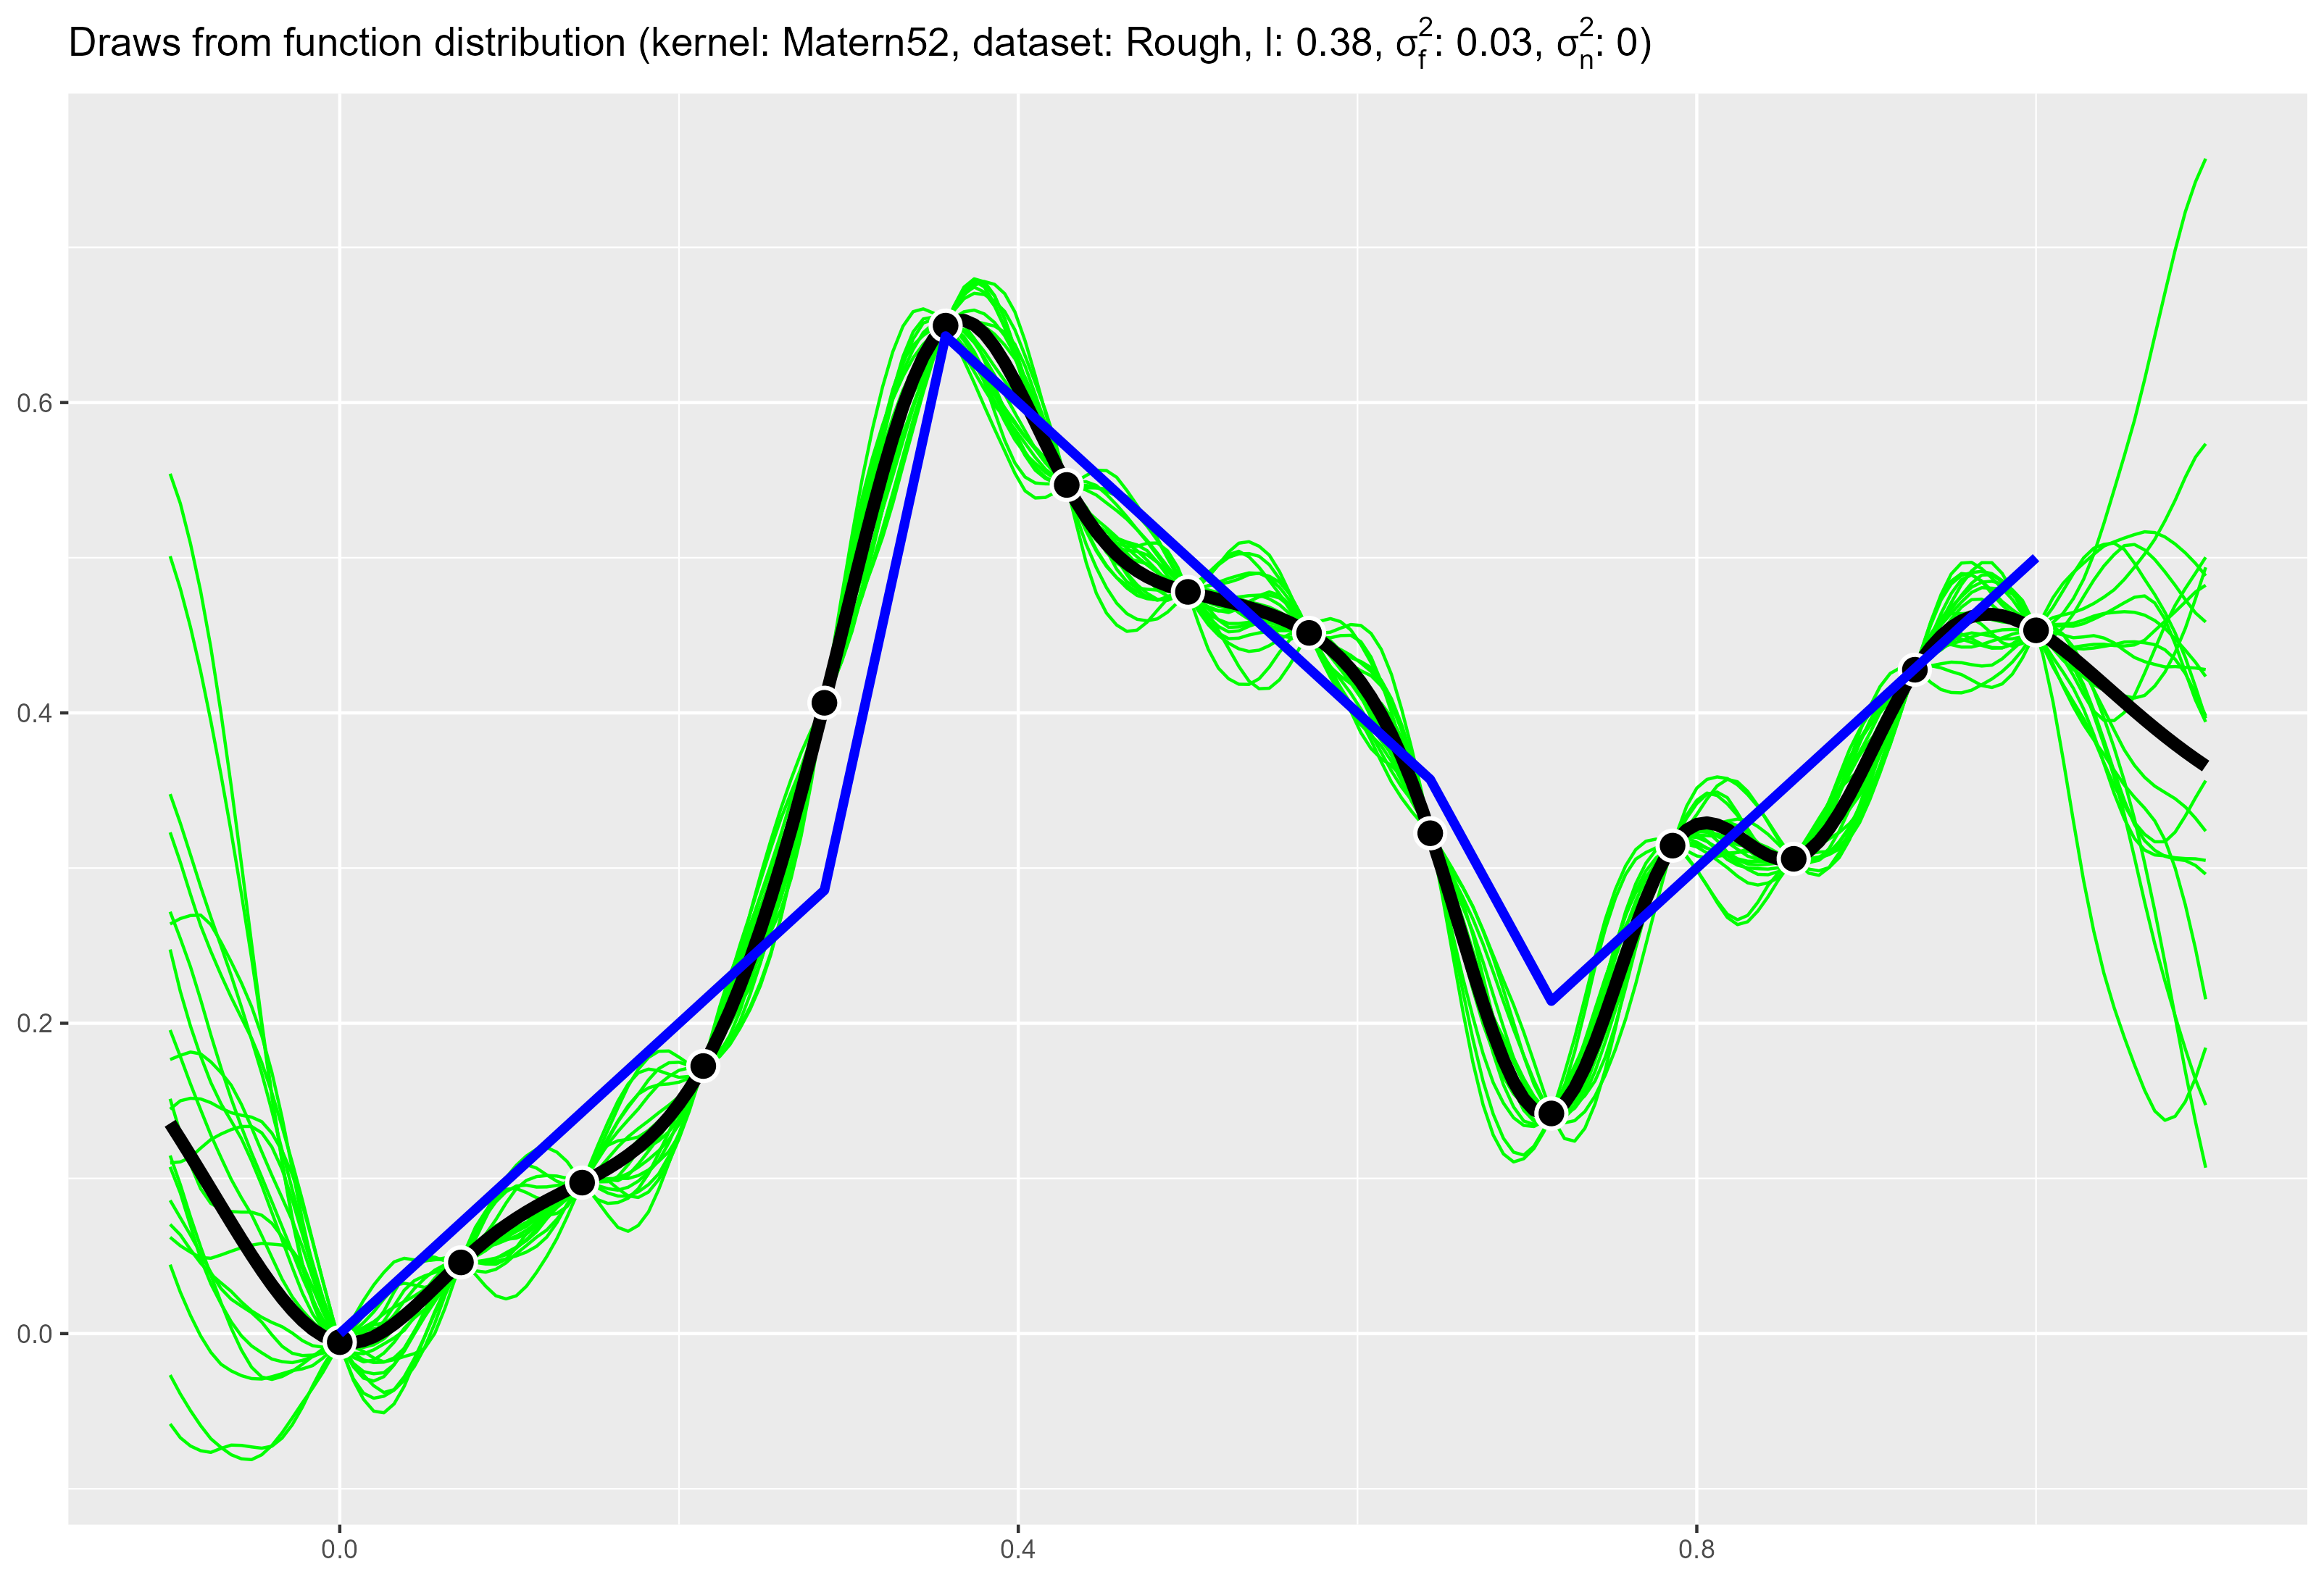
\includegraphics[height=0.5\textwidth]{covariance-functions/Matern52_Rough_draws.png}
    \caption{
        Plots of some sample functions drawn from a GP as before, trained on the rough dataset using Matern 5/2.
    }
\end{figure}
These function draws are much smoother than those drawn from Matern 3/2, particularly between data points, whilst still passing through all datapoints.

% Matern 5/2: Assumes two time differentiability. Generally the best. \cite{gaupro}




% \subsection{Non-stationary covariance functions \cite{gp-ml}}
% 
% \subsubsection{Sum and product}
% 
% \subsubsection{Neural network}
% 
% \subsubsection{Warping and periodicity}


% \subsection{Language-processing covariance functions \cite{gp-ml}}
% 
% \subsubsection{String}
% 
% \subsubsection{Fisher}
% 
% 
% \subsection{Factor-processing covariance functions \cite{gaupro}}
% 
% \subsubsection{Ordered factor}
% 
% \subsubsection{Factor}
% 
% \subsubsection{Gower factor}
% 
% \subsubsection{Indices-ignoring}


% \subsection{Deriving kernels \cite{deriving-kernels}}
% 
% \subsection{Learning best kernel from data \cite{choosing-kernels}}

% \subsection{Additive covariance kernels for high-dimensional learning \cite{additive-kernels}}
% 
% 
% \subsection{Hierarchical Bayesian covariance function for hierarchical modelling \cite{hierarchical-kernels}}
% 
% 
% \subsection{Free-form covariance matrix for multi-task learning \cite{freeform-kernels}}
% 
% 
% \subsection{Combining different kernels for multi-task learning \cite{multi-kernels}}



% \section{Extensions of the Gaussian Process}
% 
% 
% \subsection{Gaussian process regression networks \cite{gprn}}
% 
% 
% \subsection{Variational Gaussian process \cite{vgp}}
